% MSc dissertation example file, February 2022
%
% Leave one of the documentclass lines uncommented to match your degree.
% You may remove the logo option if it causes problems.
% Do not change any other options.
% \documentclass[logo,msc,adi]{infthesis}     % Adv Design Inf
% \documentclass[logo,msc,ai]{infthesis}      % AI
% \documentclass[logo,msc,cogsci]{infthesis}  % Cognitive Sci
% \documentclass[logo,msc,cs]{infthesis}      % Computer Sci
% \documentclass[logo,msc,cyber]{infthesis}   % Cyber Sec
% \documentclass[logo,msc,datasci]{infthesis} % Data Sci
% \documentclass[logo,msc,di]{infthesis}      % Design Inf
% \documentclass[logo,msc,dsti]{infthesis}    % Data Sci TI
% \documentclass[logo,msc,inf]{infthesis}     % Informatics
\documentclass[logo,msc]{infthesis}           % degree unspecified, do not change except to add your degree
%%%%%%%%%%%%%%%%%%%%%%%%
% Understand any problems and seek approval before assuming it's ok to remove ugcheck.
\usepackage{msccheck}

% Include any packages you need below, but don't include any that change the page
% layout or style of the dissertation. By including the ugcheck package above,
% you should catch most accident-al changes of page layout though.
%\documentclass{article}
\usepackage{mathtools}
\usepackage{microtype} % recommended, but you can remove if it causes problems
\usepackage{graphicx}
\usepackage{subfig}
\usepackage{algorithm}
\usepackage[lined,boxed,linesnumbered]{algorithm2e}
\usepackage{algpseudocode}


\begin{document}
\begin{preliminary}

\title{Machine Learning of Polyhedral Compilation}

\author{Prakshal Nandi}

\date{\today}

\abstract{

In most compute-intensive applications, a considerable amount is spent in loops. Compilers like clang offer many optimisations, such as tiling, fission, fusion, and unwinding, to increase the execution performance of these loops. One of the ways to optimise loop performance is through polyhedral compilation strategies, which apply to a specific class of loops. If the loops follow a specific structure, it is possible to change the execution order of the loop statements to make the program run faster. However, this requires domain-specific knowledge to design suitable heuristics, which is also difficult to generalise. \par
This study set out to examine the possibilities of using Reinforcement Learning algorithms to apply semantics-preserving transformations to optimise the schedule of the loop execution. As a background to this research, PolyGym \cite{P1} has already presented Polyhedral Compilation as an environment of Reinforcement Learning. We continue this investigation by implementing Q-learning agents to construct the number of valid schedules and then explore the schedule space to find a highly effective schedule using RL algorithms. We demonstrate that we can generalise the learning on PolyBench\cite{polybench} kernels and achieve a mean speedup of 2.11x compared to clang -O3 flag.
}

\maketitle

\newenvironment{ethics}
   {\begin{frontenv}{Research Ethics Approval}{\LARGE}}
   {\end{frontenv}\newpage}

\begin{ethics}
This research does not involve any human participants or personal data. All data are collected based on simulation experiments on benchmark suites; hence no ethical concerns are associated with the project.

\standarddeclaration
\end{ethics}


\begin{acknowledgements}
Any acknowledgements go here.
\end{acknowledgements}


\tableofcontents
\end{preliminary}


\chapter{Introduction}

\section{Motivation}

Recently, there have been many advancements in machine learning for compiler optimization. One class of optimizations among these is finding the performant schedule for the nested loops following specific properties. However, this involves many complex decisions and presents a high entry barrier requiring domain knowledge. The idea behind using machine learning for this purpose is to reduce human intervention, which also allows building modular compliers facilitating the application of transformations. Reinforcement Learning is currently seen as a promising approach where the agent can iteratively build a high-performing code by taking actions and learning from the observations.\cite{8357388}\cite{9232934}. PolyGym has leveraged the Polyhedral model and presented an environment for Reinforcement Learning to learn the heuristics for composing performant schedules. It proposes a generic MDP to apply transformations but does not define any agent. \break
As a first point, we develop a Q-Learning RL agent from the literature\footnote{https://github.com/prakshalnandi/polygym}. We define the state features using the polyhedral model, which will provide observations for RL algorithms. We compare the performance of the schedule generated using this approach with simple heuristics and also explore different variations of the configurations. This will be a stepping stone in an emerging and promising field of machine learning for compilers and provide a basis to experiment further to implement more advanced combinations of machine learning algorithms.



\section{Objectives}

The importance and originality of this study are that it explores how Reinforcement Learning can help improve Polyhedral Compilation.  We hypothesise that Reinforcement Learning algorithms can be generalised to learn Polyhedral Compilation.

This dissertation seeks to find the answers to the following objective questions:
\begin{itemize}

    \item Can we extract the representable and learnable features of the kernels, leveraging the polyhedral model, which Reinforcement Learning can utilise? 
    \item Can we generalise the Q-Learning agent to learn to formulate the profiting schedules irrespective of the target kernel?
    \item Can we design a reward function that can be trickled down to all the state action pairs in the transactions?

\end{itemize}

\section{Structure}

The overall structure of the thesis takes the form of five chapters. Following the current chapter, chapter two begins by laying out the theoretical concepts such as Polyhedral Compilation and Reinforcement Learning, and looks at the recent literature history of this subject. The third chapter is related to the methodology used for this study. The next chapter gives an overview of the evaluation and looks at how experiments were performed. It will then go on to present the research findings and results. Chapter Six concludes the study and discusses unresolved issues and future work.

\chapter{Background}

\section{Polyhedral Compilation Model}

 The polyhedral model is the basis for applying affine loop transformation on the fine-grained loop representation in the form of polytopes. A simple two-dimensional nested loop is shown in Figure \ref{fig:Polly_Loop}. There are different ways in which this loop can be optimized, including changing the order execution, cache locality, data location, vector instructions, parallel threads and tasks. The execution of this loop next can be executed in the order shown in \ref{fig:Loop_Schedule}. The individual loop operation we perform can be written down as a point in a two-dimensional vector space, Figure \ref{fig:Loop_Str}. In general, there are more than two dimensions. We could generalize this representation in the form of polytopes to represent this set of points more concisely. This polyhedron can be described as a set of linear constraints we must adhere to while applying the transformations, Figure \ref{fig:Loop_Ineq}. Thus, an n-dimensional mathematical model like polytope can represent the iteration space of a nested loop \cite{P3}. This iteration space of the kernel can be described as in Equation \ref{eq:I_space}. The time when these iterations are performed, i.e. the schedule, can be described as in Equation \ref{eq:S_space}. If we want to change the performance of the program runs, we only need to change this execution schedule. Notably, the loop interchange can be implemented here by just changing the schedule from \textit{(i,j)} to \textit{(j,i)}. The polyhedral Model is widely applicable as affine loops are quite common in applications involving many computations \cite{poly_applicable}.

\begin{equation}
I_s = \{S(i,j) \hspace{2} | \hspace{2} 1 <= i <= n \hspace{2}, \hspace{2} 1 <= j <= i\}
\label{eq:I_space}
\end{equation}

\begin{equation}
\theta_s = \{S(i,j) \hspace{2} \Rightarrow (i,j) \}
\label{eq:S_space}
\end{equation}

The optimization through Polyhedral Compilation is achieved in three stages: moving from code to polyhedron model, applying program transformations within the model, and finally regenerating the code from the model. This model gives the framework to transform the loops, where the array references and loop bounds are affine functions of loop iterators and parameters. The polyhedral model is broadly applicable due to the high presence of affine loops in compute-bound applications\cite{poly_applicable}. In the kernel example shown in Figure 1, geometric interpretations such as two-dimensional polygons can be used to visualize dependencies between statements. Using the information provided by these dependencies, the execution time of each statement can be changed without affecting the correctness of the output. 

\begin{figure}[!tb]
  \centering
  \subfloat[Polly Loop.]{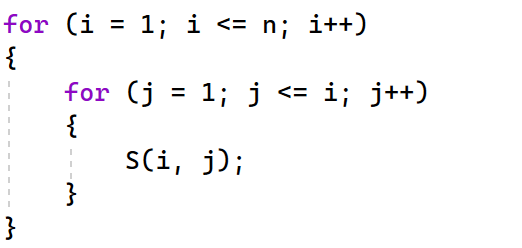
\includegraphics[width=0.5\textwidth]{Images/polly_loop.png}\label{fig:Polly_Loop}}
  \hfill
  \subfloat[Structure of loop.]{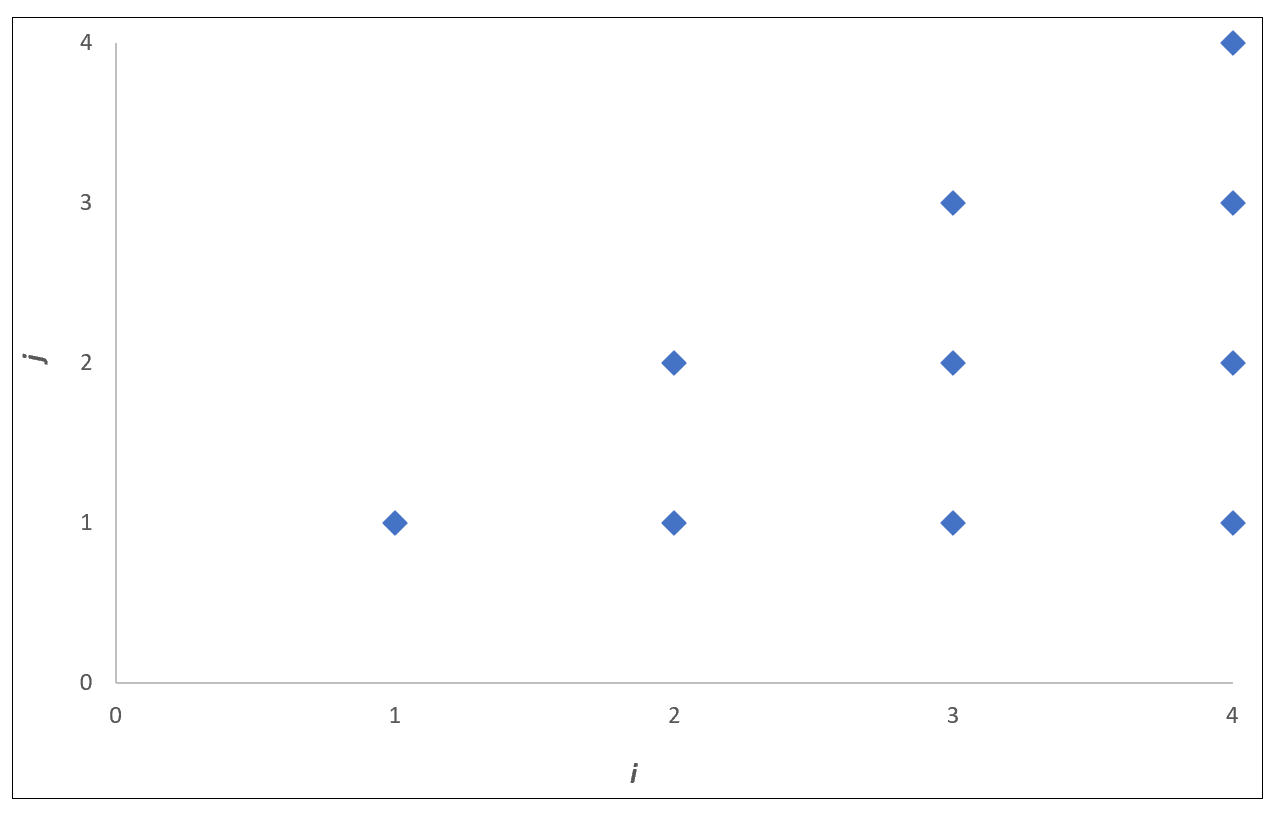
\includegraphics[width=0.5\textwidth]{Images/loop_structure.png}\label{fig:Loop_Str}}

  \centering
  \subfloat[Schedule of Loop Execution for n=4]{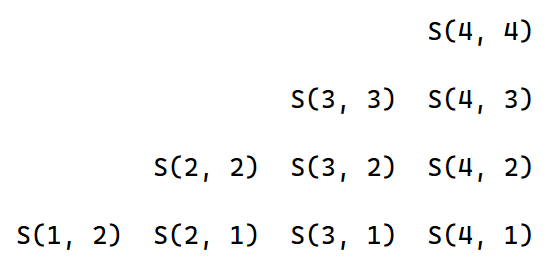
\includegraphics[width=0.5\textwidth]{Images/loop_schedule.png}\label{fig:Loop_Schedule}}
  \hfill
  \subfloat[Loop Inequalities]{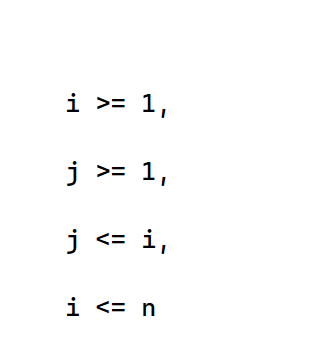
\includegraphics[width=0.45\textwidth]{Images/loop_inequalities.png}\label{fig:Loop_Ineq}}
  
  \caption{Polyhedral Representation of Loop Execution}
\end{figure}



\section{PolyGym}

The geometric properties of the dependencies between two statements during loop iteration execution can be defined as space of constraints. Exploration of this space offers an opportunity to apply semantics-preserving transformations to improve the performance of the loop. This exploration mainly has two methods: problem-specific heuristics \cite{isl} \cite{Bondhugula07pluto:a} or iterative meta-heuristics\cite{it_Single}\cite{it_multi}. The latter approach yields better results but is time-consuming and challenging in practical applications. Reinforcement Learning presents a middle way among these approaches. However, all the challenges applicable to polyhedral compilation still exist in the Reinforcement Learning problem. For example, if the actions in an RL environment are related to direct transformations, these transformations may not apply to all the loops in practice. Moreover, it is not straightforward to generalise the problem and the learning of the agent.

Polygym presents an RL environment for Polyhedral Optimization\cite{PolyOpt}, where the transformations are applied using actions selected through a loop-agnostic Markov Decision Process, adhering to OpenAI Gym interface \cite{Gym}. First, it constructs a search space of the transformed schedules by applying Farkas' lemma \cite{schrijver1998theory} to generate a set of linear inequalities from the affine functions representing the schedule. The next step navigates this search space to find the highly profitable schedule using the generators obtained by Chernikova's algorithm. The original implementation of Polygym did not intend to offer any optimization strategy, though it used a random heuristic to evaluate the environment space. Even by using this simple heuristic on the space defined by PolyGym, it was possible to find profitable schedules with an overall 3.39x speedup over those found using o3-clang12 and 1.34x speedup over \textit{isl-polly12}. However, Polygym neither uses any agent nor implements any learning behaviour. Moreover, this heuristics is specific to the particular loop under testing and not generalised. This thesis demonstrates the results of using agent-based RL methods to generalise the learning and evaluate its performance building up on Polygym implementation.

\section{Deep Reinforcement Learning}

The problem of reinforcement learning can become challenging if the number of states possible in the environment is too vast. Deep Learning addresses this challenge by approximating the Q-values of the state and action pairs using model parameters called weights. The framework of a neural network consists of an input layer, an output layer and one or more intermediate layers. The neurons in the layer have weights associated with them, which we are trying to optimize. The output generated by the network is compared with the target, and loss will be calculated. Different loss functions are available for comparisons, such as mean square error, cross-entropy loss or maximum likelihood loss. They all represent how far the model's output is compared to the desired result. Once we know the loss value, the gradients can be calculated considering the effect of each parameter on the output. Using an optimizer, such as SGD, Adam, or RMSprop, we can change the weight values to reduce the loss using the calculated gradients. We are moving towards the desired result by doing this in an iterative manner. Performing all these steps manually could help understand how deep learning works, but it could quickly get complicated in practical applications. Luckily, we have libraries such as PyTorch, which can calculate the gradients and perform backpropagation (explain backpropagation) to develop new network parameters. A classic example of what can be done when Deep Learning and Reinforcement Learning come together is AlphaGo \cite{AlphaGo}, developed by DeepMind, which successfully beat the world champion of the game of Go at that time. Prior to that, DeepMind had been using Deep Reinforcement Learning to solve the Atari games and achieve human-level performance\cite {DeepMind}.

\section{PyTorch}

PyTorch implements a dynamic graph approach for gradient calculation, where the library keeps track of the operations performed on the data and unrolls this operation sequence when we need to calculate the associated gradients. The basic building block of DL is the \textit{tensor}, representing a multi-dimensional array, which is also implemented by this toolkit. PyTorch has methods to create tensors, convert numpy arrays to tensors, and generate tensors with specific data, such as \textit{torch.ones()}. It can also apply different tensor operations to concatenate, resize and transpose them. The library also allows for offloading the tensor calculations to GPU by specific the \textit{}device property associated with it. A tensor may or may not have gradient construction available, and this behaviour can be configured and retrieved using properties such as \textit{requires\_grad} and \textit{grad}. By using \textit{backward} operation, we can ask PyTorch to calculate the gradients of all the variables in the network. By leveraging \textit{nn.Module} of PyTorch, we can define the network architecture, design dropouts, reinitiate the gradients and apply transformations such as \textit{Softmax}.

\section{Clang/LLVM/Polly}

LLVM is a set of optimizer libraries built around an intermediate representation of the code known as LLVM-IR. Like many other analyzing and optimizing tools, it uses the Clang frontend, a \textit{C} language family compiler, as a library.
Polly applies polyhedral transformations on top of this intermediate representation\cite{grosser2011polly}. It first identifies relevant regions of the code suitable for transformations, called Static Control Parts(\textit{SCoP})\cite{grosser2011polly}. It then transforms these regions into a polyhedral representation based on integer sets and maps. In this representation, it applies optimizations, for example, related to data locality and parallelism, finally converting it back into the optimized version of the executable code. As Polly analyses the low-level IR instead of the programming language itself, it is not dependent on any language or platform.

A \textit{SCoP}, generally consisting of loops and conditions, contains part of the program for which control flow and memory access can be determined at the compile time. For a loop to be identified as \textit{SCoP}, the scalar expression for the iteration count should be able to be represented as an affine function. Similarly, the memory accesses for loading and storing should also be possible to be translated into an affine expression. Polly allows the export of this polyhedral representation into a \textit{JSON} based format called \textit{jSCoP},
allowing us to apply external optimization, which can be imported back using the same \textit{jSCoP} format.

 Figure \ref{fig:Original_Loop} showcases an example of a \textit{C} loop doing matrix multiplication. Using \textit{clang}, we can identify the \textit{SCoP} parts of the code and convert them into LLVM representation as displayed in Figure \ref{fig:Poly_Rep}. The representation consists of statements as basic building blocks. Apart from its name, a \textit{statement} consists of \textit{Domain}, \textit{Schedule} and \textit{Access}. The \textit{Domain} represents a set of different loop iterations executing the statement as a named integer set. The \textit{schedule} is an integer map which assigns a point to each iteration in a multi-dimensional space following lexicographical order. Changing the schedule will change the order in which the kernel is executed. \textit{Access} is a pair of kind and relation. The kind can be either \textit{read}, \textit{write} or may \textit{write}. The access relation maps the Domain with the memory space, which generally can be represented by an affine function. Figure \ref{fig:Dependencies} explains the dependencies information extracted from the above representation, which can exist between two statements or two iterations of the same statement. When the transformations have been applied, AST can be generated from the LLVM representation as shown in Figure \ref{fig:AST} and the program can be executed\cite{10.1145/2743016}.

 \section{Q-learning}

 The value of a state can be defined as the expectation of the maximum reward which can be gained from that state, considering all the actions that can be taken in that state. To select the optimal actions, we will need to determine the values of each action and choose the one with the best possible result. In a way, the value of a state corresponds to the value of the action we can take from this state, giving us the maximum possible outcome.

 The state-action value can be represented as mentioned in Equation \ref{eq:SAQV} (sn - change this),

\begin{equation}
Q(s,a) = r(s,a) + {\gamma} max_{a'\in A} Q(s',a')
\label{eq:SAQV}
\end{equation}
 
 A Q-Network can be trained by minimising the loss function at each iteration as shown in Equation \ref{eq:DQN} (sn - change this),

\begin{equation} L_{i}(\theta _{i}) = E_{s,a\sim\rho(\cdot)}[(y_{i} - Q(s,a;\theta _{i}))^2]
\label{eq:DQN}
\end{equation}

where \(y_{i} = E_{s'\sim\epsilon}[r+\gamma\max\limits_{{a'}}Q(s', a'; \theta_{i-1})|s, a]]\) is the target for iteration i. \(\rho(s,a)\) is the probability distribution over states s and actions a. \(\gamma\) is the discount factor, r is the reward, and \(Q(s,a;\theta)\) is the function approximator to estimate the action-value function \cite{DBLP:journals/corr/MnihKSGAWR13}.

\section{Value Function Approximation}

Any form of tabular learning like Q-Learning requires we visit each state multiple times and apply all the available actions to estimate the correct Q-Values. However, this is impractical in most real-world scenarios, especially those involving a vast state space. Also, it takes up a lot of memory to save and update the Q-table containing many states and actions. One workaround is to approximate the Q-Functions using machine learning based on the visited states\cite{580874}. This will allow us to approximate Q-Value for a state-action pair \textit{(s,a)} even if action \textit{a} was never applied in the state \textit{s}. It will also help us to avoid maintaining a large Q table. Linear Function Approximation \cite{P2} is an excellent alternative to Deep Q-Learning here, as it is not as data-hungry as Deep Leaning and requires comparatively less computation.

\begin{equation}
Q(s,a) = f_1(s) * w_1^a + f_2(s) * w_2^a + ... + f_n(s) * w_n^a 
\label{eq:Q_Approx}
\end{equation}

\begin{equation}
w_i^a = w_i^a  + {\alpha} * {\delta} * f_i(S),
\label{eq:W_Approx}
\end{equation}

\begin{equation}
{\delta} = r + {\gamma} * max_{a'} Q(s',a') - Q(s,a)
\label{eq:delta}
\end{equation}

\section{Literature Review}

In the domain of compiler optimization, the space of possible transformations
, including their configurations and orderings are vast. Among these, which optimization to choose depend on the nature of the program itself and the hardware it is running on. Moreover, if the combinations of the optimization selected are not correct for the problem, it can actually degrade the performance.  As the compiler optimizations continue growing, the problem of selecting the effective combination of the optimizaantions is becoming more and more challenging.  With the growing complexities of the systems, software and security, the rate of improvement in the compilers has to keep up to help find answers to the open research problems \cite{compilerresearch}. There is a huge potential for the machine learning algorithm to explore this space, and it has been a topic of interest among researchers for a few decades. However, its success in the industrial compilers in the production environment has not been massive until now. In recent years though, there has been an increasing amount of literature on the subject of Machine Learning for Compiler Optimizations, which provides an excellent background to our research topic.

\cite{inproceedingsml} carried out one of the earliest attempts in this direction to use Machine Learning in branch prediction by giving the input of the branch history and making a prediction. Compy-Learn\cite{9232946} presented a toolbox to explore various representations and models of the code and choose the best one based on the task of the program. \cite{8357388} conducted a systematic review of the research directions undertaken in this field, discussing the importance of feature engineering and model generation and deployment. A significant analysis and discussion on the subject were also presented by Leather \textit{et al.}\cite{9232934}. Deep Learning reduces the dependence on the most accurate representation; rather, the agent will try to find the suitable features given that we provide enough data. This was demonstrated by Cummins \textit{et al.}\cite{inproceedingsdl} using neural networks to learn the code representation to find the best optimizations without using manually created code features.

Reinforcement Learning is seen as one of the most promising approaches for finding the correct strategy for applying optimizations\cite{9232934}. \cite{10.1007} showcased Markow Decision Process based learning(2014) to map the parallelism in the program with computing resources. They were able to adapt to varying resources and programs to predict the best thread mapping and obtained an average speedup of 2.14x over the default OpenMP policy. How to use Reinforcement Learning and Deep Learning in a combined way is no longer an open question, although it is evolving rapidly and a number of studies have begun to examine this method. In 2020, Neurovectorizer \cite{NeuroVectorizer} employed deep RL approach in LLVM compiler to take the code as input and implement vectorization. In the same vein,  Mammadli \textit{et al.} 
utilised deep reinforcement learning to address the long enduring problem of phase ordering. MLGO \cite{10.48550} used Policy Gradients and Evolutionary Strategies to reduce the size of the code with the help of function inlining. The nature of the optimization was different in this case as the focus was not to improve the heuristics to improve the execution speed.  Along the same lines pf PolyGym, CompilerGym \cite{CompilerGym} builds on top of OpenAI Gym interface and establishes an RL based environment for researchers to interact with compilers.

The basis of polyhedral conceptualisation was provided around three decades ago by Feautrier by converting the scheduling problem into a parametric linear program, first for one-dimensional time\cite{single} and then for the multidimensional time by using lexicographic ordering for schedules\cite{multi}. The actual application of polyhedral compilation was presented by Pouchet \textit{et al.} (2007) by construction and exhaustive exploration of single\cite{it_Single} and multi-dimensions\cite{it_multi} search space. Since then, researchers have built iterative methods on top of this. Ganser \textit{et al.} demonstrated how iterative optimization can be used for problems related to tiling and parallelization in compilers\cite{10.1145/3109482}. A year later, they proposed leveraging genetic algorithms to reduce the algorithm benchmarking time, but also losing the speedups by 15\% due to that. This methods of iterative optimization are time consuming, but not dependent on the program they are trying to optimize or the system resources. An alternative to this method are model based heuristics which are more direct but requires domain knowlege and are specific to the problem and system architecture\cite{Bondhugula07pluto:a} \cite{isl}. They are less time consuming compared to iterative meta-heuristics but do not meet the level of their performance. Reinforcement Learning can provide a middle way between the two approaches, reducing the time compared to iterative methods, but outperforming model based methods. 

\chapter{Methodology}

\section{Methods}

Figure \ref{fig:PolyGymRL} demonstrates a general workflow of PolyGymRL implementation. As an input, a program containing the kernel is provided to the stack of PolyGymRL, which generates a SCoP file. Two separate agents generate a new schedule using this representation and the new program is executed to calculate the speedup. The feedback on the performance of the new schedule is supplied to the agents to facilitate the learning. A detailed description of the software stack, construction and exploration phase is given in upcoming sections. One of the most critical aspects of this project is the training of the agents as described in Algorithm \ref{alg:agent_training}. Firstly, the environment and the agents for the construction and exploration are initialized. During the agent initialization, we provide values such as $\alpha$, $\gamma$, $\epsilon$ and the number of weights. There will be a few additional parameters depending on which form of Q-learning we are using. For example, we need to provide the number of weights if the Q-values are approximated. For a DQN agent, parameters like target update frequency and size of the network need to be provided. Once the initialization is completed, the agents are trained in two parts by running each kernel selected for training for the iterations defined by variable \textit{FLAGS.stop\_at} at the start.

\begin{figure}[htbp]
  \centering
  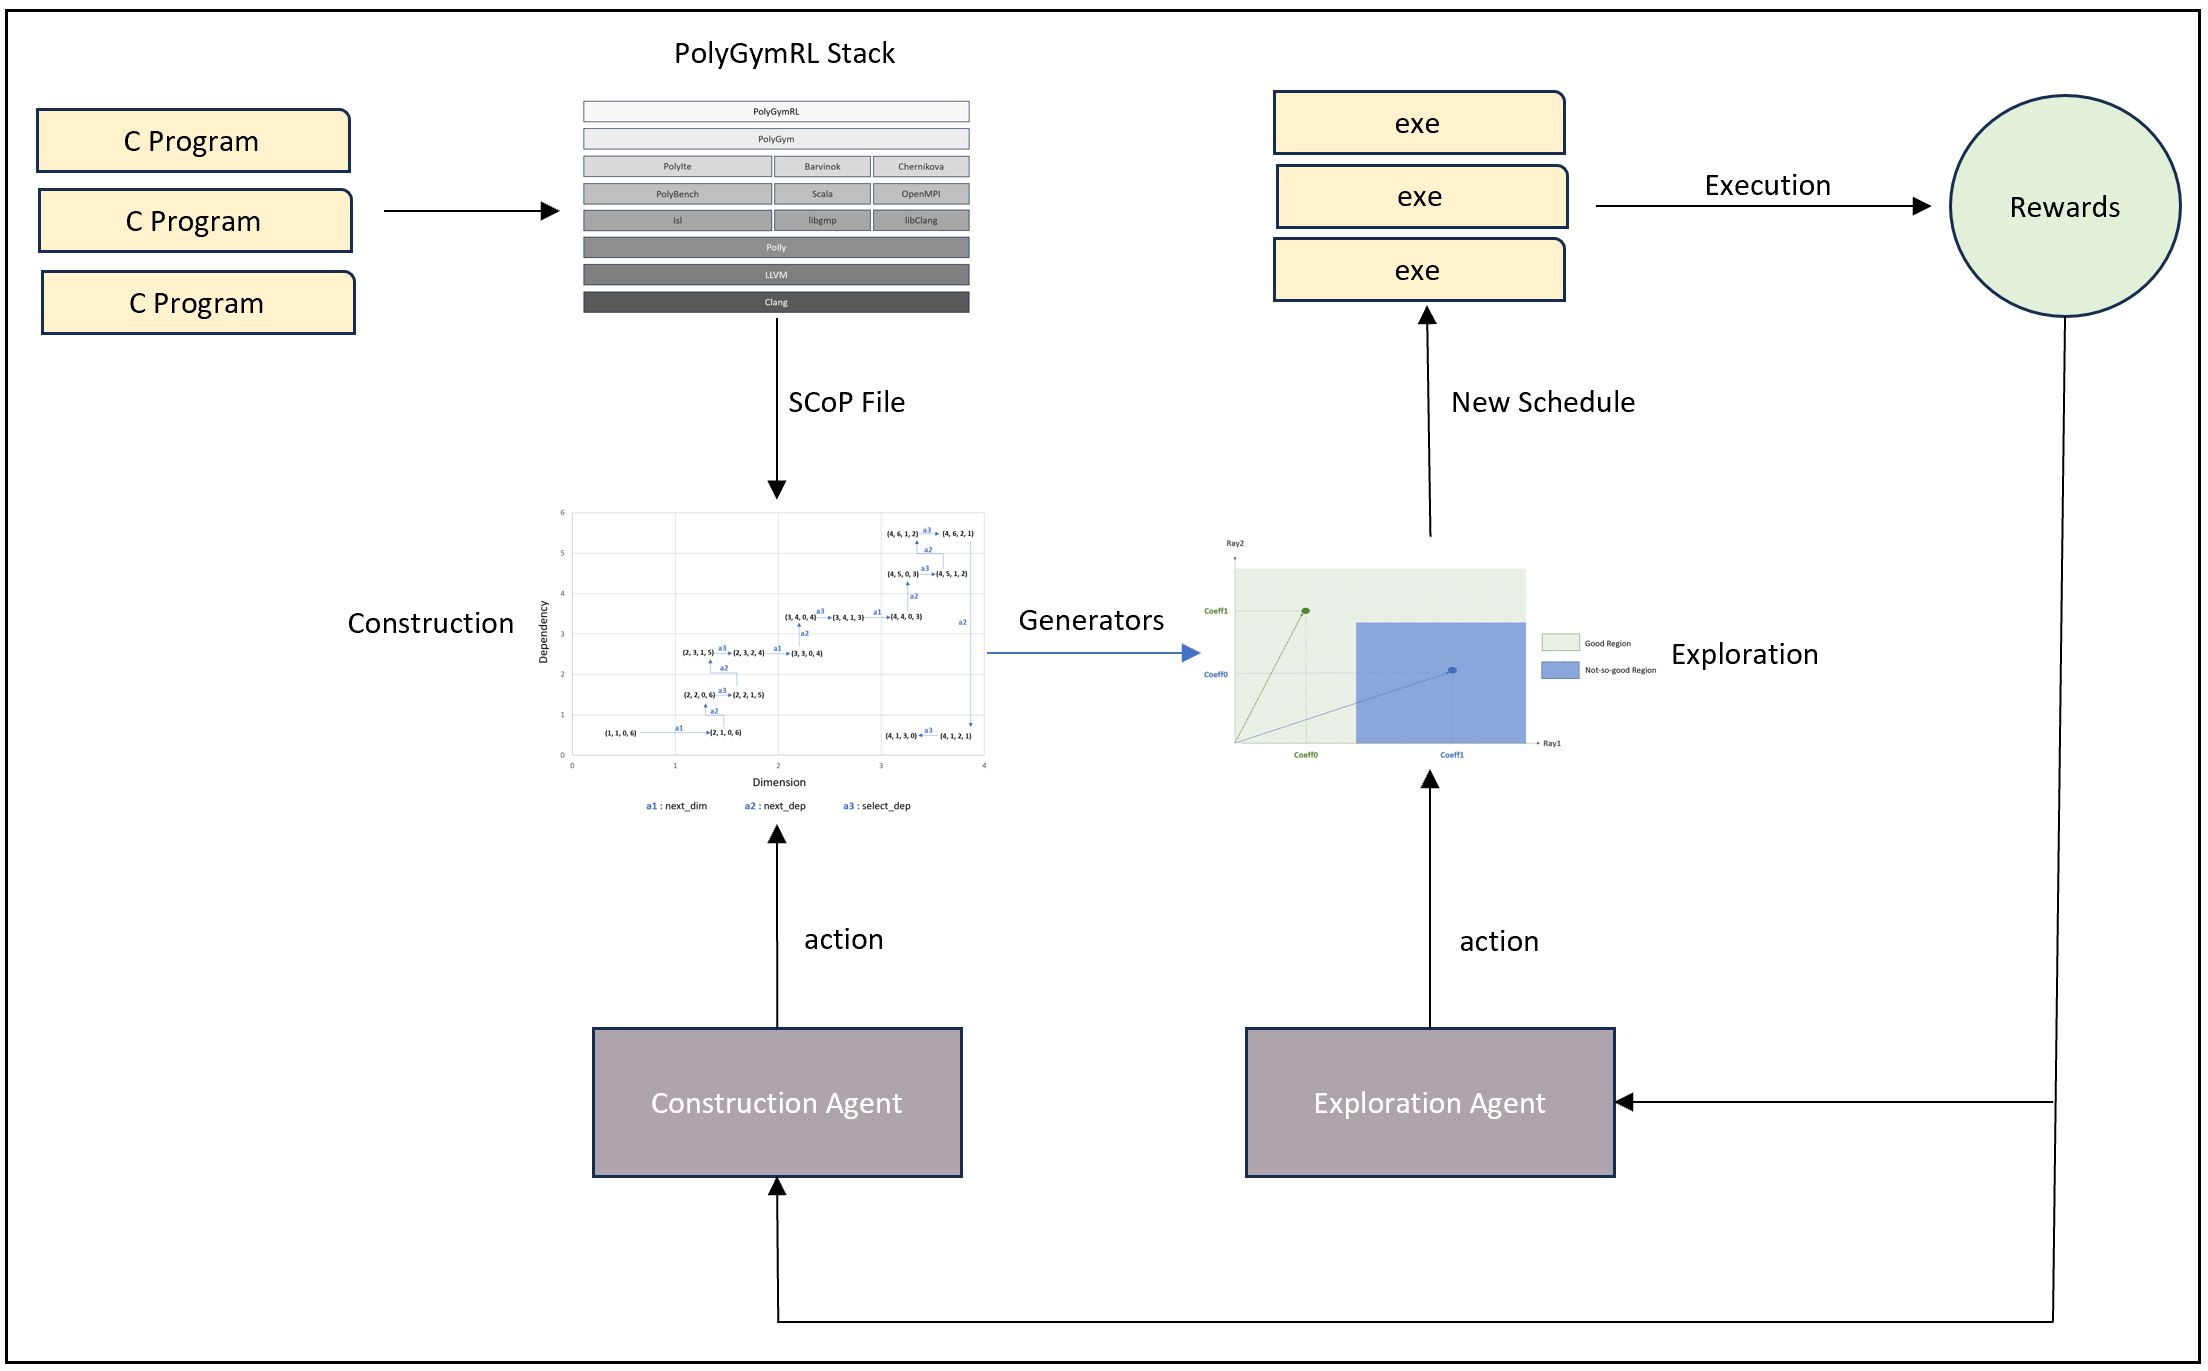
\includegraphics[width=0.9\textwidth]{Images/PolyGymRL.png}    
  \caption{PolyGymRL Workflow}
  \label{fig:PolyGymRL}
\end{figure}

In the first part, as described in Algorithm \ref{alg:generate_bench}, we generate a schedule and benchmark it, recording the states, actions, and rewards encountered during the process. Once the schedule is formulated and executed, we update the weights associated with the actions for different features as shown in Algorithm \ref{alg:weights_update}. If we work with a tabular Q-Learning algorithm, we update the Q-table associated with the state-action pairs instead of the weights. Once the training is over, we test the agent on a new kernel for the same number of iterations defined by \textit{FLAGS.stop\_at}, generating a schedule by choosing the actions decided by the trained agents. We take the geometric mean \cite{10.1145/5666.5673} of the speedup achieved during the evaluation.

\begin{algorithm}[H]
\caption{RL Agent Training and Evaluation}\label{alg:agent_training}
\SetKwData{Left}{left}\SetKwData{This}{this}\SetKwData{Up}{up}
\SetKwFunction{Union}{Union}\SetKwFunction{FindCompress}{FindCompress}
\SetKwInOut{Input}{input}\SetKwInOut{Output}{output}

\State{Initialize PolyGym environment}
\State{Initialize construction agent\_cons and exploration agent\_expl}

\tcp{Training} 
\For(\tcp*[f]{each kernel from Polybench}){each kernel to be processed except testing kernel}
{    
    \For(\tcp*[f]{FLAGS.stop\_at}){each iteration t out of T}
    {
        
        Schedule randomness for each agent, \epsilon \gets 1.0 - min{\hspace{2}}(1.0,{\hspace{2}} t / (0.9 * T))) * {\hspace{2}}0.95
         
         reward, status, actions, isl\_map, memory\_cons, memory\_expl \gets \textbf{gen\_and\_bench\_random\_schedule}(env, sample\_name, agent\_cons, agent\_expl)
         
         speedup \gets reward\_to\_speedup(reward)
         
         \textbf{agent\_cons.update\_weights}(memory\_cons.states,
                                    memory\_cons.actions,
                                    speedup, memory\_cons.next\_states,
                                    memory\_cons.done)
                                    
         \textbf{agent\_expl.update\_weights}(memory\_expl.states,
                                    memory\_expl.actions,
                                    speedup, memory\_expl.next\_states,
                                    memory\_expl.done)
       
    }
}
\tcp{Testing}
\State{P\_speedup \gets 0}

\State{n \gets 0}

\For(\tcp*[f]{FLAGS.stop\_at}){each iteration t out of T}
{
        reward, status, actions, isl\_map, memory\_cons, memory\_expl \gets \textbf{gen\_and\_bench\_random\_schedule}(env, sample\_name, agent\_cons, agent\_expl)
        
        speedup \gets reward\_to\_speedup(reward)
        
        P\_speedup \gets P\_speedup * speedup
        
        n \gets n + 1$
}

Mean\_Speedup \gets \sqrt[n]{P\_speedup}

\end{algorithm}

While generating and executing the schedule as per Algorithm \ref{alg:generate_bench}, firstly, the environment is reset for the sample being run. The buffer memories are initialized to record the transactions of the generation process. We choose an action using the agent by providing the current observation details and taking a step in the environment. We repeat the step until the schedule is constructed for the construction phase, i.e. when all dependencies are selected. For the exploration phase, we repeat this until the schedule is formulated, i.e. all the coefficients are chosen, and the points are generated for each polytope. We calculate the reward from the speedup achieved during the execution of the schedule to use it to update the weights or Q-table as described in Algorithm \ref{alg:weights_update}. Thus, The reward is sparse, calculated only at the end of schedule execution, and distributed to all the state action pairs from the transaction record. Depending on the problem type, sparse rewards can restrain the training of the agents. PolyGym has already considered different approaches to reward shaping by providing transformed training rewards, for example, the exponent of speedup\cite{Wiewiora2010}. We also provide a negative reward of 0.5 if the schedule is incomplete or results in an execution error. The penalty value is kept low so we do not go far from the optimal actions while avoiding the actions that lead to inconsistency.

\begin{algorithm}[H]
\caption{Generate and Bench Schedule}\label{alg:generate_bench}
\SetKwData{Left}{left}\SetKwData{This}{this}\SetKwData{Up}{up}
\SetKwFunction{Union}{Union}\SetKwFunction{FindCompress}{FindCompress}
\SetKwInOut{Input}{input}\SetKwInOut{Output}{output}
\Input{env, sample\_name, agent\_cons, agent\_expl}
\Output{reward, status, actions, buffer\_cons, buffer\_expl}


env.reset(sample\_name)

\State{buffer_{cons} \gets \phi}$
\State{buffer_{expl} \gets \phi}

\While(\tcp*[f]{Until schedule is generated}){not done}
{
    
    \If{Construction\_phase}{
        action = agent_{cons}.choose\_action(state, action\_list)$
        }
    \Else{
        action = agent_{expl}.choose\_action(state, action\_list)$
        }
        
    next\_state, reward, done = env.step(action)
    
    buffer\_cons / buffer\_expl \gets (state, action, n\_state, done)
    
}

\end{algorithm}

\begin{algorithm}[H]
\caption{Update Agent Weights}\label{alg:weights_update}
\SetKwData{Left}{left}\SetKwData{This}{this}\SetKwData{Up}{up}
\SetKwFunction{Union}{Union}\SetKwFunction{FindCompress}{FindCompress}
\SetKwInOut{Input}{input}\SetKwInOut{Output}{output}
\Input{observation state s, chosen action a, reward received r, done flag d, learning rate \alpha, discount factor \hspace{2} \gamma}
\Output{updated weights w}

\For(\tcp*[f]{Initialize Q-Values}){each action a in action space A}
{
    
    \For{each feature i in state S}
    {
        Q(s,a) \gets Q(s,a) + w_i^a * f_i$
    }
}
\State{Find action \(a_{max}}\) with maximum Q-value}
\State{target\_value \gets reward + \gamma * (1 - d) * Q(s, a_{max})}

\For{each feature i in state s}
{
    w_i^a \gets w_i^a + \alpha * (target\_value - Q(s,a)) * f_i$
    \tcp*[f]{Update Weights}
}
\end{algorithm}



\section{Agent Representation}

For the problems such as this, the representation of the state must be such that the agent can learn. We define two agents here, one for the construction phase and one for the exploration. We do this because the learning of the agent and the representation is entirely different in both phases.

\subsection{Construction Phase}
For the construction phase, the action space consists of three actions as defined in Equation \ref{eq:CONST_ACT},
\begin{equation}
A_{con} = \{next\_dimension, \hspace{1} select\_dependency, \hspace{1} next\_dependency\}
\label{eq:CONST_ACT}
\end{equation}

Here, \textit{next\_dimension} will increase the dimension by one, \textit{select\_dependency} will add the current dependency strongly in the current dimension, and \textit{next\_dependency} will increase the dependency counter. During this phase, the states provide information on the dependencies concerning the current dimension and other available dependencies. It can be described as Equation \ref{eq:CONST_SPC}

\begin{equation}
S_{con} = (i_{dim} ;\hspace{2} i_{dep};\hspace{2} n_d;\hspace{2} n_a)
\label{eq:CONST_SPC}
\end{equation}

In this equation, \textit{i\textsubscript{dim}} represents the current dimension, and \textit{i\textsubscript{dep}} represents the current dependency pointer. \textit{n\textsubscript{d}} stores the number of strong dependencies added in current dimensions, and \textit{n\textsubscript{a}}
represents the number of total available dependencies across all dimensions which are yet to be added strongly.

\begin{figure}[htbp]
  \centering
  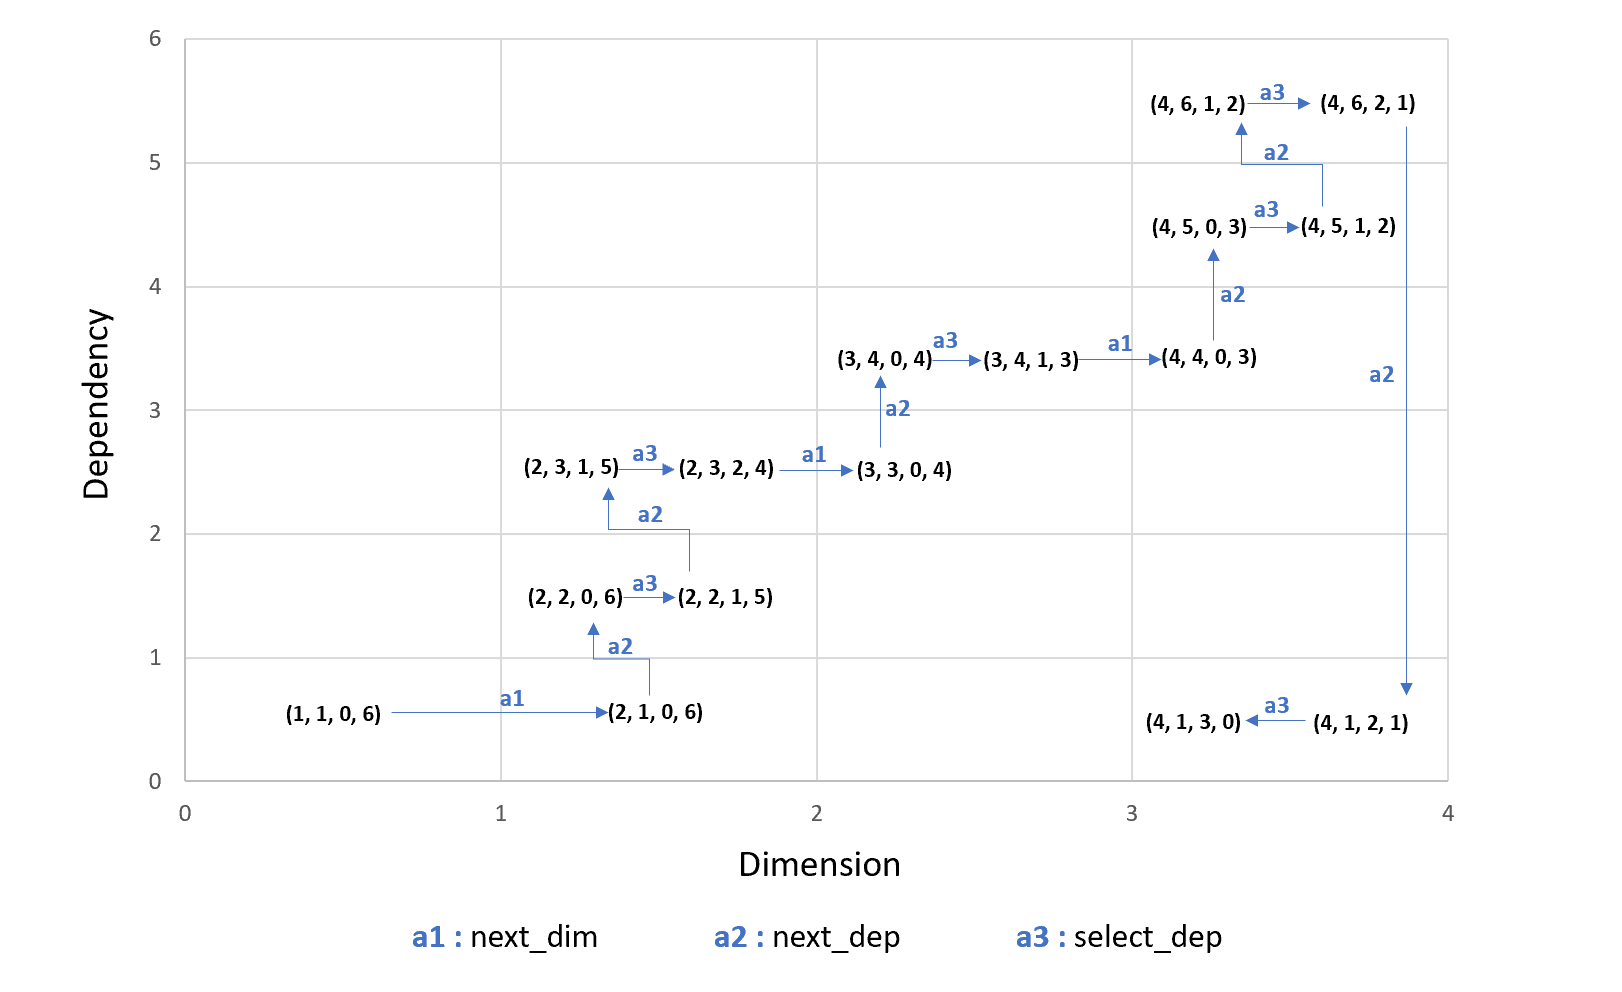
\includegraphics[width=\textwidth]{Images/Construction.png}    
  \caption{Construction Phase State Representation as \textit{(i_{dim};\hspace{2}i_{dep};\hspace{2}n_d;\hspace{2}n_a)}.}
  \label{fig:construction}
\end{figure}

Using this representation, the agent could learn if trained and tested on the same kernel. Just within 20 iterations, we achieved an impressive speedup,  even better than the best speedup acquired during the training. While this shows that the agent's implementation is correct, more work was needed to solve the problem of generalisation. While testing this agent on another kernel, the performance was significantly poor.

A critical piece of information we included was the actual parameters associated with the dependency. A dependency statement can be defined as shown below.
\begin{equation}
\begin{multlined}
[n_i, \hspace{2} n_j, \hspace{2} n_k] \hspace{2} -> \hspace{2} Stmt\_for\_body8[i_0, \hspace{2} i_1] -> Stmt\_for\_body16[i_0', \hspace{2} i_1', \hspace{2} i_2] : \\
i_0' = i_0 \hspace{2} and \hspace{2} i_1' = 0 \hspace{2} and \hspace{2} i_2 = i_1 \hspace{2} and \hspace{2} n_k > 0 \hspace{2} and \hspace{2} 0 <= i_0 < n_i \hspace{2} and \hspace{2} 2i_1<=i_0
\label{eq:DEP_STMT}
\end{multlined}
\end{equation}

The dependency defined in \ref{eq:DEP_STMT} consists of \textit{domain} variables, \textit{statements} and variable bounds, which can be presented as affine functions. To provide all the inequalities of a regular structure, we converted all the expressions in the format of less than equal to zero.
For example, \textit{$0 \leq \hspace{2}$i\textsubscript{0} $< \hspace{2}$n\textsubscript{i}}  can be transformed to two different affine functions \textit{$-i\textsubscript{0} \leq \hspace{2}$0} and \textit{$i\textsubscript{0} - \hspace{2}n\textsubscript{i} + 1 \leq \hspace{2}$0}. We are allowing dependencies having four variables and four domain parameters. 
Hence we can have four variables \textit{$i_0, \hspace{2} i_1, \hspace{2} i_2, \hspace{2} i_3$}, four prime variables for the second statement \textit{$i_0', \hspace{2} i_1', \hspace{2} i_2', \hspace{2} i_3'$}, four domains \textit{$n_i, \hspace{2} n_j, \hspace{2} n_k, \hspace{2} n_m$} and one constant. Thus, inequality can be expressed in terms of the vector as shown below.\break
\begin{center}
\textit{$i\textsubscript{0} - \hspace{2}n\textsubscript{i} + 1 \leq \hspace{2}$0} \hspace{4} \verb|->| \hspace{4} [1 0 0 0 0 0 0 0 -1 0 0 0 1]
\end{center}

If we allow such eight inequalities in one dependency statement, the number of variables representing the statement will be 13 * 2 * 8 = 208.

The last two parameters of the state representation, the number of strong dependencies added in the current dimension and the number of available dependencies to be added, also presented a few challenges. Firstly, they do not contain the information on which dependency was added strongly and which is yet to be added. Secondly, the number of dependencies could be as high as more than 80 in the kernels such as \textit{ludcmp}. Hence, we used one-hot encoding to state the added and available dependencies. For instance, if the maximum number of dependencies considered is 10, the dependencies added in the current dimension can be defined as:

\begin{center}
[1 0 0 0 1 1 0 0 0 0],
\end{center}

The above vector showcases that dependency numbers 1, 5, and 6 are added strongly in the current dimension. Similarly, to define available dependencies, we use vector
\begin{center}
[0 1 0 0 0 0 0 0 1 1],
\end{center}

Which states that dependencies 2, 9, and 10 are still not added strongly in any dimension and are still available to be added. We have considered the kernels having a maximum number of dependencies of 41, due to the higher construction time for the kernels having dependencies more than that. Hence, this adds 82 more variables to our state representation, taking the total variable count, including the current dimension, to 1 + 208 + 82 = 291. We have mixed and matched these representation variables, implementing dropouts, for example, using the number of available dependencies instead of one-hot encoding to determine which representation gives us the best result. A typical full expression of the state would look as shown below.

\textit{array([ 0.,  0.,  0.,  0.,  0.,  0.,  0.,  0.,  0.,  0., -1.,  0.,  0.,
        1.,  0.,  0.,  0.,  0.,  0.,  0.,  1.,  0.,  0., -1.,  0.,  0.,
        0.,  0.,  0.,  0.,  0.,  0.,  0.,  0.,  1.,  0.,  0.,  0.,  0.,
        0.,  0.,  0.,  0.,  0., -1.,  0.,  0.,  0.,  0., -1.,  0., -1.,
        1.,  0.,  0.,  0.,  0.,  0.,  0.,  0.,  0.,  1., -1.,  0.,  0.,
        0.,  0.,  0.,  0.,  0.,  0.,  0.,  0.,  0.,  0.,  0.,  0.,  0.,
       -1.,  1., -1.,  0.,  0.,  0.,  0.,  0.,  0.,  0.,  0., -1.,  1.,
        0.,  0.,  0.,  0.,  0., -1.,  0.,  0.,  1., -1.,  2.,  0.,  0.,
        0.,  0.,  0.,  0.,  0.,  0.,  0.,  0.,  0.,  0.,  0.,  0.,  0.,
        0.,  0.,  0.,  0.,  0.,  0.,  0.,  0.,  0.,  0.,  0.,  0.,  0.,
        0.,  0.,  0.,  0.,  0.,  0.,  0.,  0.,  0.,  0.,  0.,  0.,  0.,
        0.,  0.,  0.,  0.,  0.,  0.,  0.,  0.,  0.,  0.,  0.,  0.,  0.,
        0.,  0.,  0.,  0. ......])}

%\textit{0 \leq i\textsubscript{0} < n\textsubscript{i}}
%\textit{-i\textsubscript{0} \leq 0}
%\textit{i\textsubscript{0} - n\textsubscript{i} + 1 \leq 0}
\subsection{Exploration Phase}

The exploration phase inputs the list of generators defined in the construction phase and returns a point in each dimension in the polytope of the schedule. This point is generated by selecting a coefficient and applying it to the corresponding term of the generator. Thus, the searching problem becomes the problem of finding the proper integer coefficients to apply to the terms. Hence, for the exploration of schedule space, the action space consists of three actions as defined in Equation \ref{eq:CONST_ACT},
\begin{equation}
A_{con} = \{select\_coeff0, \hspace{1} select\_coeff1, \hspace{1} select\_coeff2\}
\label{eq:EXP_ACT}
\end{equation}

The point generated for each dimension might look like as shown below.
p_1 = (0,0,0,-1,0,0,0) + 2.(0,1,0,0,0,0,-1) 
 (0,0,-1,-1,0,0,0) + 2.(-1,0,0,10,0,0,0)

Notably, once the point is generated, we multiply it with the least common denominator(LCD) to ensure the point is in lattice polytope and we have a valid schedule.

Initially, for the state representation, we included only the dimension of the polytope taken from the set of polytopes and the current term we are working on. However, it is crucial to consider that a good schedule depends on the combination of the coefficients selected for the current term, other terms in the same dimension, and all the terms determined in other dimensions. Hence, only the information about the current term may not be enough. This concept is explained in Figure \ref{fig:exploration}. As shown, in the case of Ray2, whether to select coeff0 or coeff1 for a good schedule will depend on what is already selected for Ray1. In this example, we have taken just two rays for understanding. In an actual scenario, this behaviour also extends to selection in other terms and dimensions. Hence, the state representation was expanded to include the points generated until that point during the exploration. A typical state representation for d polytopes during the exploration is shown in Equation \ref{eq:EXPL_SPC}.

\begin{equation}
S_{expl} = (i_{d} ;\hspace{2} current\_term;\hspace{2} p_1,....p_d;)
\label{eq:EXPL_SPC}
\end{equation}

\begin{figure}[htbp]
  \centering
  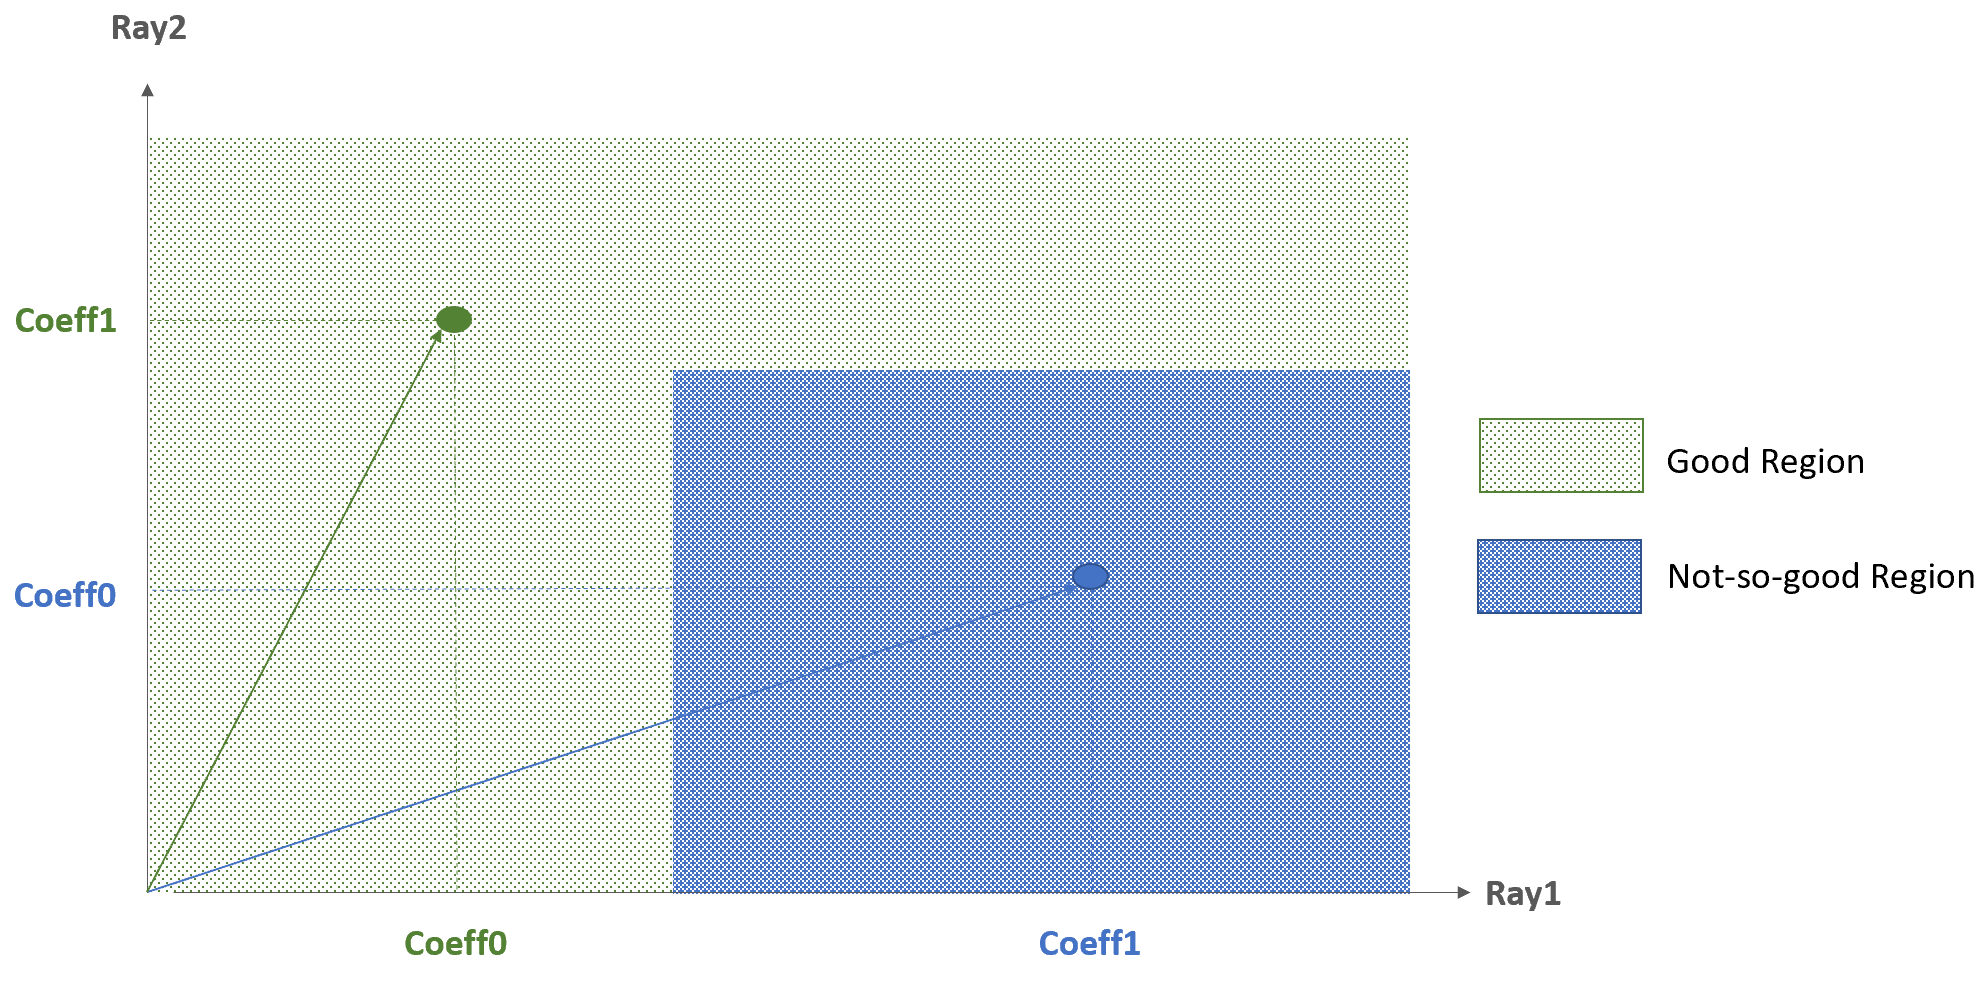
\includegraphics[width=\textwidth]{Images/Exploration.png}    
  \caption{Exploration Phase limited to one dimension and two rays for understanding}
  \label{fig:exploration}
\end{figure}

\begin{figure}[!tb]
  \centering
  \subfloat[Original Loop in C.]{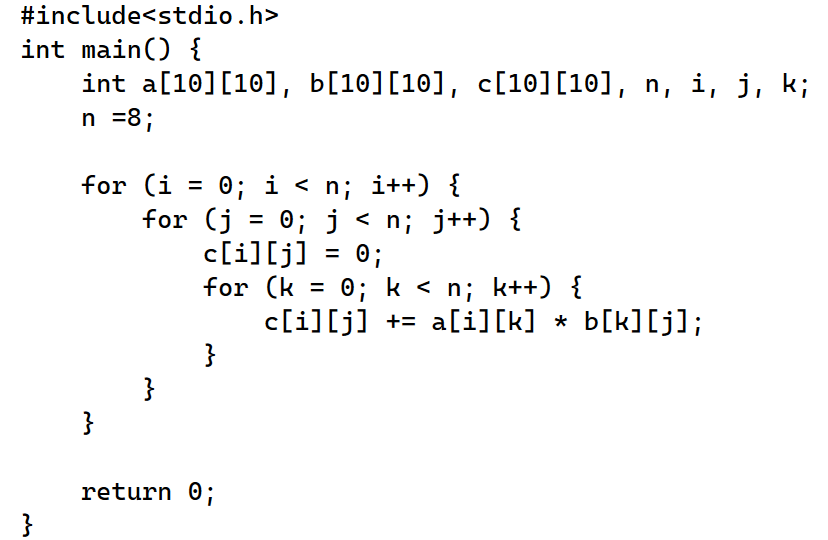
\includegraphics[width=0.5\textwidth]{Original_Loop.png}\label{fig:Original_Loop}}
  \hfill
  \subfloat[Polyhedral Representation of the identified SCoP.]{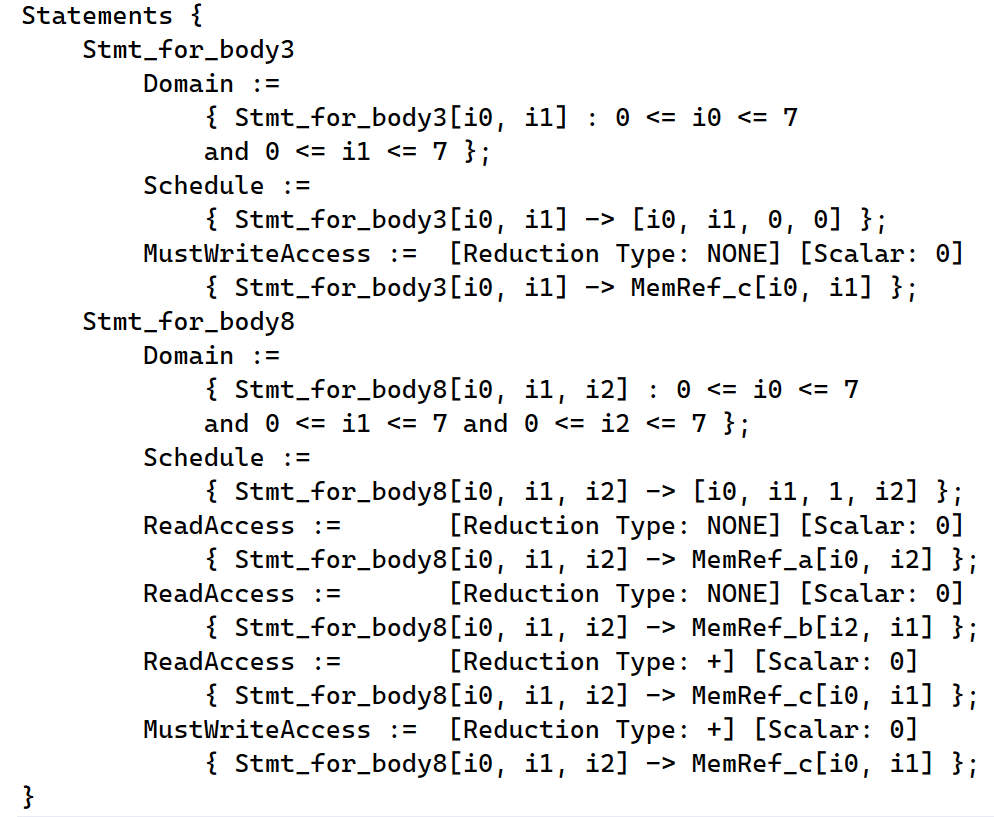
\includegraphics[width=0.5\textwidth]{Poly_Rep.png}\label{fig:Poly_Rep}}

  \centering
  \subfloat[Dependency Analysis.]{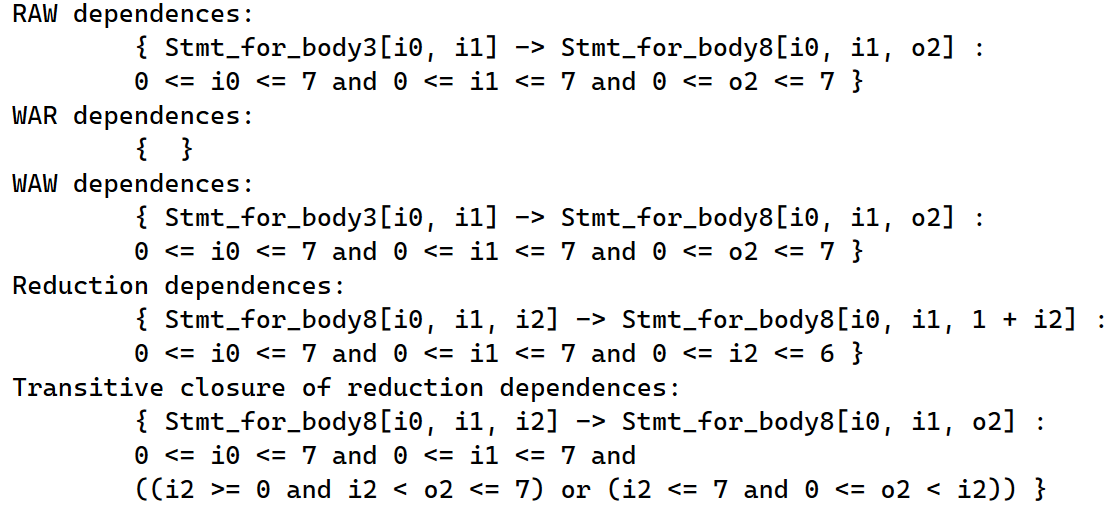
\includegraphics[width=0.5\textwidth]{Dependencies.png}\label{fig:Dependencies}}
  \hfill
  \subfloat[AST Generation from IR.]{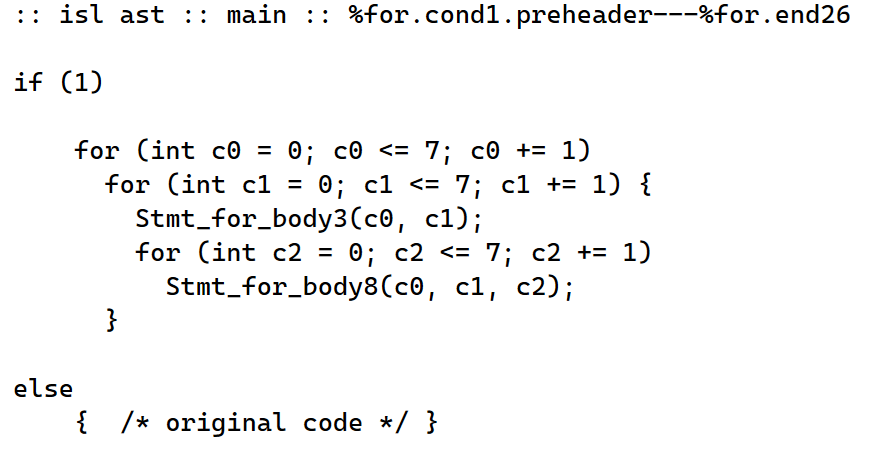
\includegraphics[width=0.5\textwidth]{AST.png}\label{fig:AST}}
  
  \caption{Generation of SCoP and AST using LLVM Polly}
\end{figure}

\section{Epsilon-Greedy Approach}

During the training, the agent has two choices. Either keep choosing the new actions, which is called exploration or choose the actions giving the most reward, termed exploitation. Exploration is good for the long run as the agent gains new knowledge. While exploitation helps earn immediate rewards, even though it might be sub-optimal. The agent can follow only one approach at a time, presenting an exploration-exploitation trade-off. In the implementation, a parameter \textit{epsilon} was kept to introduce the randomness in the training. We choose a random number from 0 to 1. If the number is less than \textit{epsilon}, then the agent explores, or else it exploits, Figure \ref{fig:randomness}.

\begin{figure}[htbp]
  \centering
  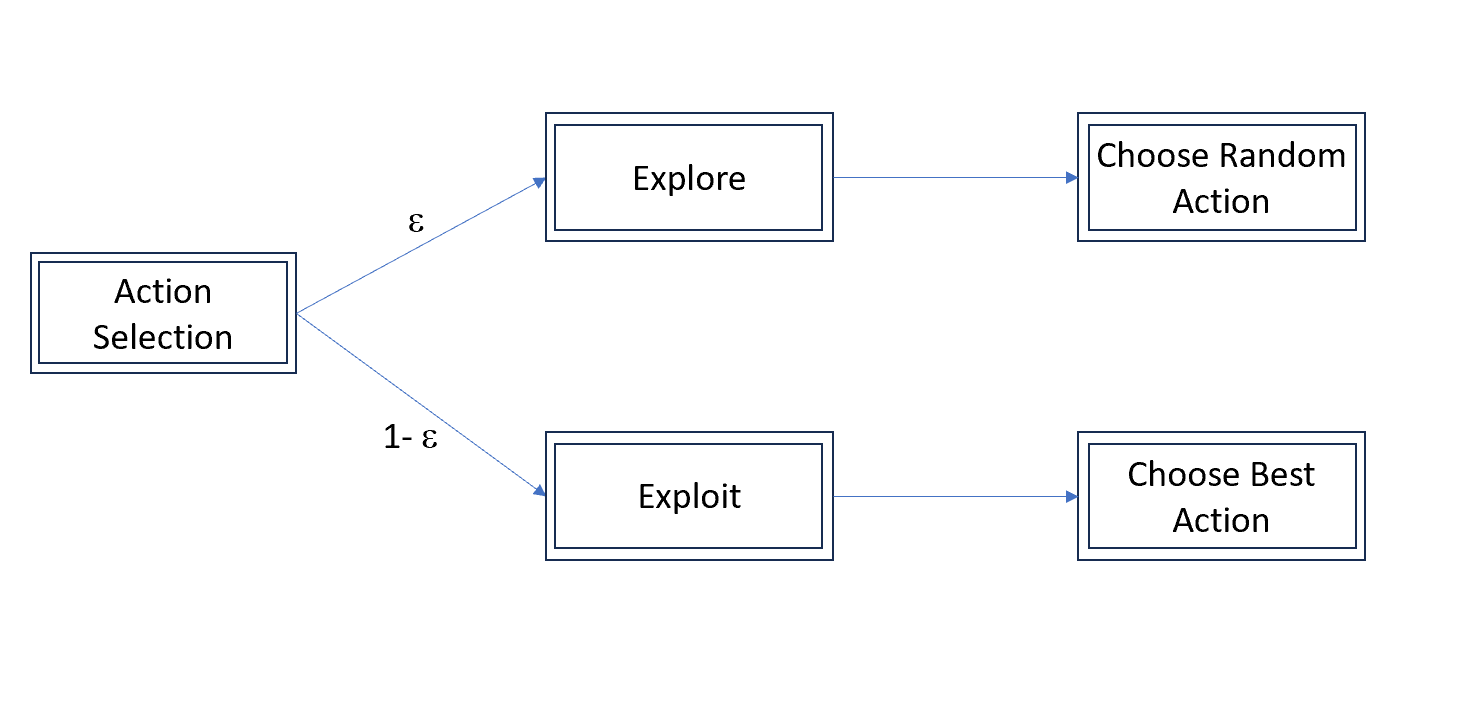
\includegraphics[width=\textwidth]{Images/Randomness.png}    
  \caption{Exploration vs Exploitation}
  \label{fig:randomness}
\end{figure}

Initially, the agent has little information and needs to explore more. Hence, the value of \textit{epsilon} should be higher. As the training progresses, this value should be reduced so that the agent does not spend time on actions which will not give us good rewards. However, the randomness should be decreased periodically. Otherwise, more exploitation in the initial phase can cause the agent to get stuck in sub-optimal space. We are reducing the \textit{epsilon} value based on the iteration of the training as described in Equation \ref{eq:RANDOMNESS}. Notably, if {$\epsilon$} value is zero, the agent always exploits the knowledge it has. Conversely, the agent will always choose random actions if the {$\epsilon$} value is one.


\begin{equation}
\epsilon = 1.0 - (min{\hspace{2}}(1.0,{\hspace{2}} t / (0.9 * T))) * {\hspace{2}}0.95
\label{eq:RANDOMNESS}
\end{equation},

where t is the current iteration, and T is the total number of iterations for the training.

\section{Experience Replay Buffer}
Instead of learning as soon as we take a step in the environment, we store these transitions in a memory buffer, which can be utilised later on for learning purposes. This is known as learning based on Experience Replay in Reinforcement learning\cite{ER}. This approach has many advantages. Firstly, we need a good way to distribute the reward to all the state-actions pairs visited during the scheduled construction and exploration. However, we can do this only once we know the speed-up of the new schedule generated. Navigating the transition history, we update the values for those state-action pairs later. Secondly, if we plan to train on each kernel n times, we can pick one kernel train for n times and move to the next kernel. However, this approach might introduce some correlation in the learning. If we store the transition history, we can randomly select the samples to break the correlation\cite{RAMICIC202091}.

The base unit of this replay buffer is a transition, which can be described as per Equation \ref{eq:TRANSITION}

\begin{equation}
T = (s,\hspace{2} a,\hspace{2} r,\hspace{2} s,\hspace{2} d),
\label{eq:TRANSITION}
\end{equation}

where \textit{T} is Transition, \textit{s} is the current state in which the action is taken, \textit{a} is the action performed, \textit{r} is the reward received while performing action \textit{a} in states \textit{s}, \textit{s'} is the next state in the transition and \textit{d} is the binary value to indicate if the transition is completed, which is if the schedule is generated.

\chapter{Evaluation and Results}

\section{Evaluation Setup}

PolyGym builds atop Polyite [https://stganser.bitbucket.io/taco2017/], which is a tool to iteratively optimize the program's schedule to increase its performance on multi-core systems. Polyite uses a patched version of Polly to extract Scop and generate the transformed code from the schedule. Polly is built on top of LLVM. Hence, as a first step of the set-up, LLVM[reference to be added], clang and Polly were cloned and built using \textit{cmake}. The next step was building isl[reference to be added] and its binding for Scala 2.11. A wrapper is used to make these isl Scala binding available to Polyite\cite{10.1145/3109482}. Next, two libraries Barvinok\cite{10.5555/261410.261418} and Chernikova\cite{leverge:inria-00074895} were set up. The former calculates the polyhedron's volume, while the latter generates the generator representation from linear constraints. As there is no build tool supplied with Polyite, all the required libraries, such as Apache Commons Lang 3.4, Apache Commons Math 3.6.1, OpenMPI 2.1.1\cite{OpenMPI}, scala-parser-combinators 2.11-1.0.3 were added as dependencies to Scala IDE[reference] to build the tool. Finally, PolyBench version 4.1 was downloaded and unpacked inside Polyite root location. The stack hierarchy is shown in Figure \ref{fig::stack}.

\begin{figure}[htbp]  
  \centering
  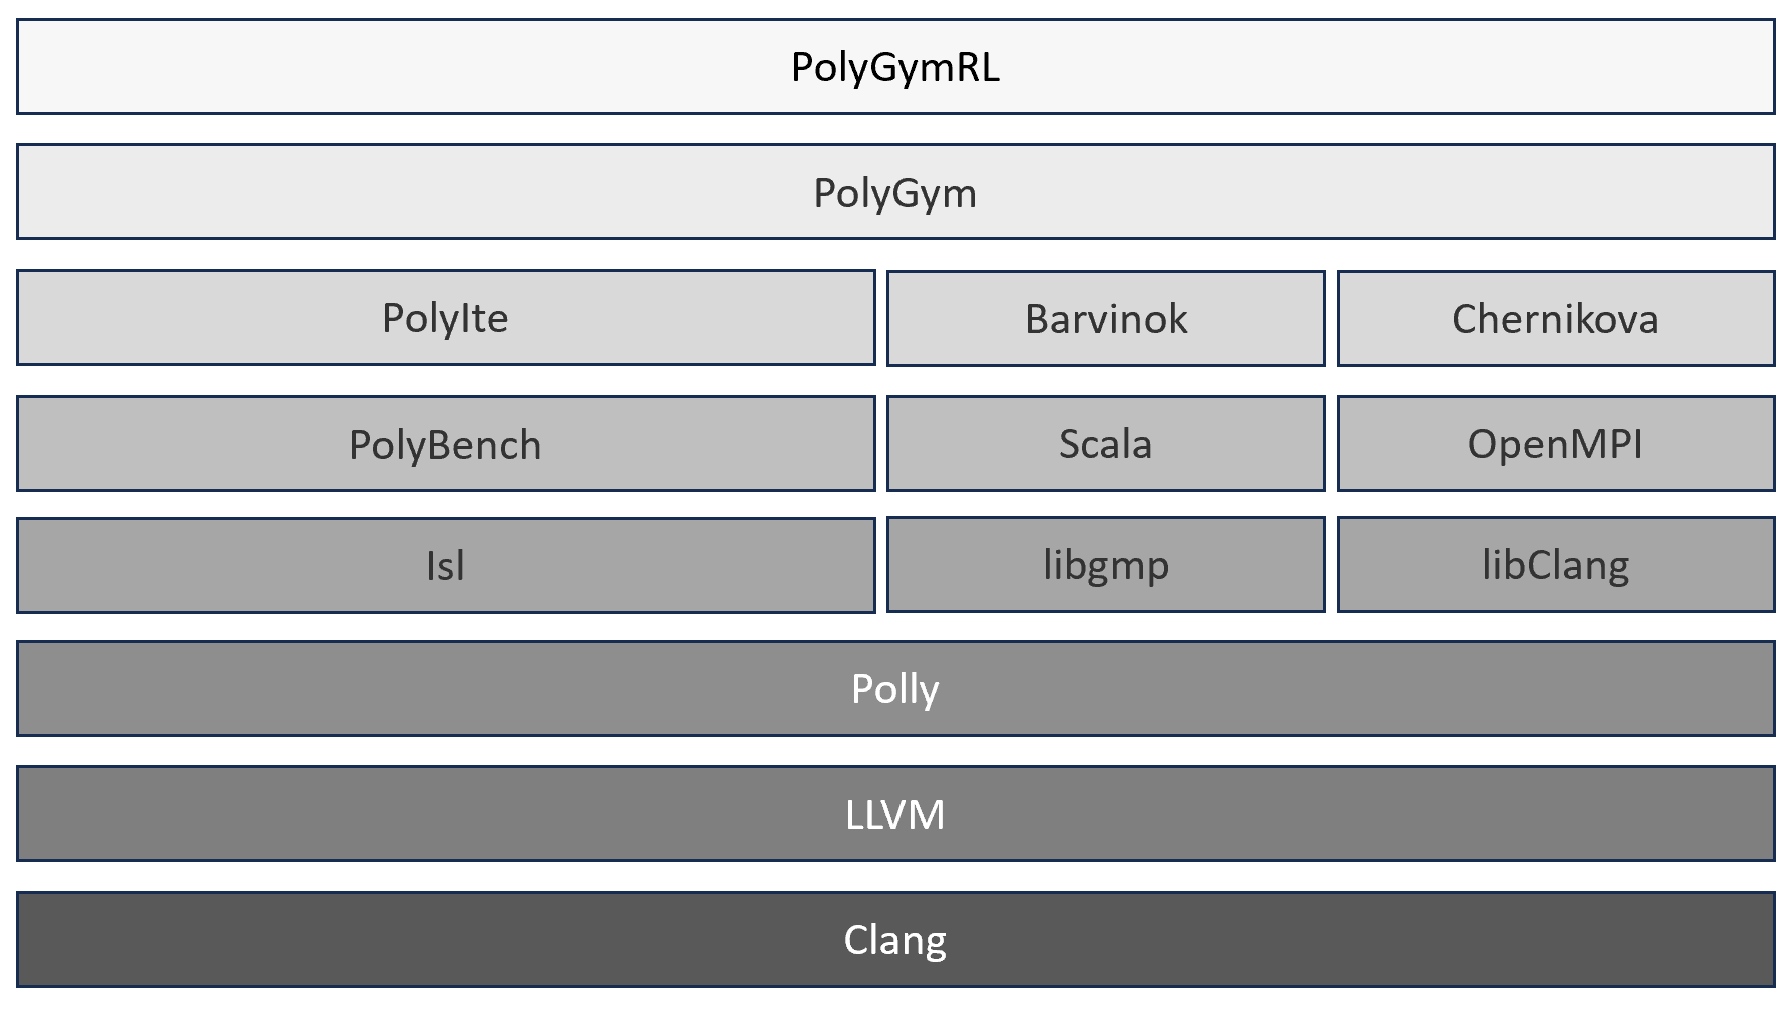
\includegraphics[width=\textwidth]{Images/PolyGymRlStack.png}    
  \caption{PolyGymRL Stack}
  \label{fig::stack}
\end{figure}



\section{Leave-one-out Evaluation}

We have conflicting priorities while distributing training and testing sets. Our training set should be large enough for the agent to learn correctly. Conversely, our testing set should be large enough to accurately measure our agent's performance. One approach to finding a middle way is to perform cross-validation, where we train and test our algorithm on the same data multiple times. We first train the agent on the training set and measure the performance on the testing set. On the next iteration, we flip the sets, train the agent on the set used for testing and test it on the remaining set. In practice, there are generally more than two partitions; we take a different partition each time for testing. In the end, we take an average of the performance of each instance. In this case, for n number of kernel examples, we tested the agent on one loop kernel after training it on n-1 kernels. Each time leave one kernel out and train the agent on other kernels, which is similar to the Leave-One-Out evaluation method\cite{inbook}. This way, our agent is exposed to the most learning, although it has increased the overall computation significantly. This method is shown in Figure \ref{fig:leave_one_out} with the help of five different kernels; however, there were more than five kernels during the actual evaluation.

\begin{figure}[htbp]
  \centering
  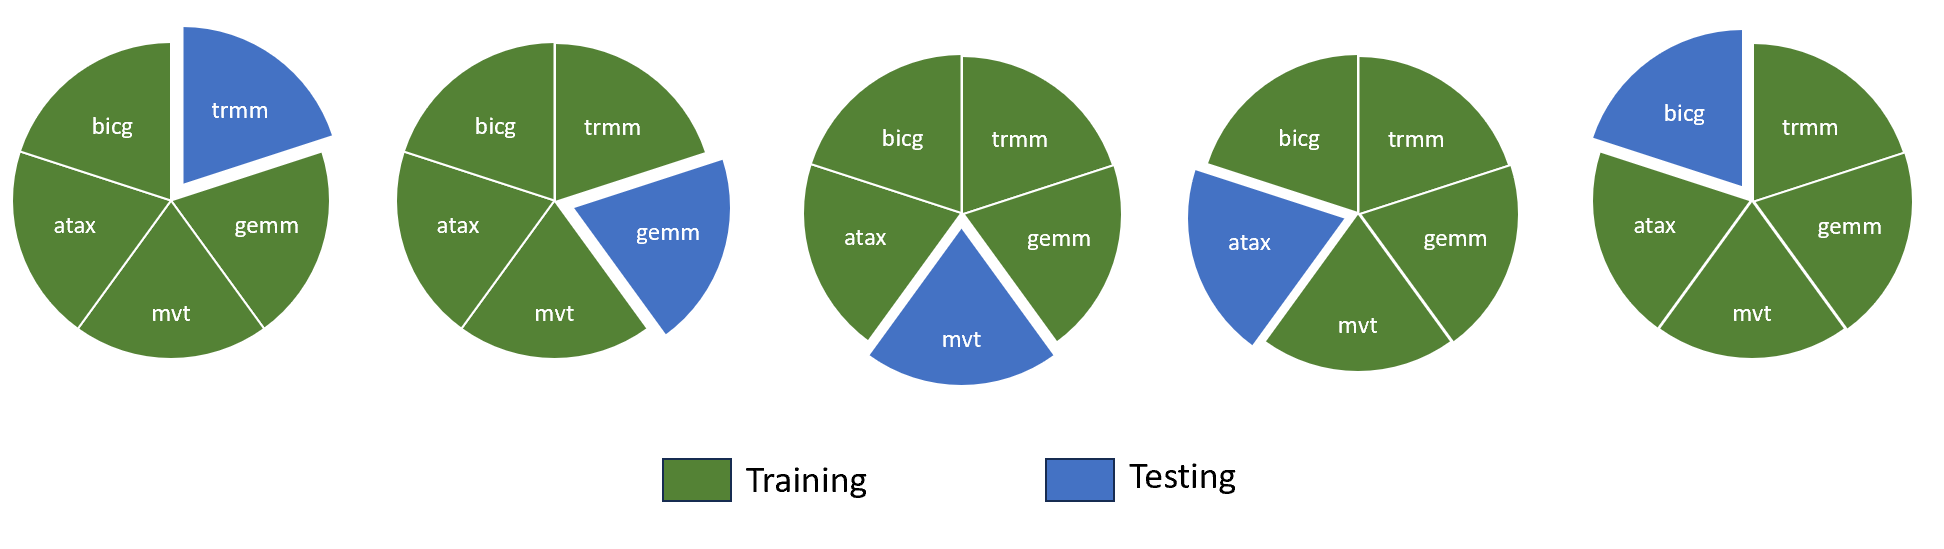
\includegraphics[width=\textwidth]{Images/Leave_One_Out.png}   
  \caption{Leave-One-Out Evaluation}
  \label{fig:leave_one_out} 
\end{figure}

\Section{Results}
 We are trying to answer two major questions by undertaking this study. The first question is how is PolyGymRL faring compared to the original PolyGym implementation. The next question is related to comparing the difference between the performance of different algorithm variations. As a basic primary check, we are comparing the single kernel performance of PolyGym with PolyGymRL, meaning we are performing the test on the same loop we used during the training. In this case, we expect to yield higher speedups as no generalisation is involved. The comparison of single kernel performance of PolyGym and PolyGymRL is shown in Figure \ref{fig:single_PolyGym_PolyGymRL}. As no training is involved in PolyGym, the heuristics can yield different results each time.  In the case of PolyGYmRL, we have trained the agent on a kernel for 12 iterations. We test both implementations for three iterations and take the geometric mean of the results. Notably, the original PolyGym research paper listed the best result, while here we are considering the geometric mean values; hence both research findings are not directly comparable, especially as it is heavily based on randomness. For the second experiment, as shown \ref{fig:multi_PolyGym_PolyGymRL}, we work with different sets of kernels in training and testing, using leave-one-out evaluation. From both charts, it can be seen that PolyGymRL reported better speedups thanks to the learning of the agent. From this data, we can also see that when we work with different sets of kernels in training and testing, the acquired speedup does not match the standards of single-loop training as it is often in the case of generalisation.

\begin{figure}[htbp]
  \centering
  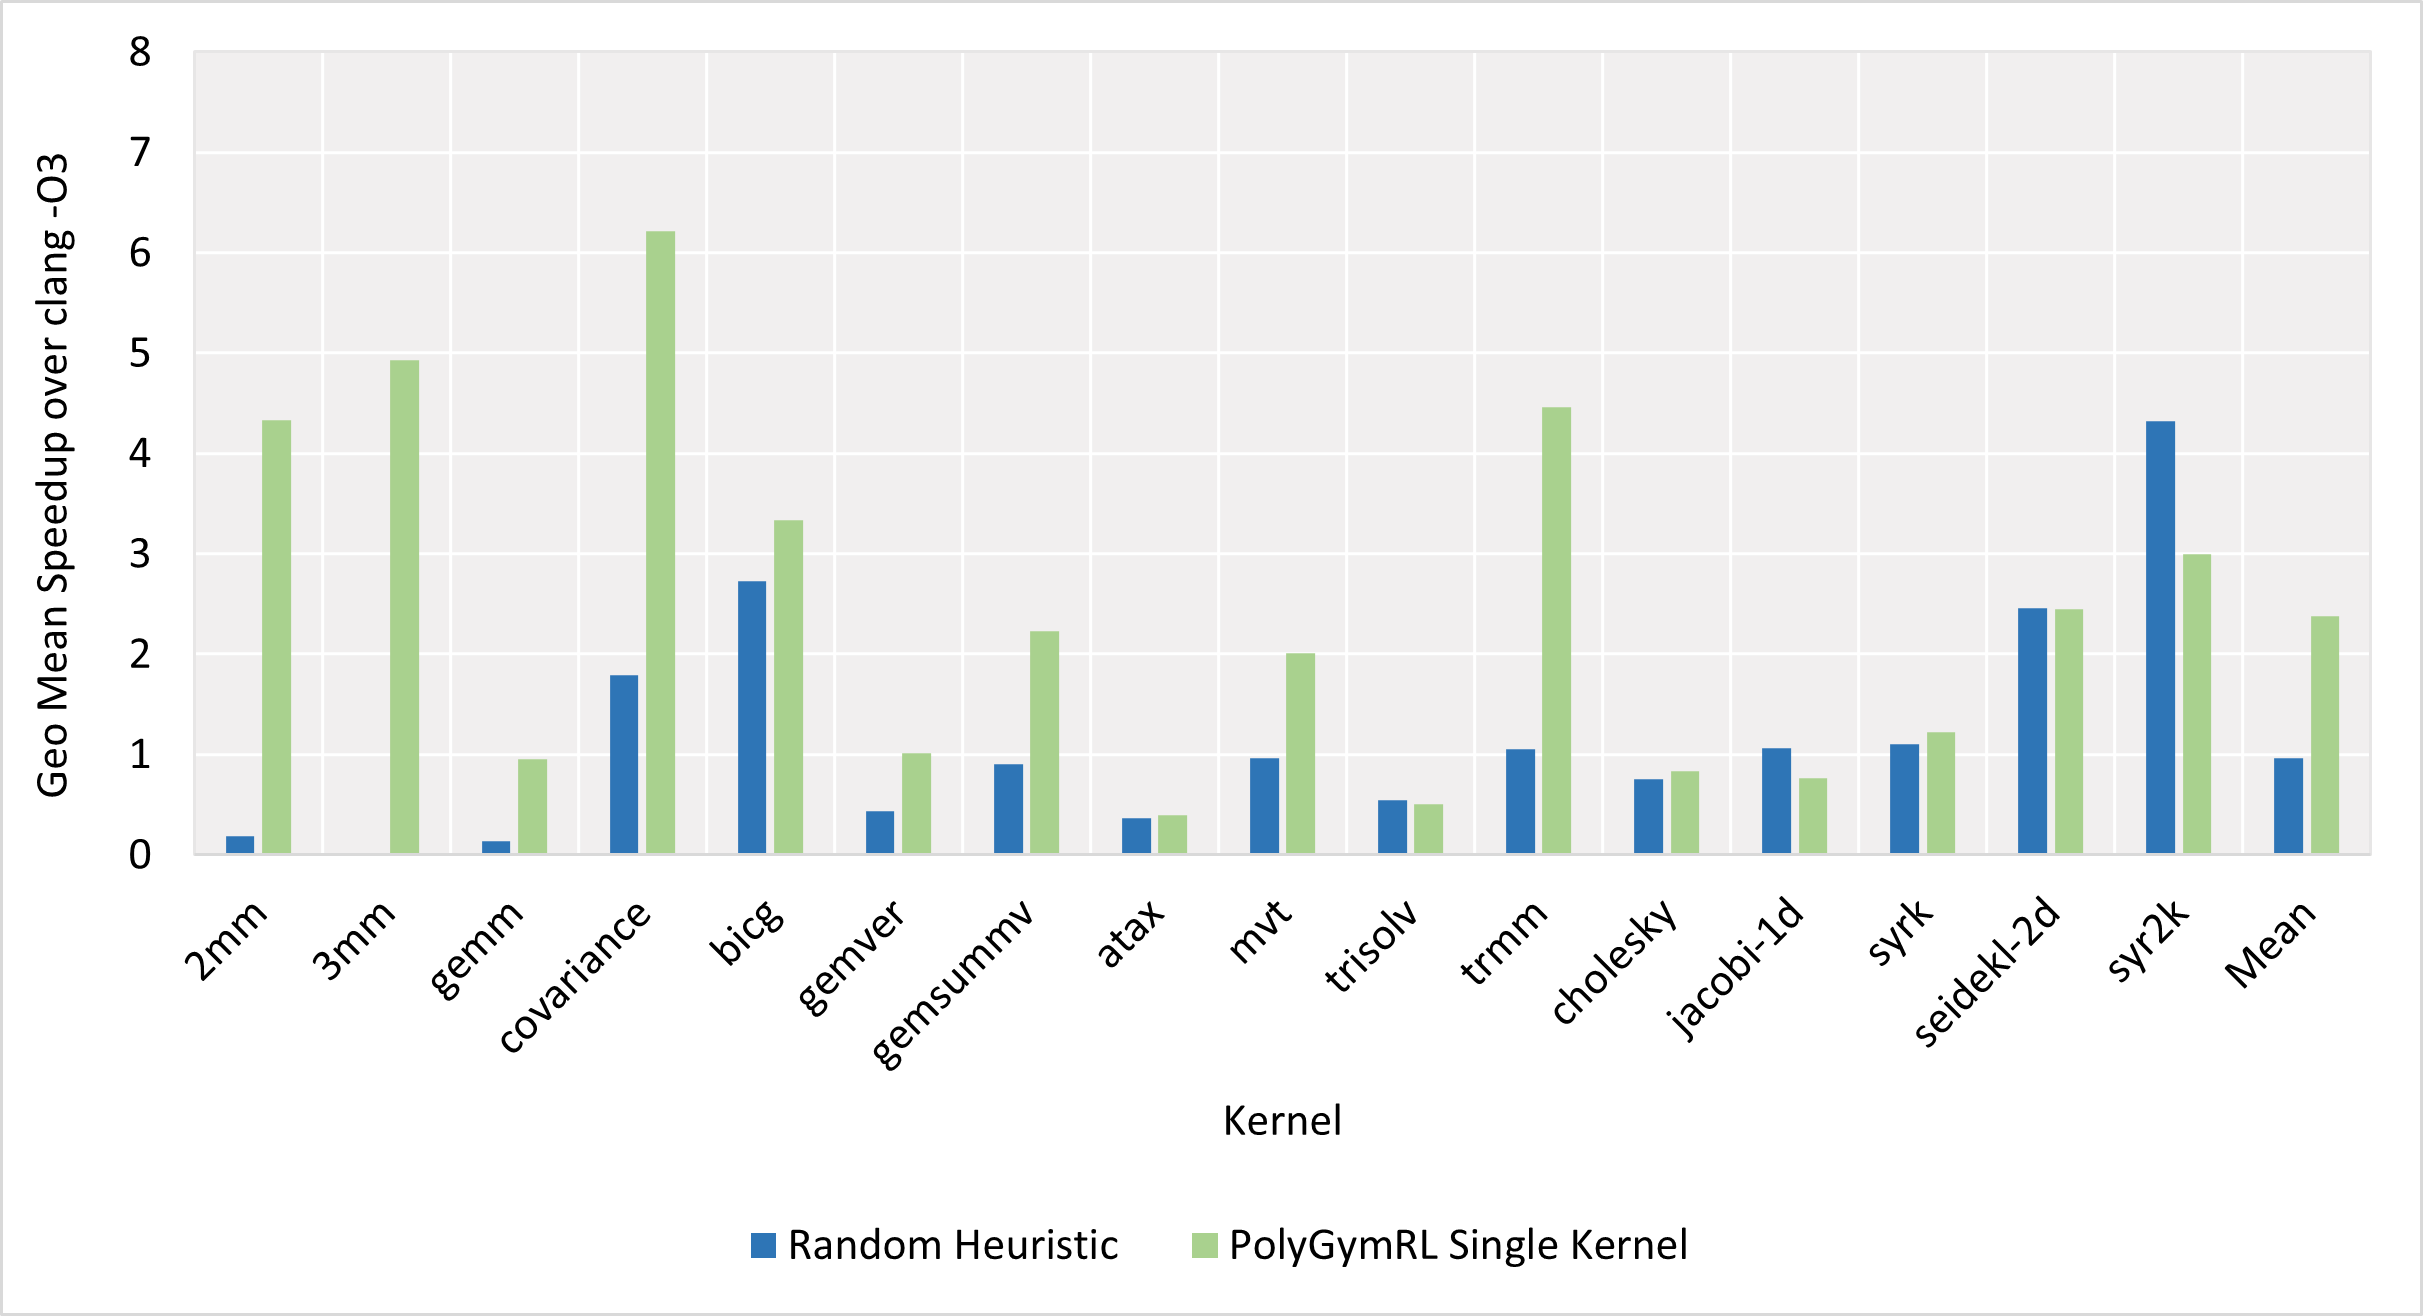
\includegraphics[width=0.75\textwidth]{Images/Chart_Single_PolyGym_PolyGymRL.png}    
  \caption{Comparison of Average Speedup achieved in PolyGym and PolyGymRL while training and testing on the same kernel}
  \label{fig:single_PolyGym_PolyGymRL}
\end{figure}

\begin{figure}[htbp]
  \centering
  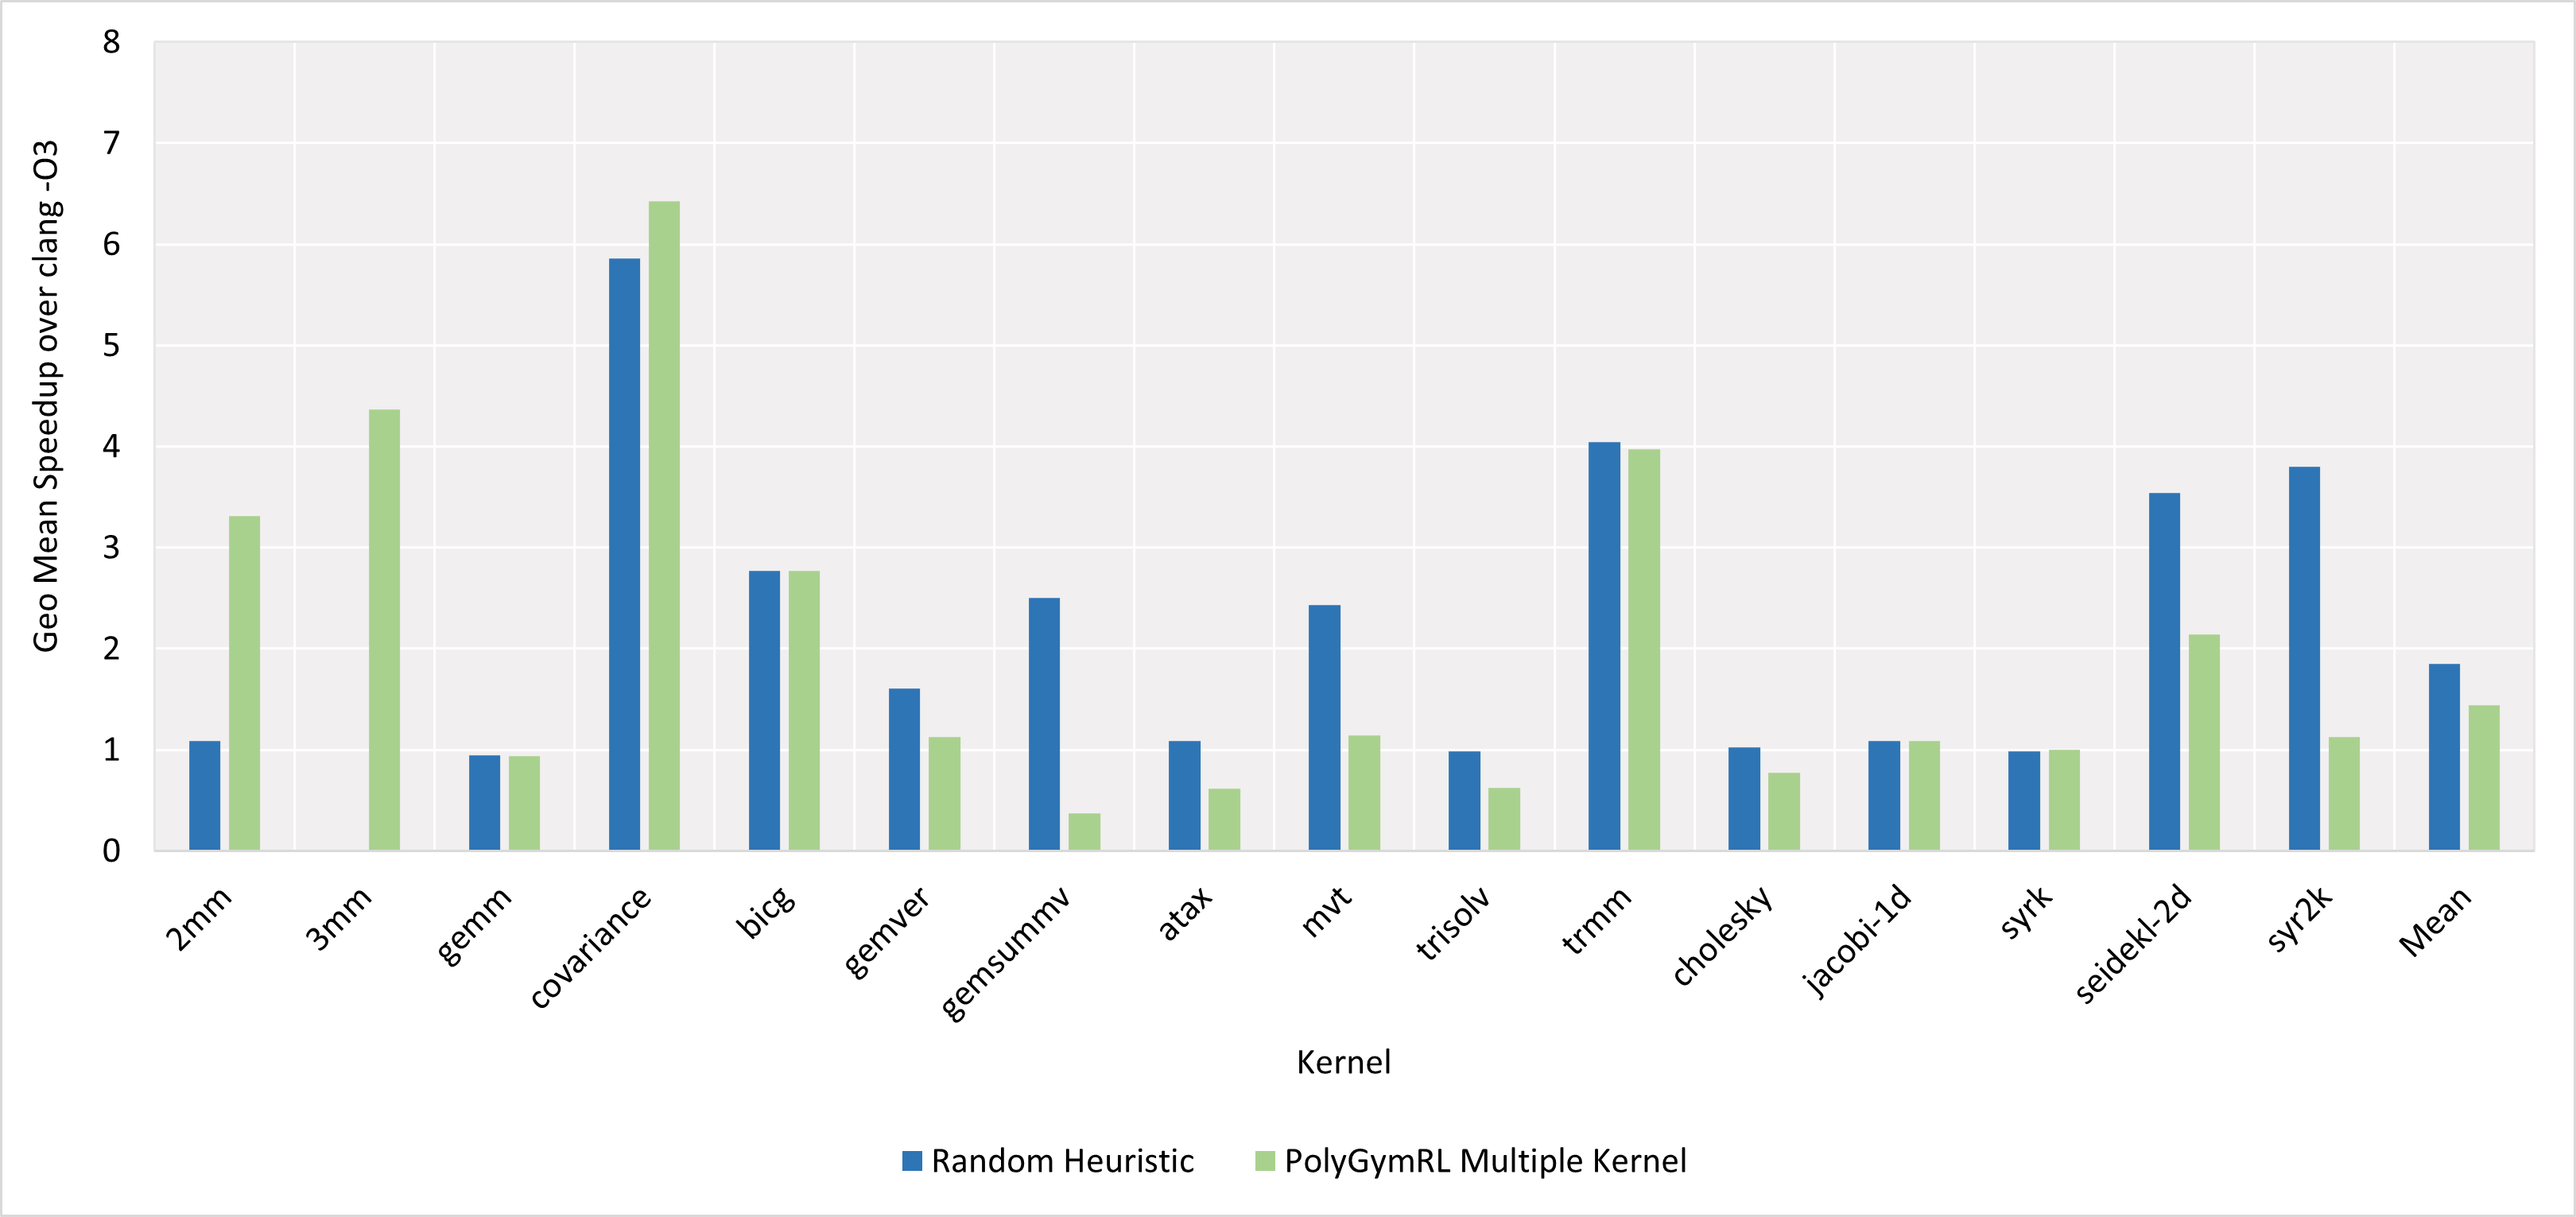
\includegraphics[width=0.75\textwidth]{Images/Chart_Multiple_PolyGym_PolyGymRL.png}    
  \caption{Comparison of Average Speedup achieved in PolyGym and PolyGymRL using Leave-One-Out Evaluation}
  \label{fig:multi_PolyGym_PolyGymRL}
\end{figure}

If we now turn to our next analysis, we compare the results of PolyGymRL for various strategies and configurations. We have mainly considered three factors: standardisation, representation and bias. Figure \ref{fig:Std_Chart} and Figure \ref{fig:NoStd_Chart} presents the mean speedups obtained for different PolyBench kernels with or without applying the standardisation. How we have applied the standardisation is explained in more detail in \ref{sec:std}. The last data on the horizontal axis corresponds to the average taken across all the kernels for the respective strategy. The average speedups for the strategies involving standardisation yields 1.23x better performance than those without standardisation. Moving now to the experimental evidence on the effect of keeping simple or full representation, the results can be seen in \ref{fig:Simple_Chart} and \ref{fig:NoSimple_Chart}. The agents seem to utilise the detailed information provided in the full representation to make better decisions. Figure \ref{fig:Bias_Chart} and Figure \ref{fig:NoBias_Chart} compare the results obtained while keeping bias for action \textit{select\_coeff0} during exploration versus otherwise. The difference between both strategies was significant, as selecting lower coefficients might help find the less complex schedules. A comparison among all these strategies is provided in Figure \ref{fig:PolyGymRL_Versions}. There are also some more comparison charts included in the Appendix Section \ref{sec:Compare_Versions}.

\begin{figure}
\centering
\begin{minipage}{.45\linewidth}
  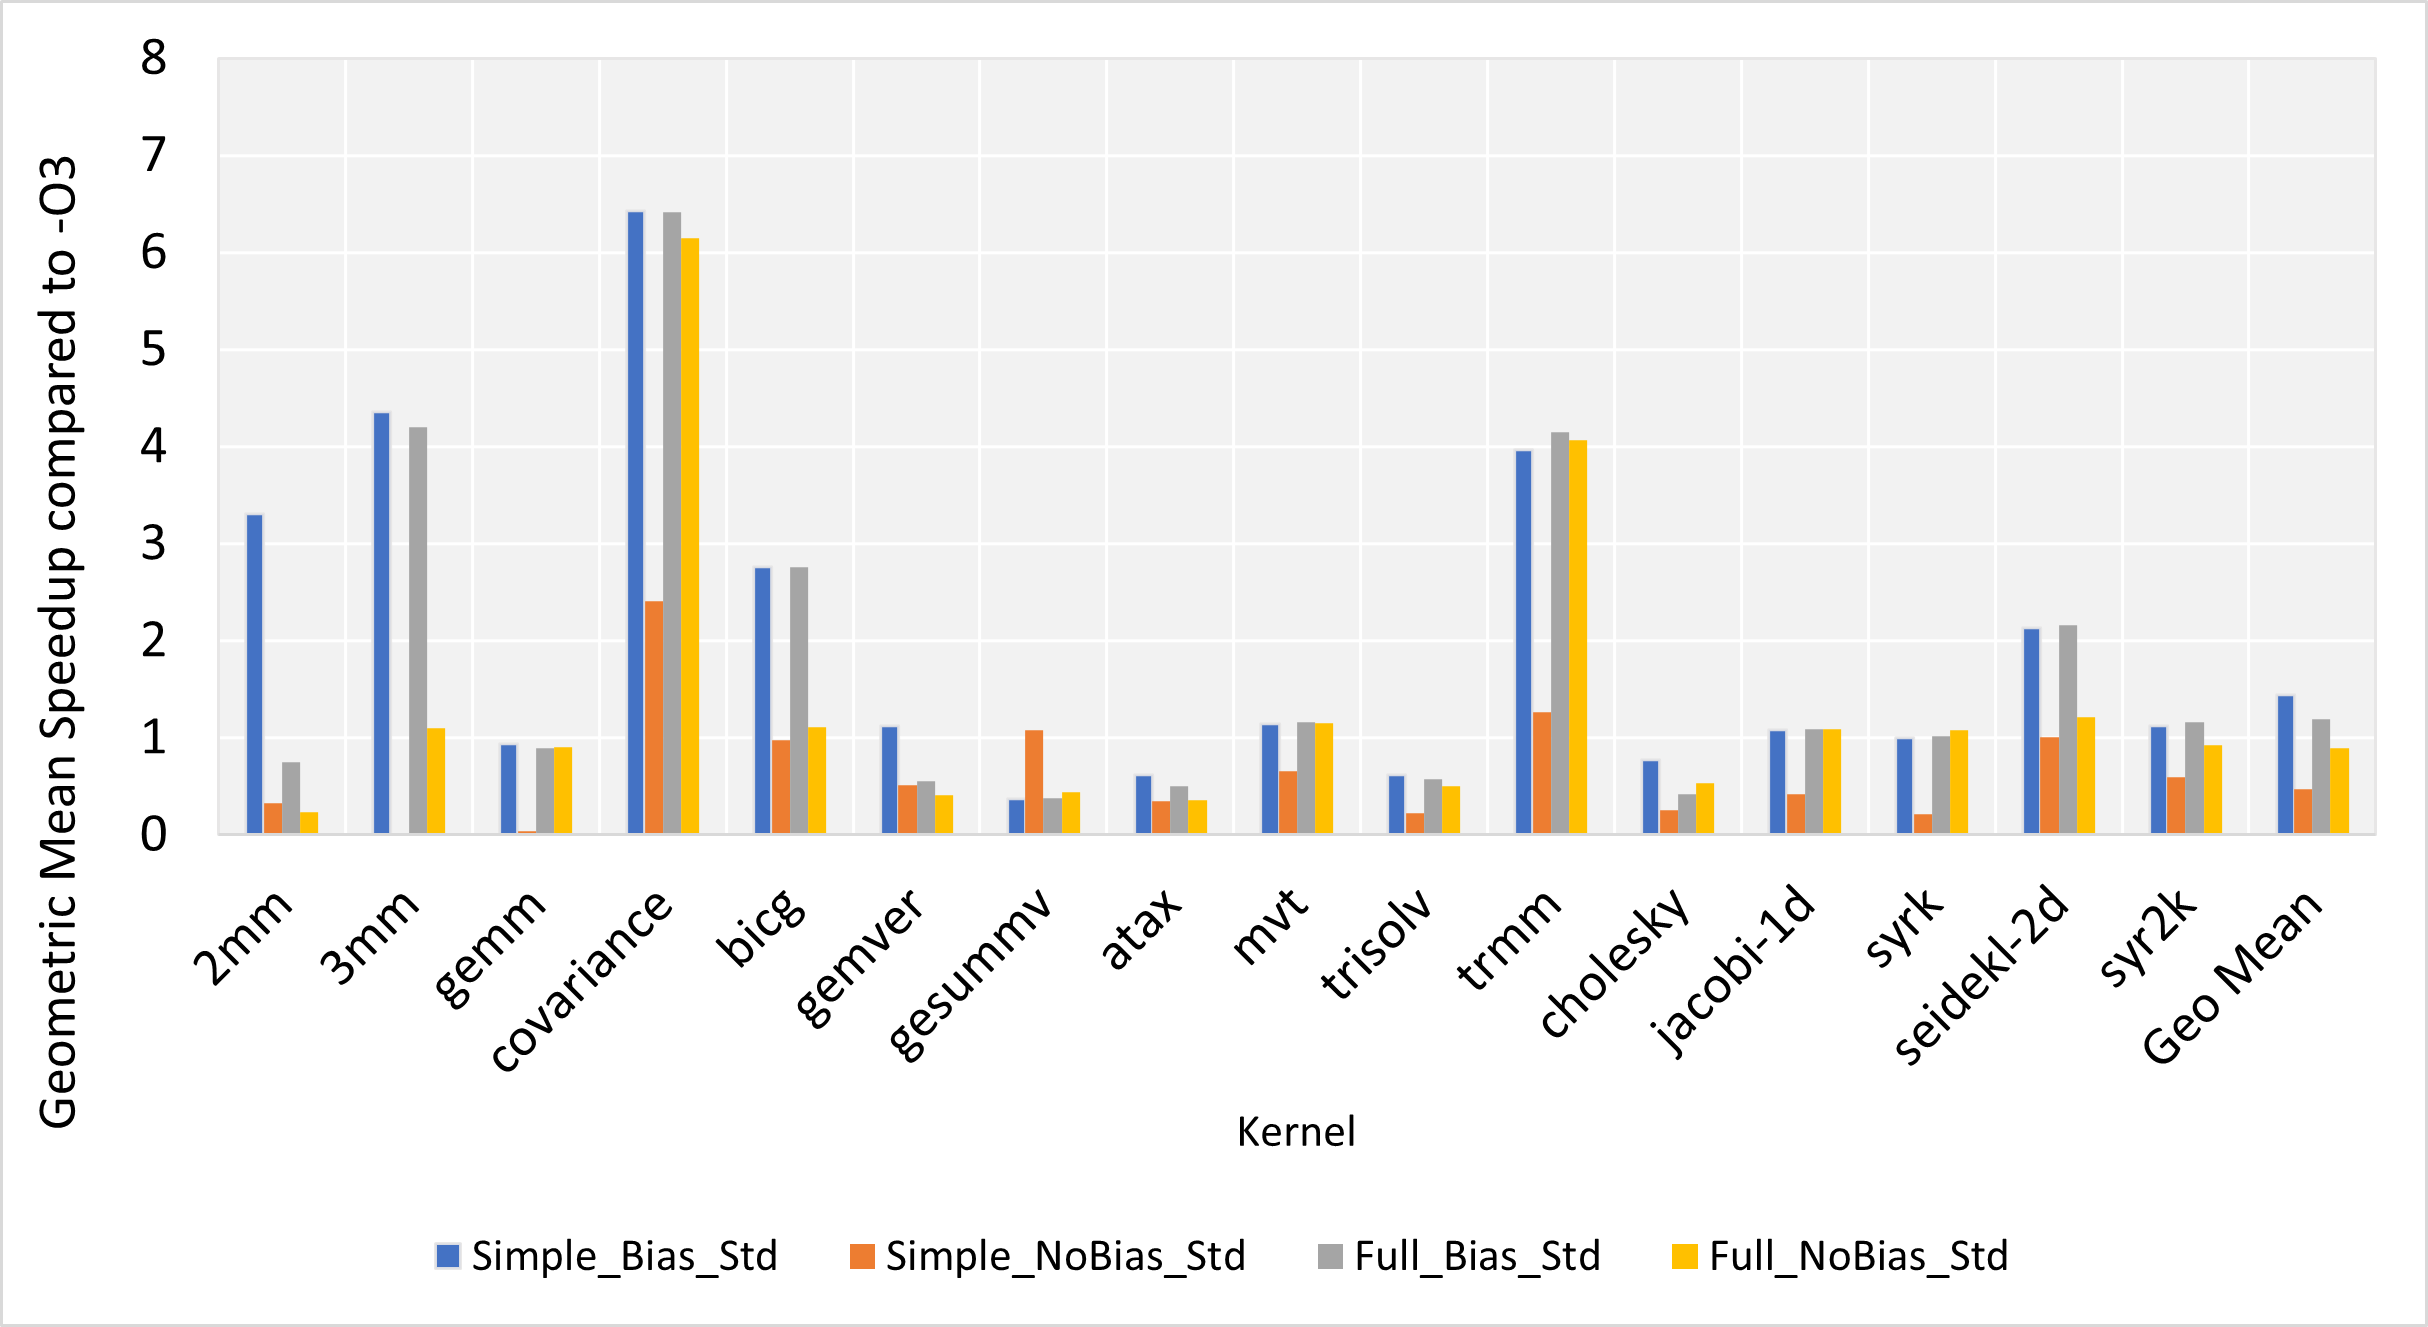
\includegraphics[width=\linewidth]{Images/Std_Chart.png}
  \captionof{figure}{With Standardisation (Mean: 1.40)}
  \label{fig:Std_Chart}
\end{minipage}
\hspace{.05\linewidth}
\begin{minipage}{.45\linewidth}
  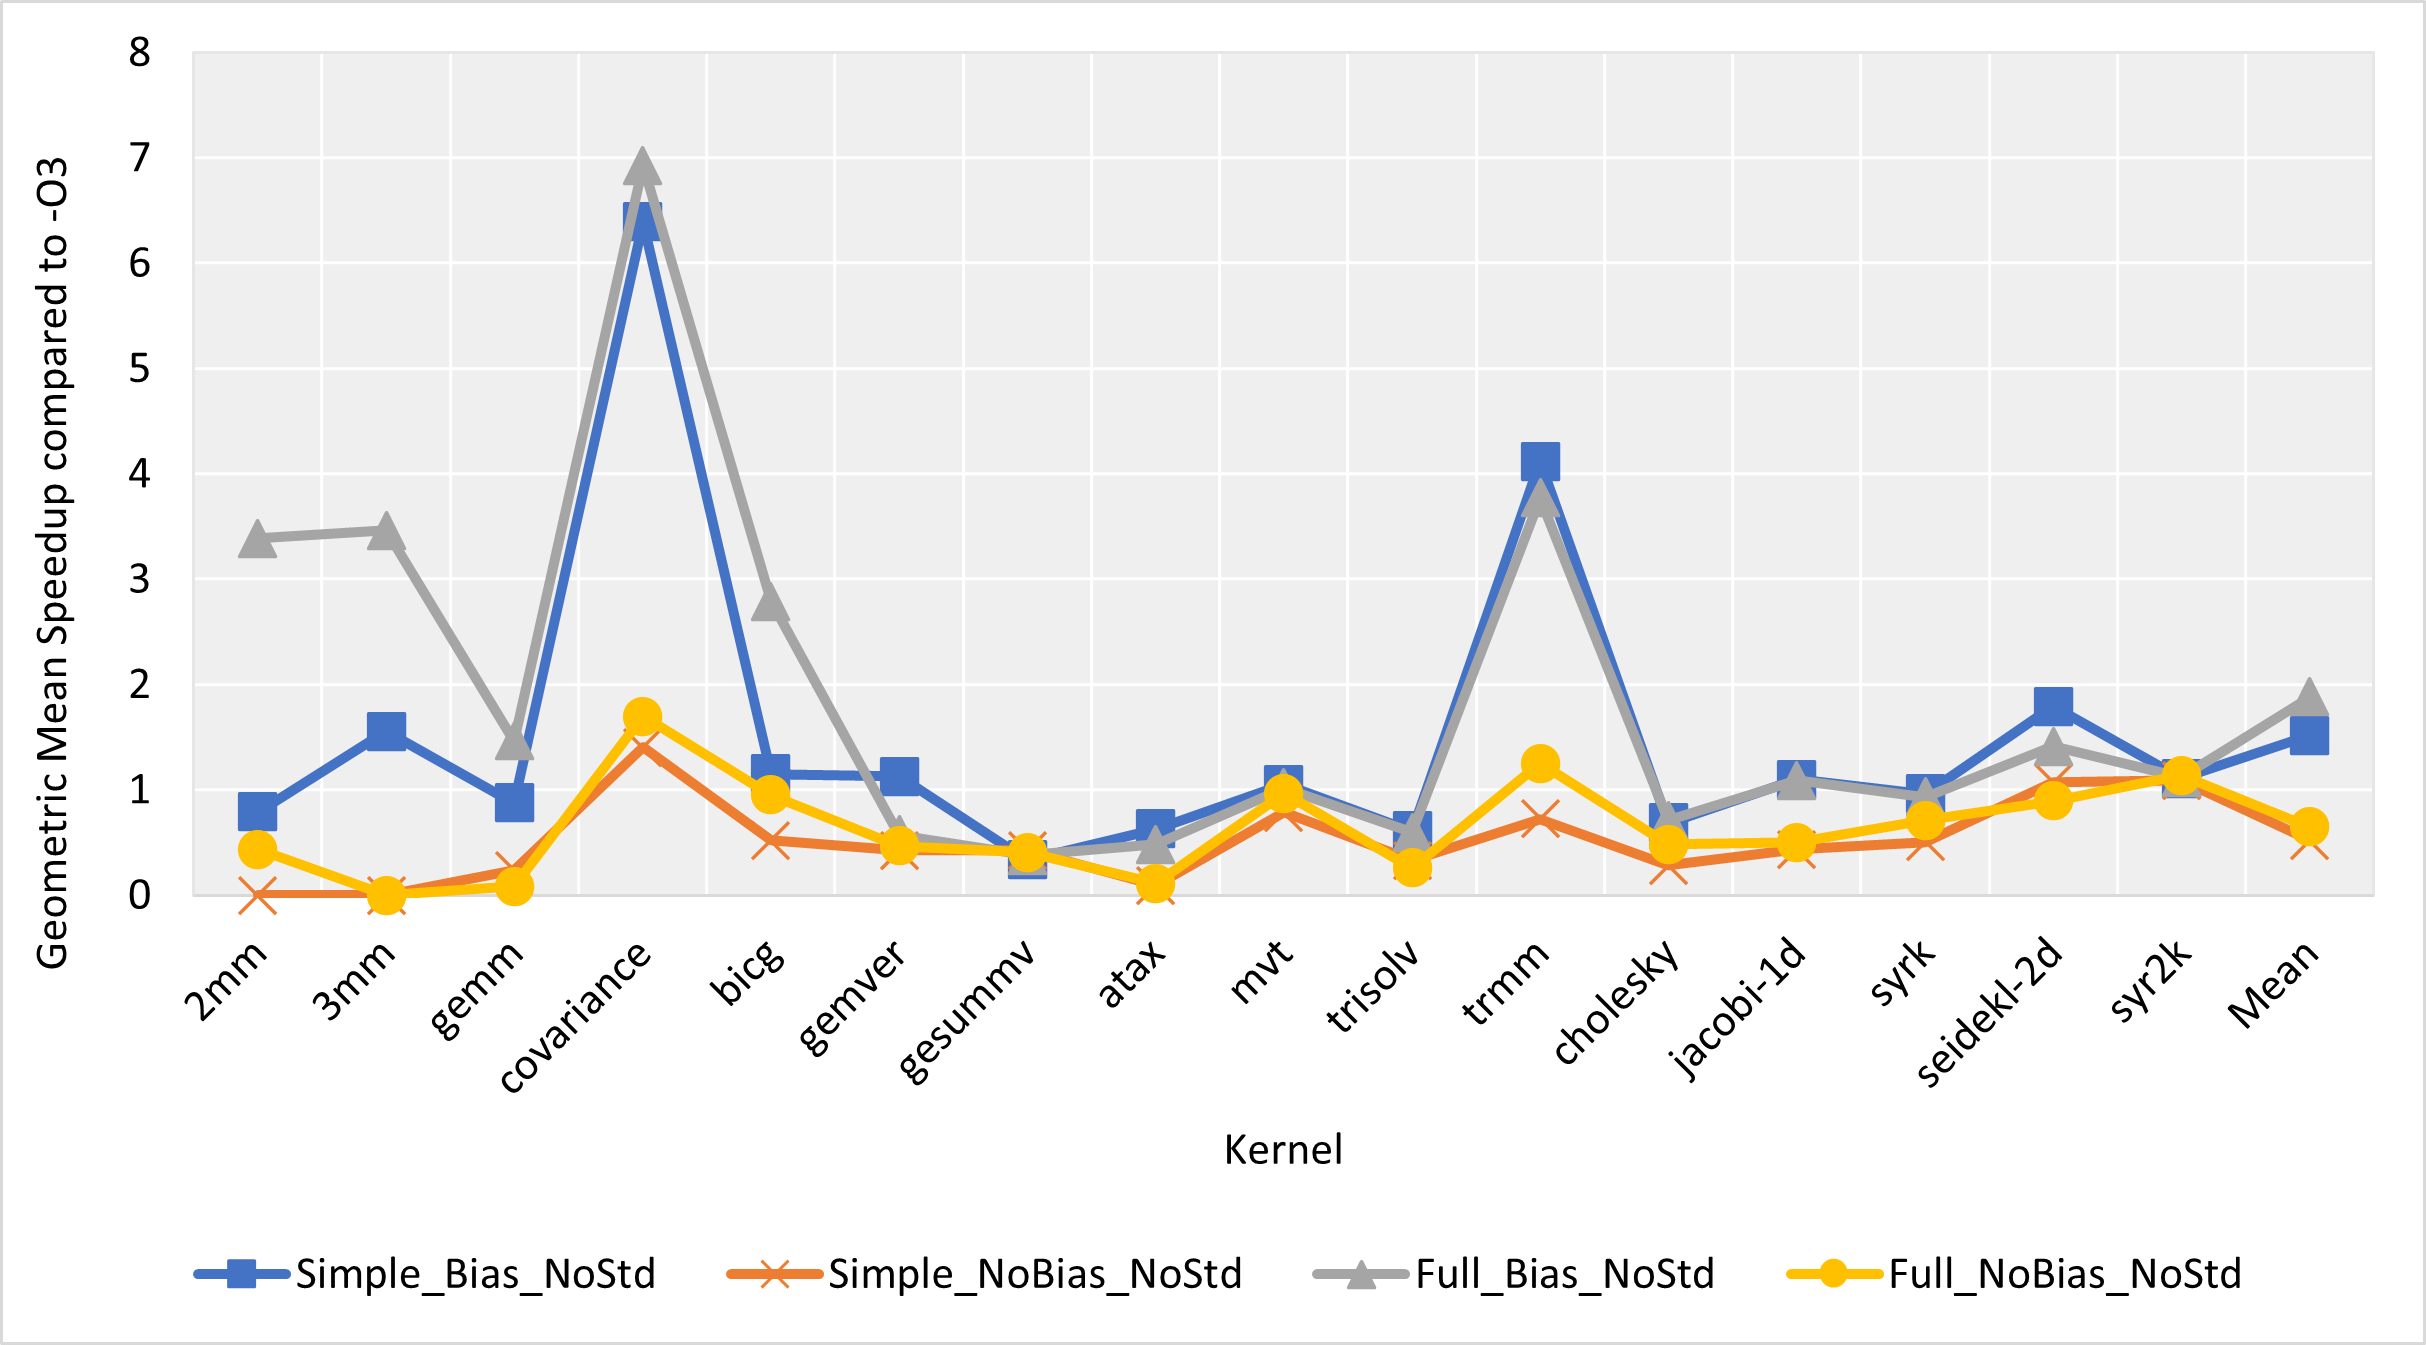
\includegraphics[width=\linewidth]{Images/NoStd_Chart.png}
  \captionof{figure}{Without Standardisation (Mean: 1.14)}
  \label{fig:NoStd_Chart}
\end{minipage}
\State{Comparison of PolyGymRL Results for Standardisation and No Standardisation Approach}
\end{figure}

\begin{figure}
\centering
\begin{minipage}{.45\linewidth}
  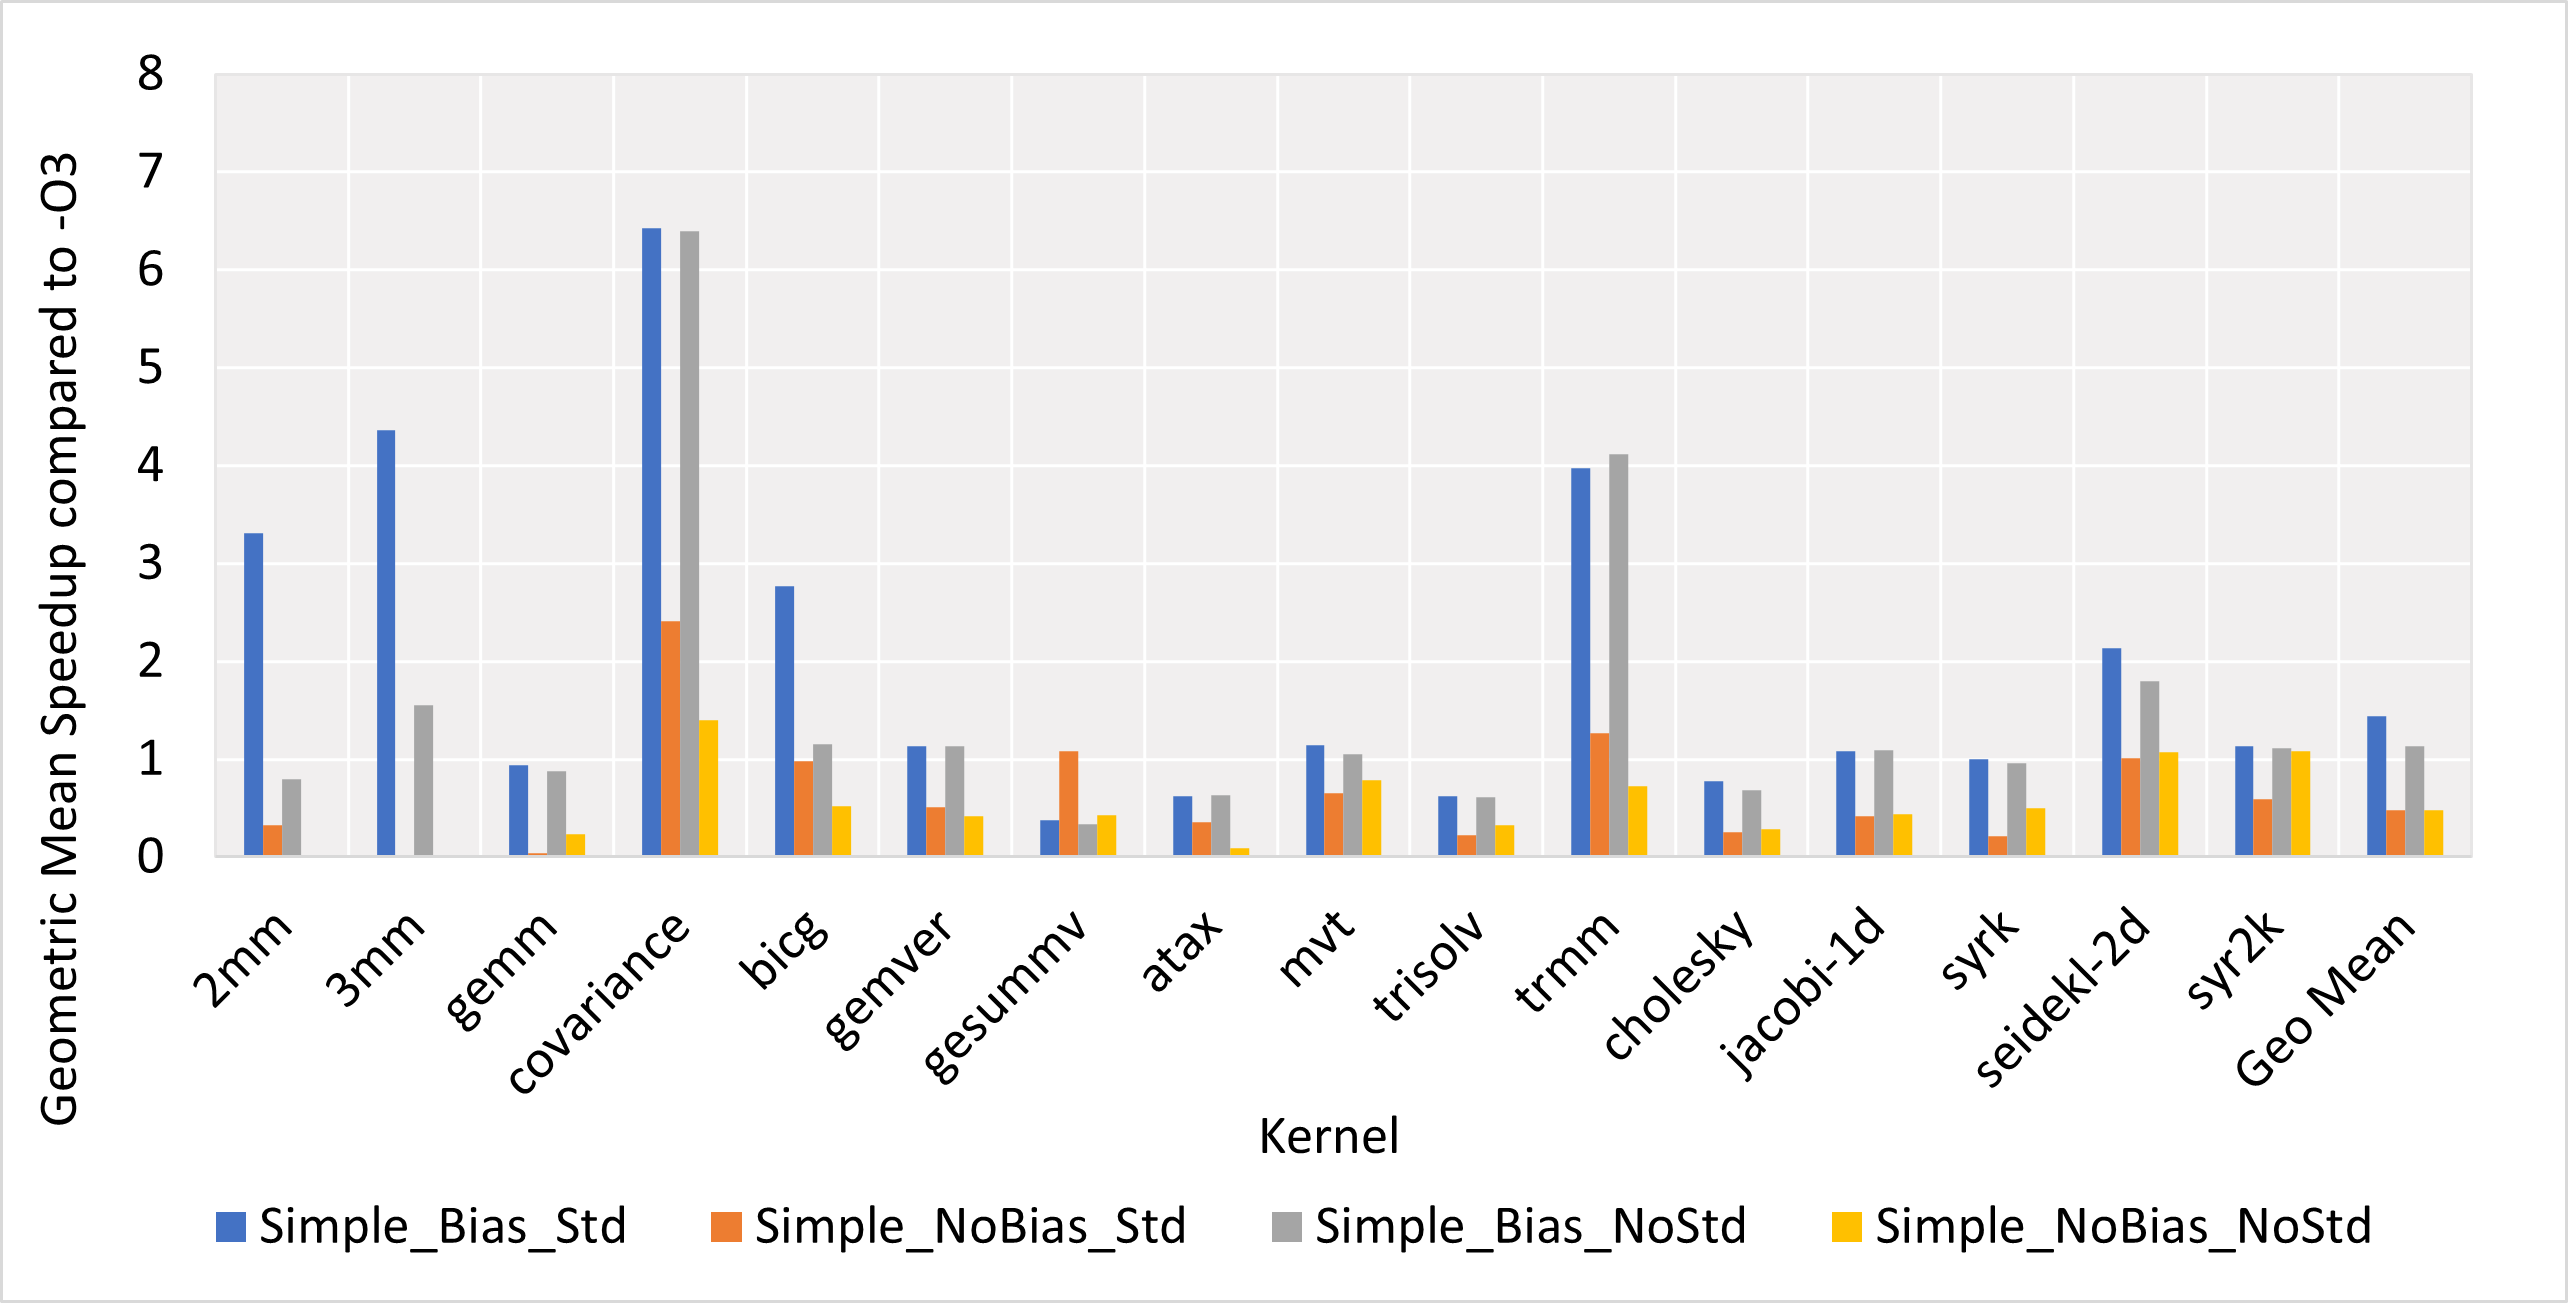
\includegraphics[width=\linewidth]{Images/Simple_Chart.png}
  \captionof{figure}{Simple Representation (Mean: 0.98)}
  \label{fig:Simple_Chart}
\end{minipage}
\hspace{.05\linewidth}
\begin{minipage}{.45\linewidth}
  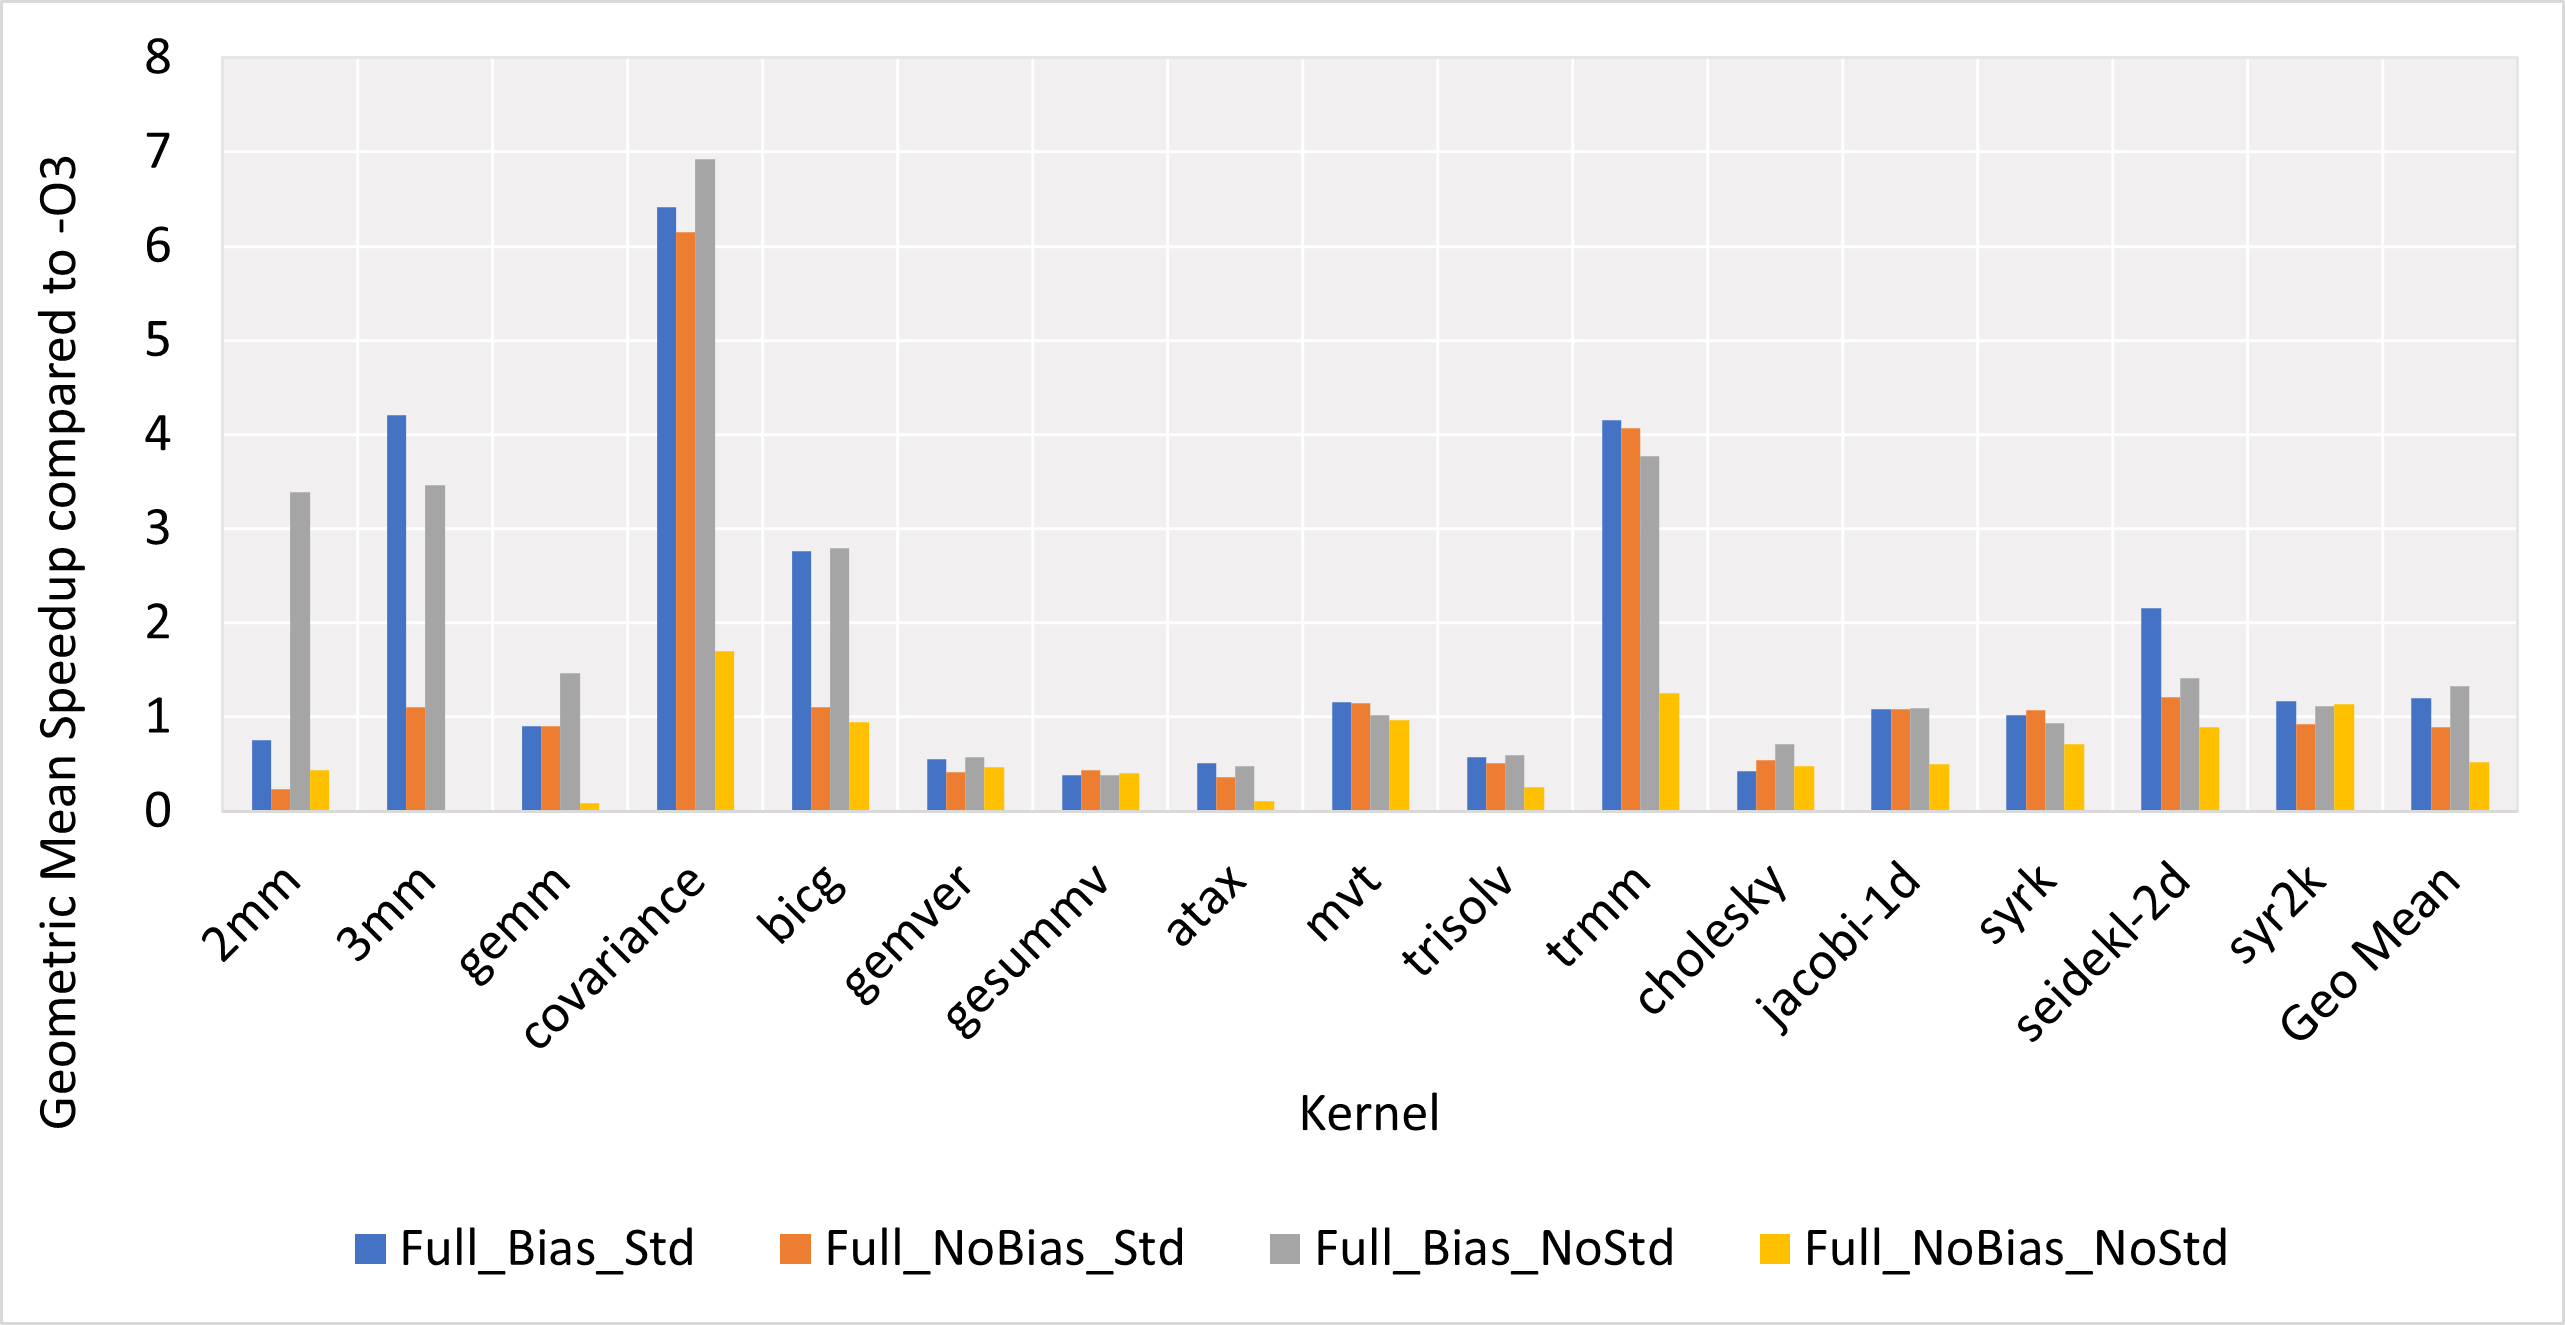
\includegraphics[width=\linewidth]{Images/NoSimple_Chart.png}
  \captionof{figure}{Full Representation (Mean: 1.40)}
  \label{fig:NoSimple_Chart}
\end{minipage}
\State{Comparison of PolyGymRL Results for Simple and Full Representation}
\end{figure}

\begin{figure}`
\centering
\begin{minipage}{.45\linewidth}
  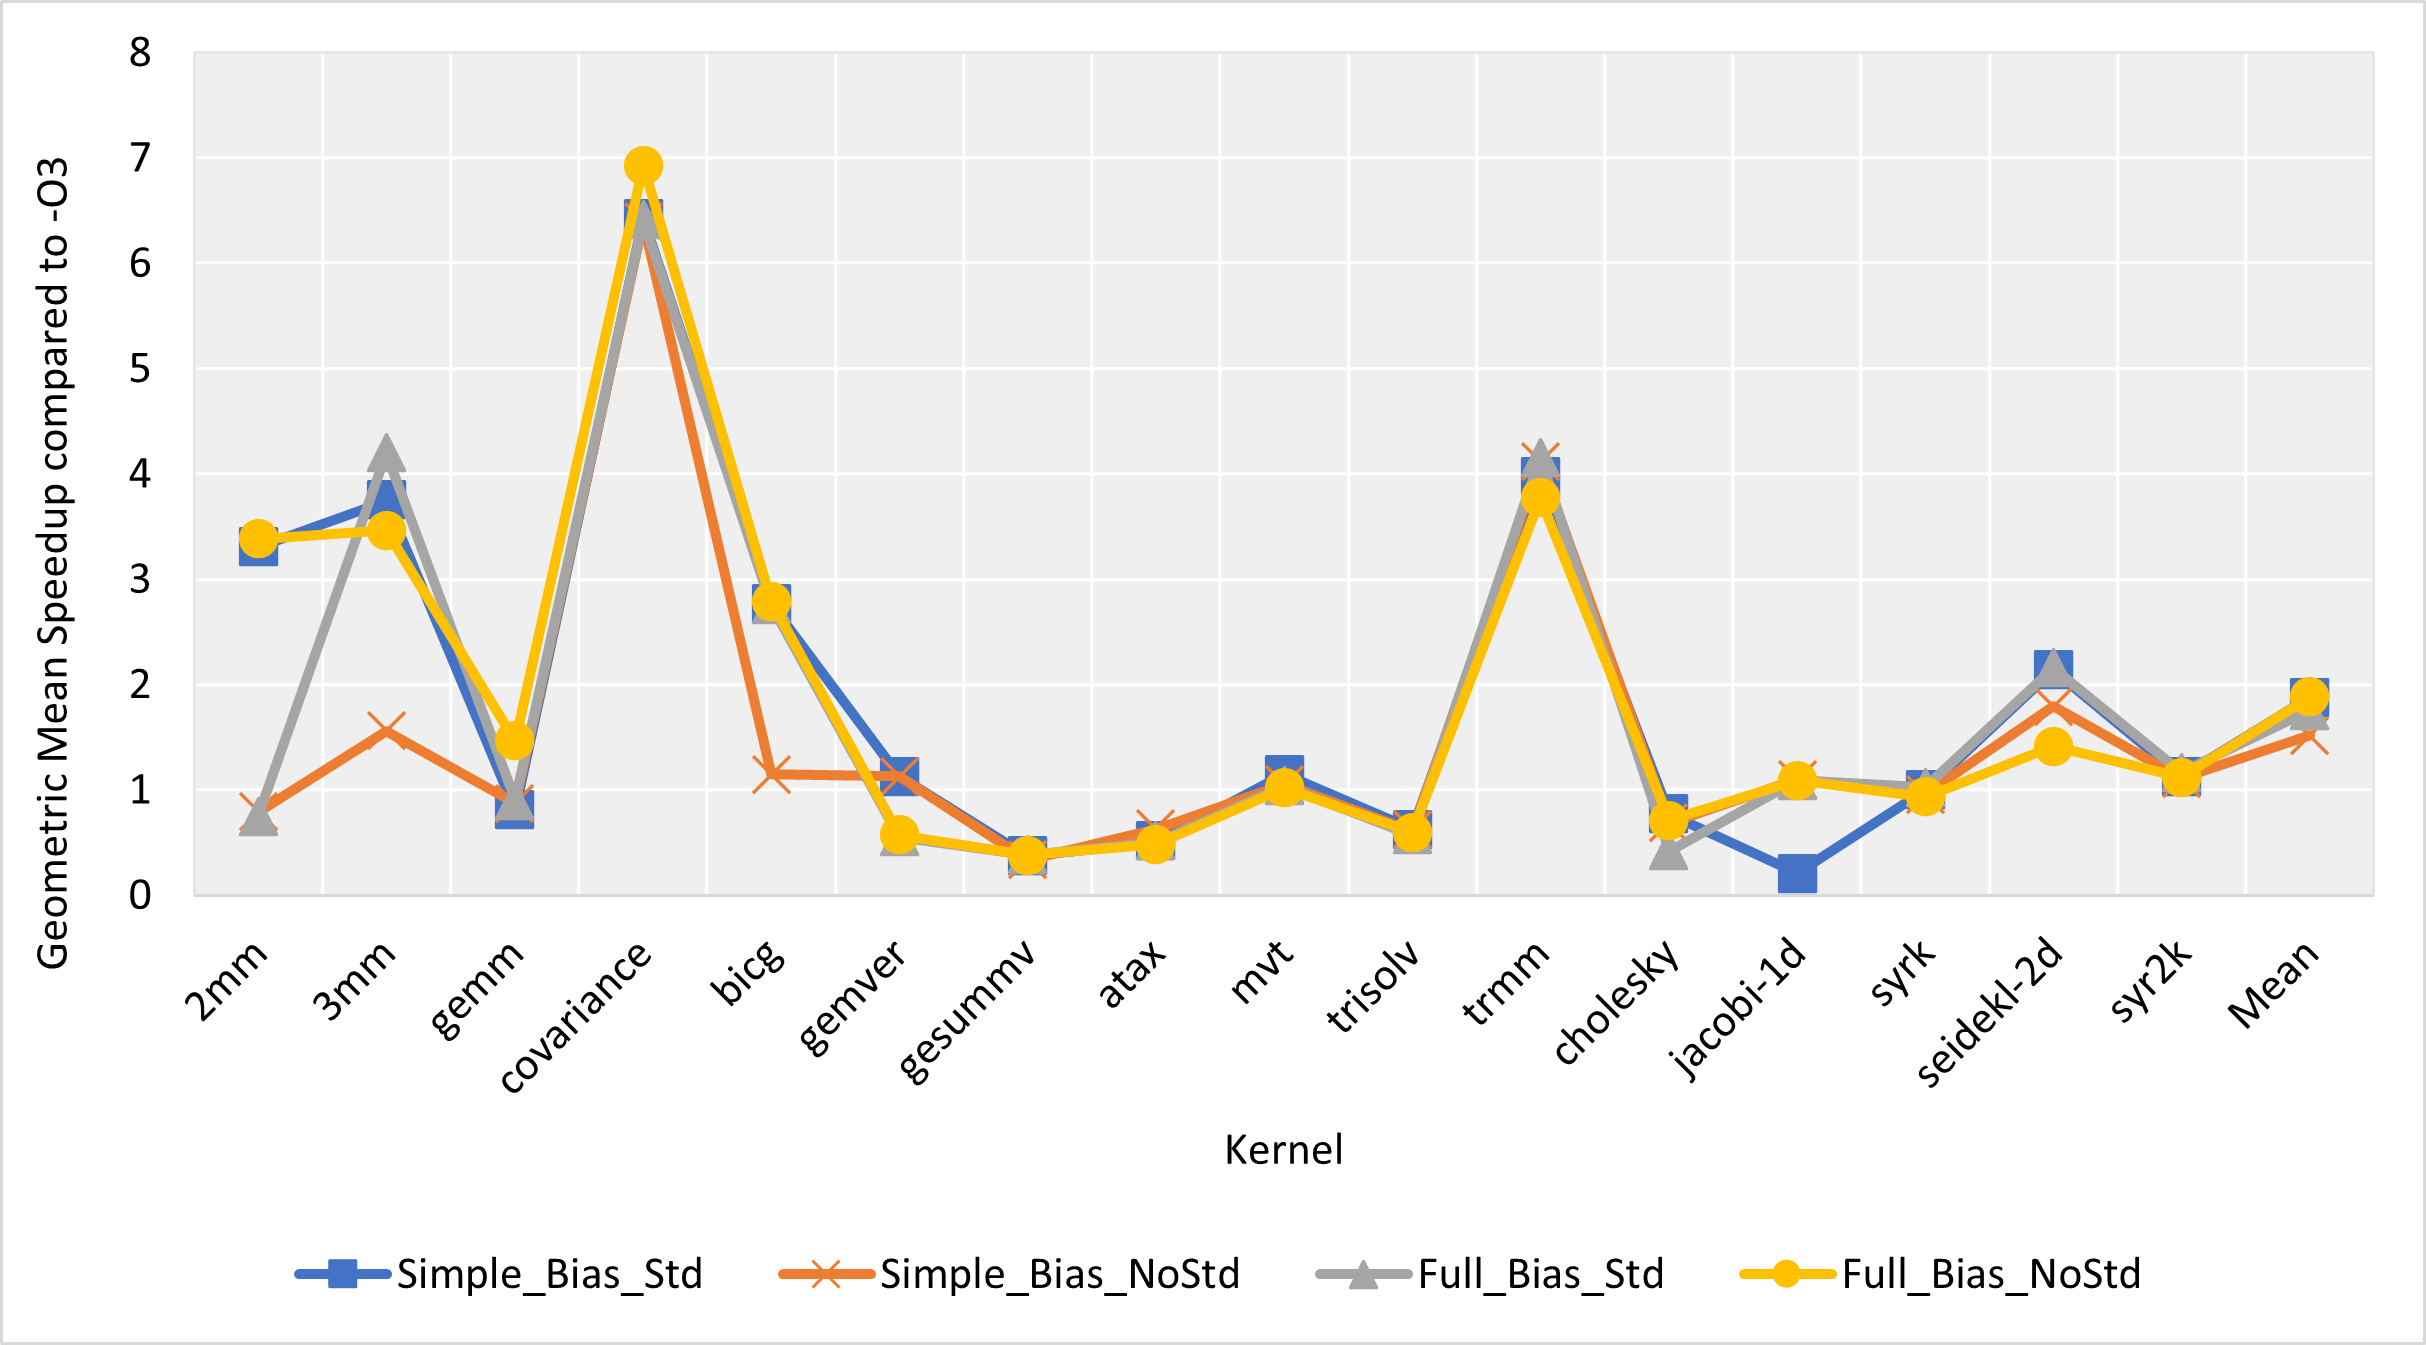
\includegraphics[width=\linewidth]{Images/Bias_Chart.png}
  \captionof{figure}{With Bias(Mean: 1.76)}
  \label{fig:Bias_Chart}
\end{minipage}
\hspace{.05\linewidth}
\begin{minipage}{.45\linewidth}
  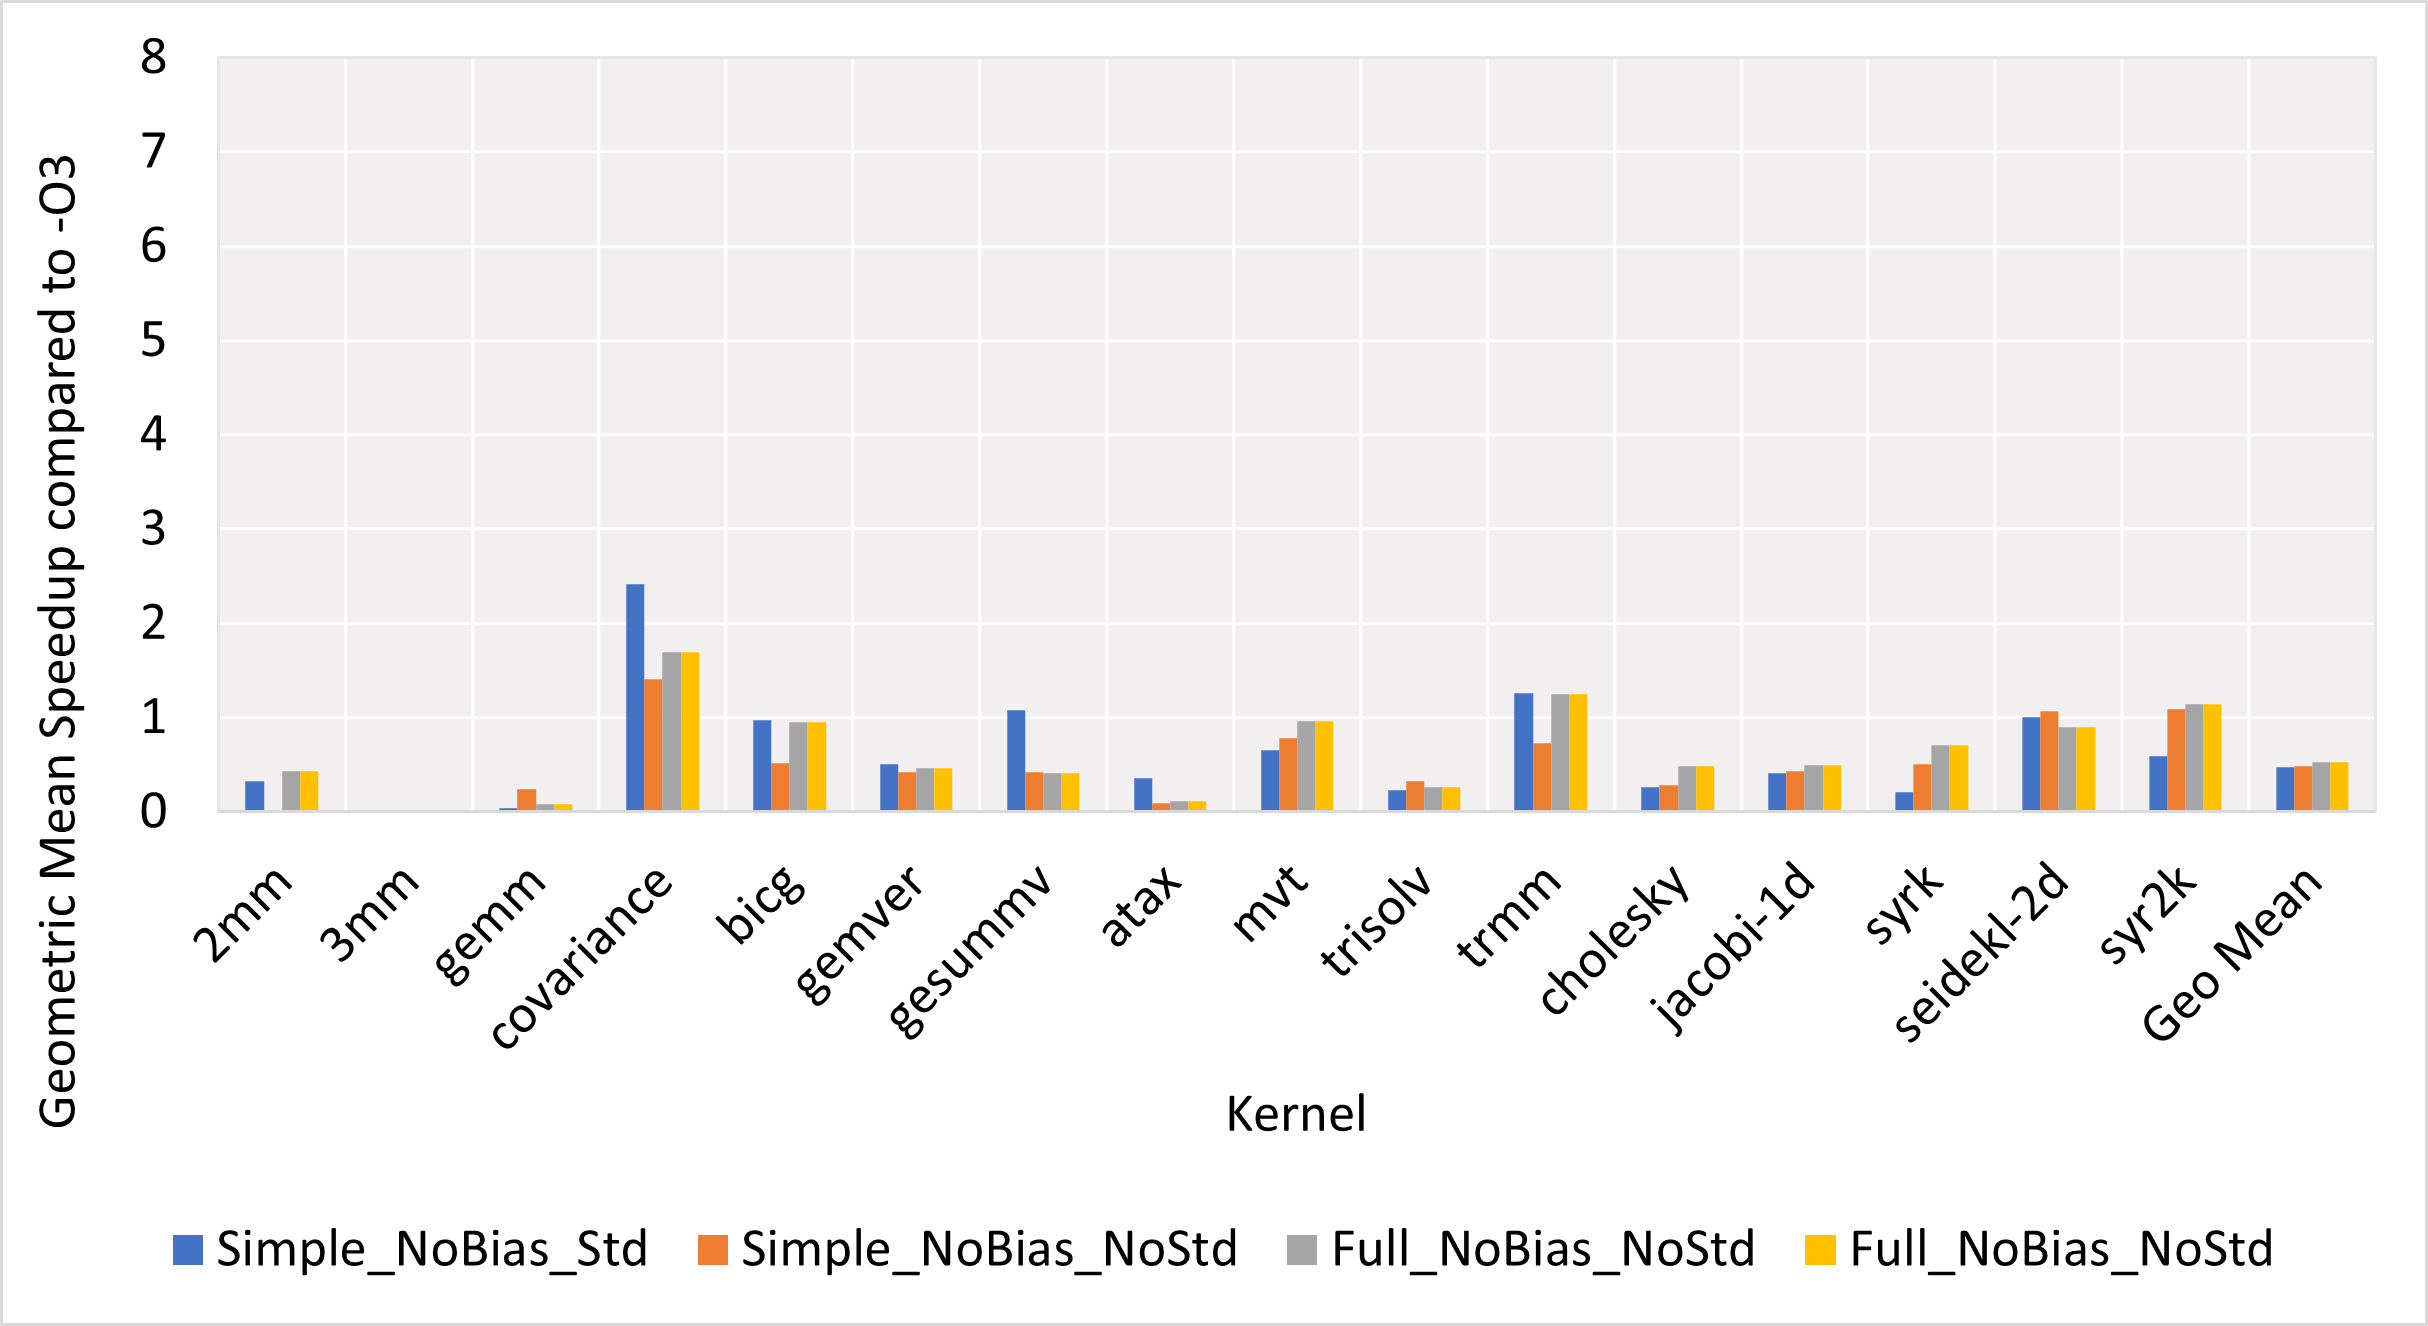
\includegraphics[width=\linewidth]{Images/NoBias_Chart.png}
  \captionof{figure}{Without Bias(Mean: 0.79)}
  \label{fig:NoBias_Chart}
\end{minipage}
\State{Comparison of PolyGymRL Results with and without bias while selecting coefficients}
\end{figure}

\begin{figure}
\centering
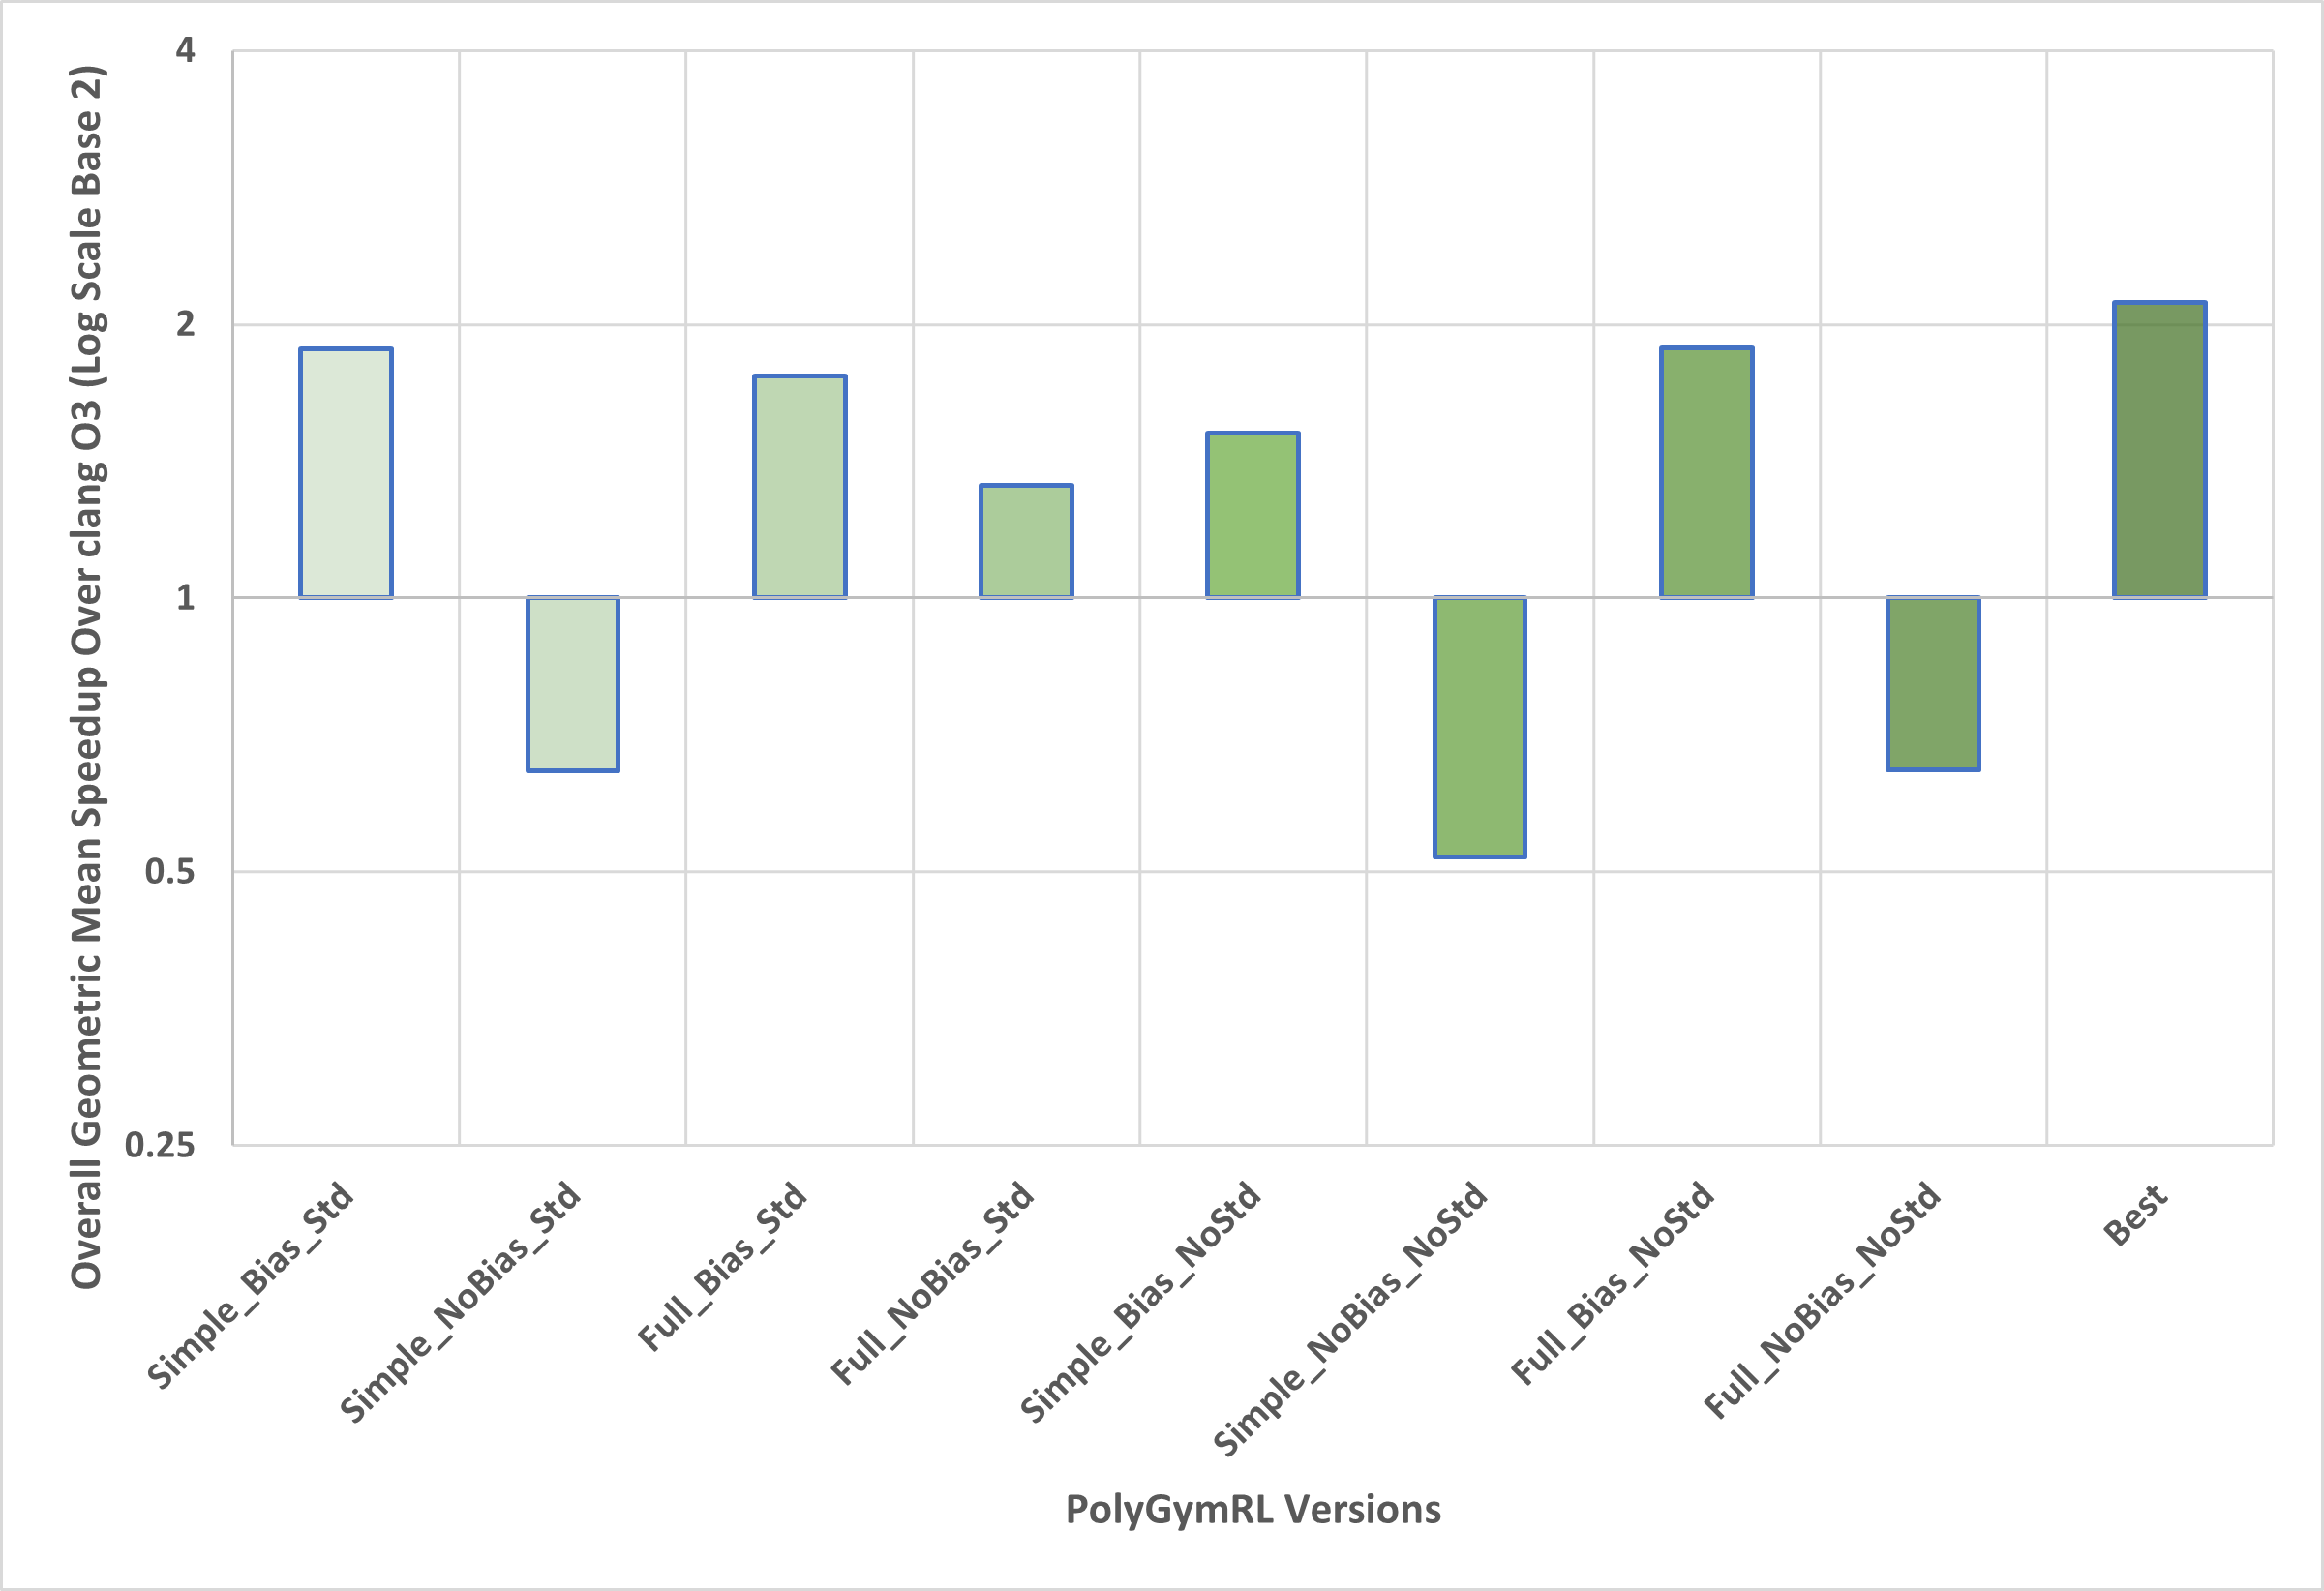
\includegraphics[width=\linewidth]{Images/PolyGymRL_Versions.png}
\captionof{figure}{Comparison of Speedup for different PolyGymRL Versions}
\label{fig:PolyGymRL_Versions}
\end{figure}

\begin{figure}
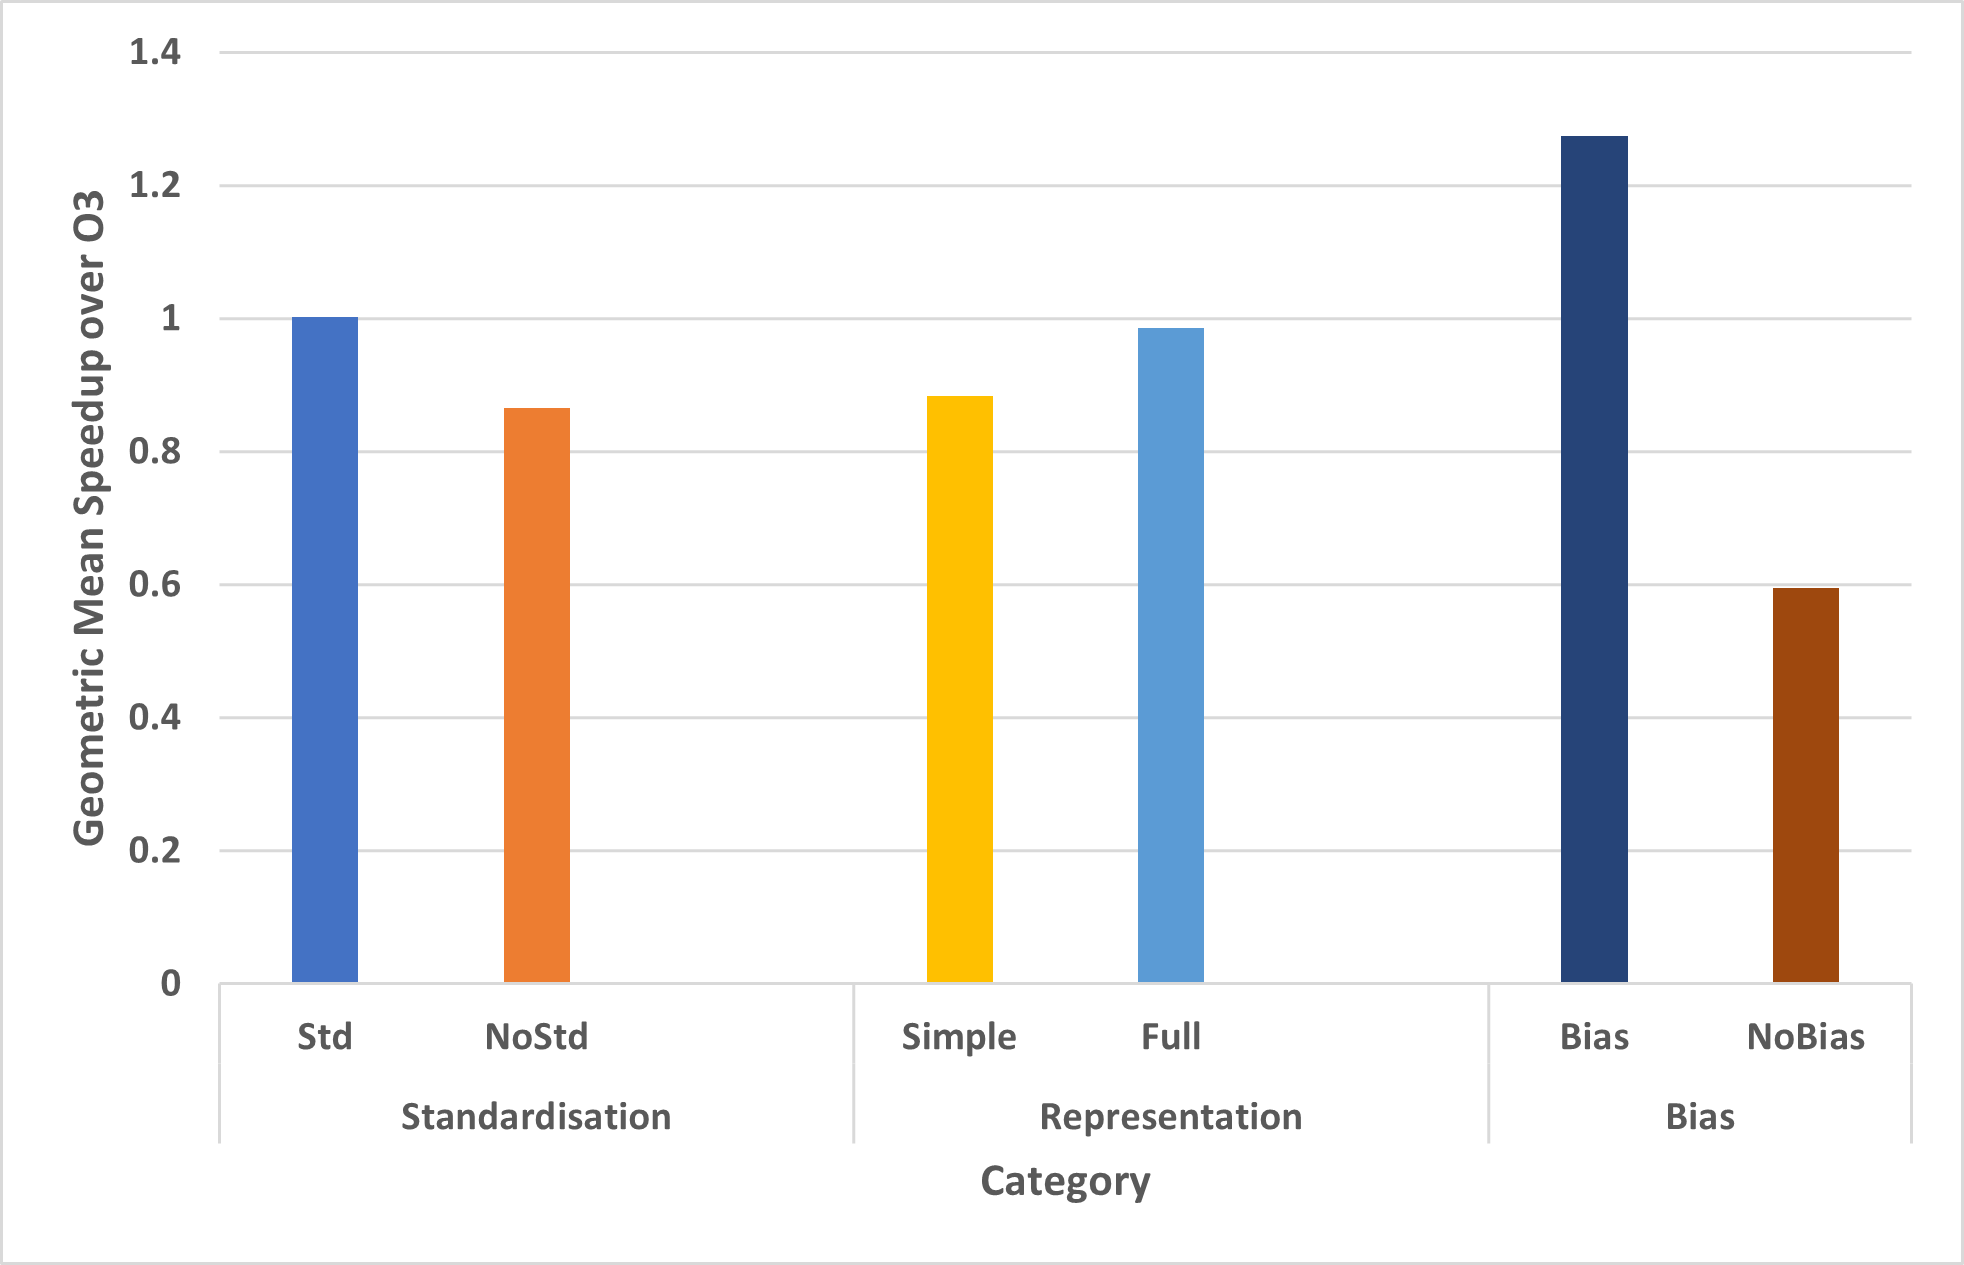
\includegraphics[width=\linewidth]{Images/PolyGymRL_Strategies.png}
\captionof{figure}{Comparison of Speedup for different PolyGymRL Strategies}
\label{fig:PolyGymRL_Strategies}
\end{figure}

Figure \ref{fig:PolyGymRL_Strategies} shows category wise comparison of different approaches undertaken in the study. What is interesting about the data in this table is that it clearly demonstrates that better schedules can be generated while applying standardisation, using full representation and keeping the bias toward selecting coefficients. Interestingly though, the version involving bias, full representation and standardisation does not yield the best result among all. This is a rather unexpected outcome. Surprisingly, some kernels like \textit{2mm} did not perform as well as expected under this category. In the below sections, we have discussed possible reasons for some inconsistencies in the findings and not very significant performances of some kernels. More advanced algorithms and effective parameter search, such as the number of schedules, training iterations, and learning parameters which were not the point of focus in this study, may help resolve some of the issues and improve what we have implemented until now.

\section{Limitation of the Training Set}
The training set we have selected is limited and it is unlikely that it might represent all the required characteristics for generating a performant schedule. The construction phase state representation has nearly 300 variables, and the explorations state has more than 1000 variables. For the construction phase, if we assume that each of the 300 variables has a range of 3 different values (although some features like dimensions are not bounded and can have more than 10 values), there are 45451 combinations possible just for the construction. For exploration, it can easily exceed 500 thousand combination possibilities. While this is not a bottleneck in terms of computation anymore, it is vital to have enough data to make learning accurate. No matter how clever the algorithm is, it may not beat a simple algorithm with extensive data, as the underlying approximation will mostly stay the same with different algorithms. The number of dependencies varies from 2 to 81 in the subset of just more than 15 kernels we have chosen. Hence, while testing a new kernel, we may not encounter any "nearby" cases from the training. This is just one of many factors associated with the limitations of our results in this experiment. 

\section{Varying State Sizes in Reinforcement Learning}
As stated earlier, another issue related to the type of problem in the discussion is that the state size varies significantly with each kernel. For a simple kernel like \textit{mvt}, the number of dimensions is 1, and the list of generators has a size of 8 during the exploration phase. While in the case of \textit{3mm}, the dimension size is 7, each containing 51 vertices and rays. Thus, the difference in the size of the state is vast. This difference makes the implementation of Reinforcement Learning algorithms on this problem a complex task, especially for those involving either some form of approximation or deep learning. One has to consider the right choice of representation for the features and other typical values of the features. For the kernel requiring a smaller state size, a more extensive state size might add some noise to the learning procedure, increasing the number of computations and memory required to store the data.

\section{The Necessity and Effects of Standardisation}
\label{sec:std}
The range of values of different features used in the representation varies considerably in this experiment. The number of dimensions theoretically varies in the range of (0, $\infty$). The dependency representation in the form of linear inequalities gives values in the range of (-$\infty$, $\infty$). The dependencies added in the current dimensions are either 0 or 1. At the same time, the points resulting from the coefficients and the generators in each dimension ranges from (-$\infty$, $\infty$) during exploration. Thus, various state features are unbounded, for example, the number of dimensions in the construction phase, or the number and length of the generators in the exploration phase. Without standardisation, the weights of the Q-learning can quickly go to infinity. Moreover, the importance of all the features remains inconsistent leading to incorrect learning. On the other hand, standardising the values is only straightforward with the apparent minimum and maximum values. To convert the values ranging from (-$\infty$, $\infty$) to (0,1), we have used the standard logistic function \[{1/1+e^{-x}}\]. While to convert (0, $\infty$) to (0,1), we have used the function \[{x / (1 + x)}\]. This standardisation helps keep the weights within the limit and gives equal importance to all the features. However, there will always be some loss of information due to this.

\begin{figure}[htbp]
  \centering
  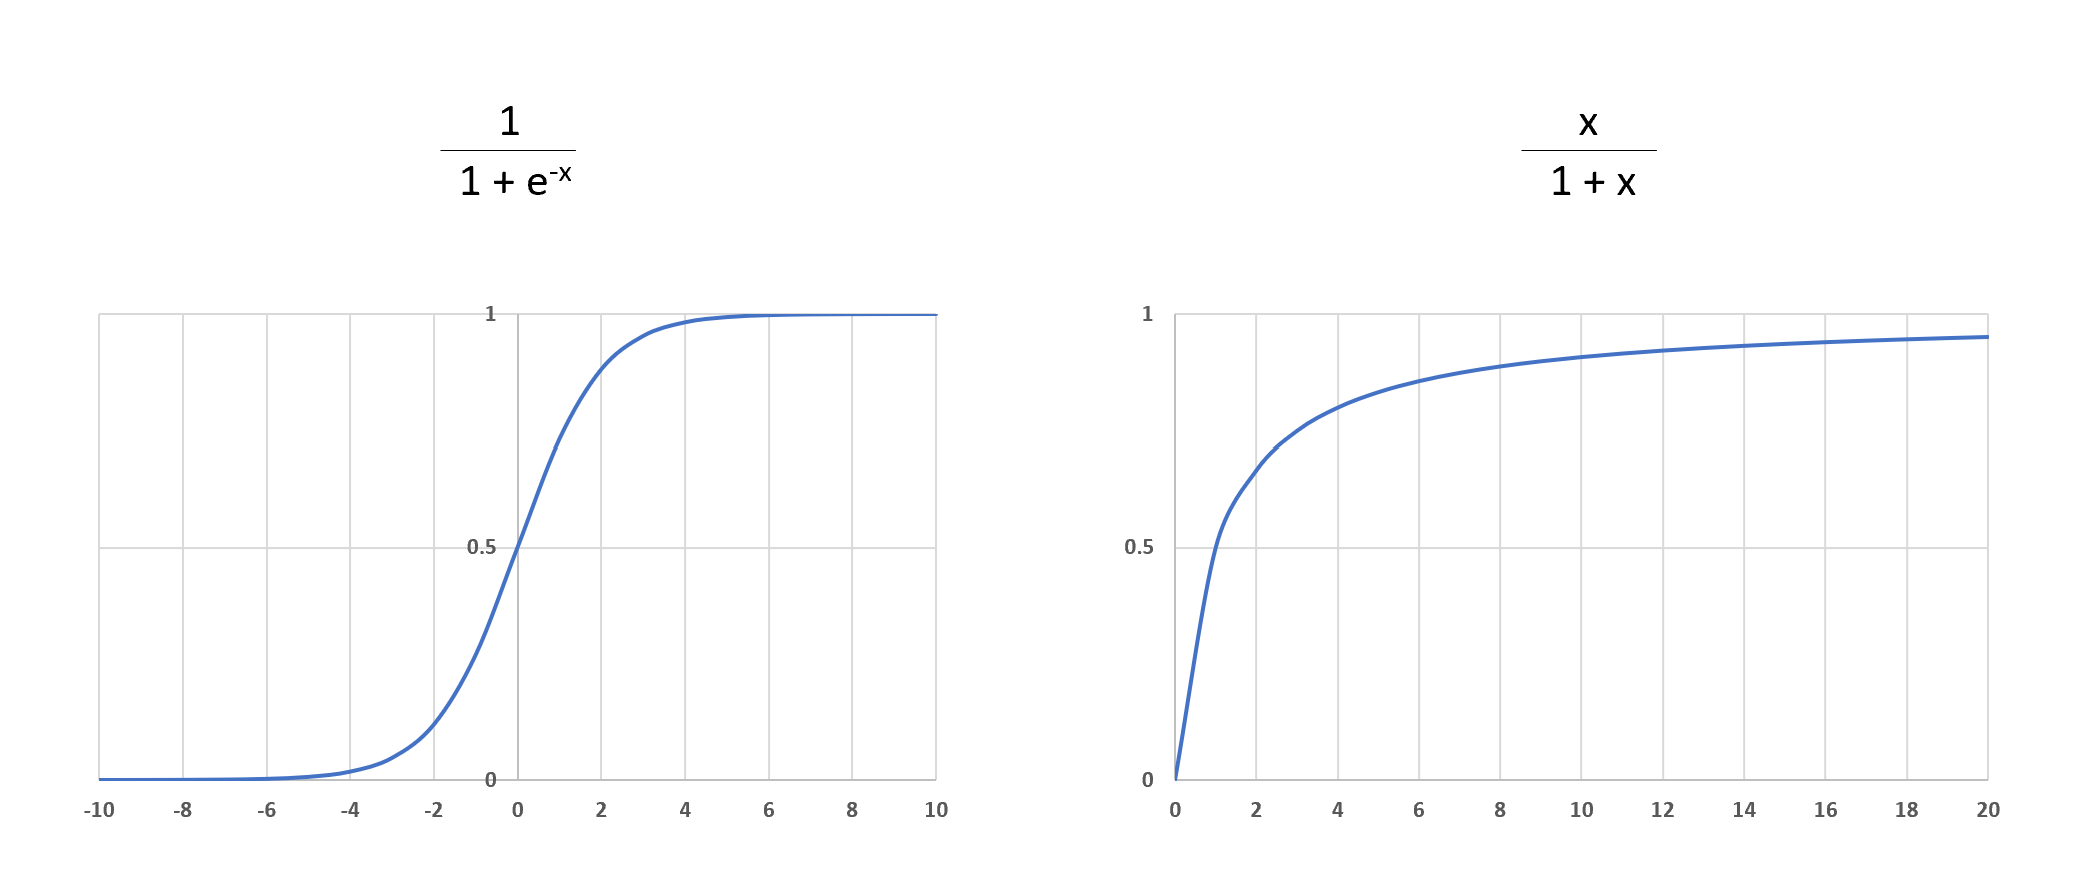
\includegraphics[width=\textwidth]{Images/Standardisation.png}    
  \caption{Standardisation Functions used in PolyGymRL Features}
  \label{fig:Standardisation}
\end{figure}


\chapter{Conclusions}

There were two most challenging aspects associated with the investigation in the discussion. Firstly, understanding polyhedral models presents a technical barrier that makes this type of research difficult. Secondly, even though we have taken just a subset of the kernels from all the possibilities in the industrial practice, it is still a complex task to generalise a learning behaviour that can apply to a specific type of loop with a regular structure. A few general challenges are associated with applying RL algorithms to compiler optimizations. The representation space is huge, and evaluating as we run the programs to obtain the rewards takes time. Dealing with these challenges, we successfully implemented RL agents to learn the general characteristics of building a good schedule irrespective of the test loop. At the same time, PolyGymRL presents an opportunity and example to continue this research direction to try out more advanced algorithms to improve the loop execution performance.

\section{Unresolved Issues and Future Work}

A few unresolved issues need to be addressed in the future. While a few loops like \textit{covariance} achieved a speedup close to 8, we did not witness similar results with all the loops. In fact, for a few loops like \textit{atax}, the speedup was relatively less compared to clang -O3 flag. Other advanced Reinforcement Learning algorithms, especially deep reinforcement learning algorithms such as DQN \cite{DBLP:journals/corr/MnihKSGAWR13}, Double Deep Q-Networks \cite{DDQN} and Deep Deterministic Policy Gradients (DDPG) \cite{BHATNAGAR20092471} can be implemented and tested by keeping this implementation as a reference. An extensive hyper parameters scan can be performed related to learning rate, gamma, epsilon and, size and type of the neural networks, output functions in the case of deep learning. PolyIte already uses Genetic Algorithm for random exploration. Although certain loops may not be as learnable as others, there will always be a difference in the speedup found on the new schedules for different kernels.
Similarly, in this problem, applying a combination of Reinforcement Learning algorithms and Genetic Algorithms\cite{GA} can be interesting. We have already tried a variety of state representations to facilitate training, and more experiments can be continued in this direction. The reward shaping is kept relatively simple by distributing the speedup to all the action-state pairs. There can be a separate investigation to analyse if agent learning can be aided by rewarding good intermediate situations instead of just the final outcome.

There were a few kernels like \textit{durbin}, which involve a very high search space construction time crossing the timeout barrier; hence we had to leave them out of our research. Recent advancements in high performance computing and performance programming can make this construction faster and improve scalability. There can be simple changes reducing the memory and storage requirements. For example, a single RL agent can carry out both construction and exploration activities instead of two. However, some limitations related to time taken are the characteristics of the polyhedral compilation itself and have little to do with our research. Currently, the study is limited to the kernels provided by PolyBench. In future, we are optimistic that this experiment can be carried out on other real-world kernel scenarios.



\bibliographystyle{plain}
\bibliography{MLPC}


% You may delete everything from \appendix up to \end{document} if you don't need it.
\appendix

\chapter{Results Data}

\section{PolyGymRL Results}

\begin{figure}[htbp]
  \centering
  \includegraphics[width=0.95\textwidth]{Images/BenchMarking.png}    
  \caption{Result Data for PolyGymRL}
  \label{fig:BenchMarking}
\end{figure}

\section{Comparison of PolyGym and PolyGymRL}

\begin{figure}
\centering
\begin{minipage}{.45\linewidth}
  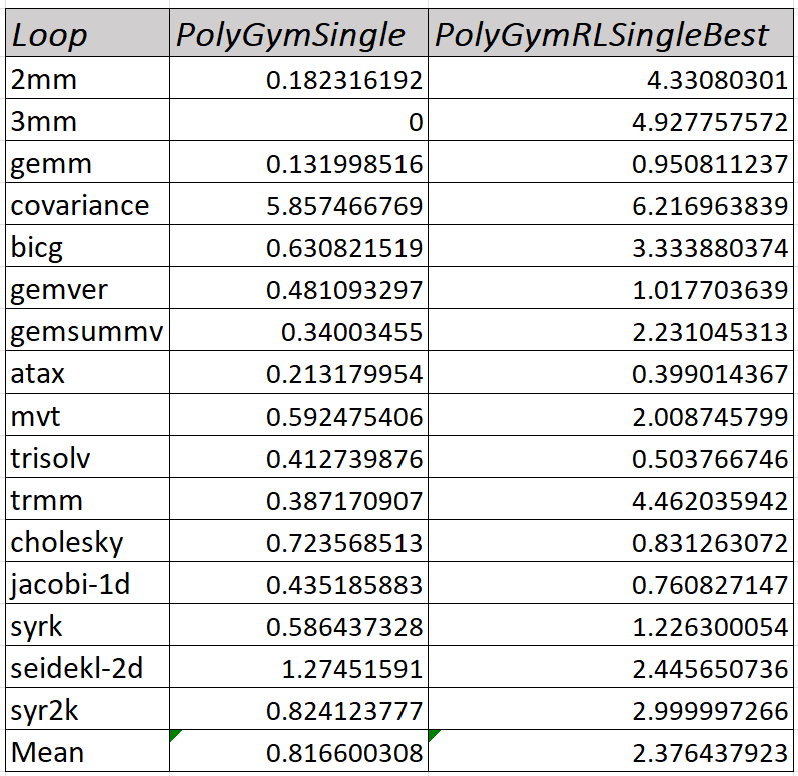
\includegraphics[width=\linewidth]{Images/Benchmarking_Single.png}
  \captionof{figure}{Results of PolyGym and PolyGymRL for single kernel}
  \label{Benchmarking_Single}
\end{minipage}
\hspace{.05\linewidth}
\begin{minipage}{.45\linewidth}
  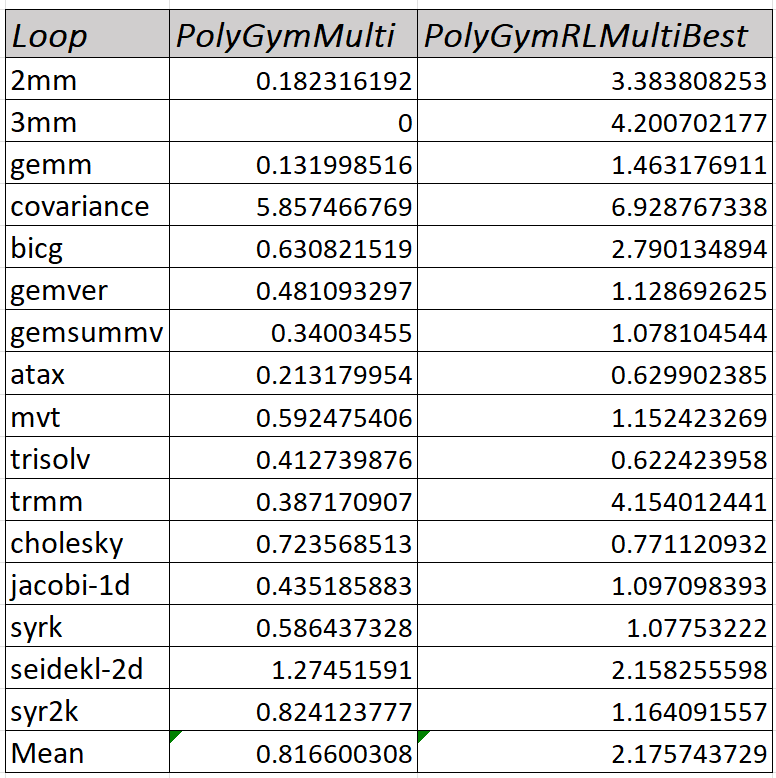
\includegraphics[width=\linewidth]{Images/Benchmarking_Multiple.png}
  \captionof{figure}{Results of PolyGym and PolyGymRL for multiple kernels}
  \label{Benchmarking_Multiple}
\end{minipage}
\State{Results Comparison of PolyGym and PolyGymRL for single and multiple kernels}
\end{figure}


\chapter{Results Graph}

\section{Comparison of PolyGymRL Versions}
\label{sec:Compare_Versions}

\begin{figure}[htbp]
  \centering
  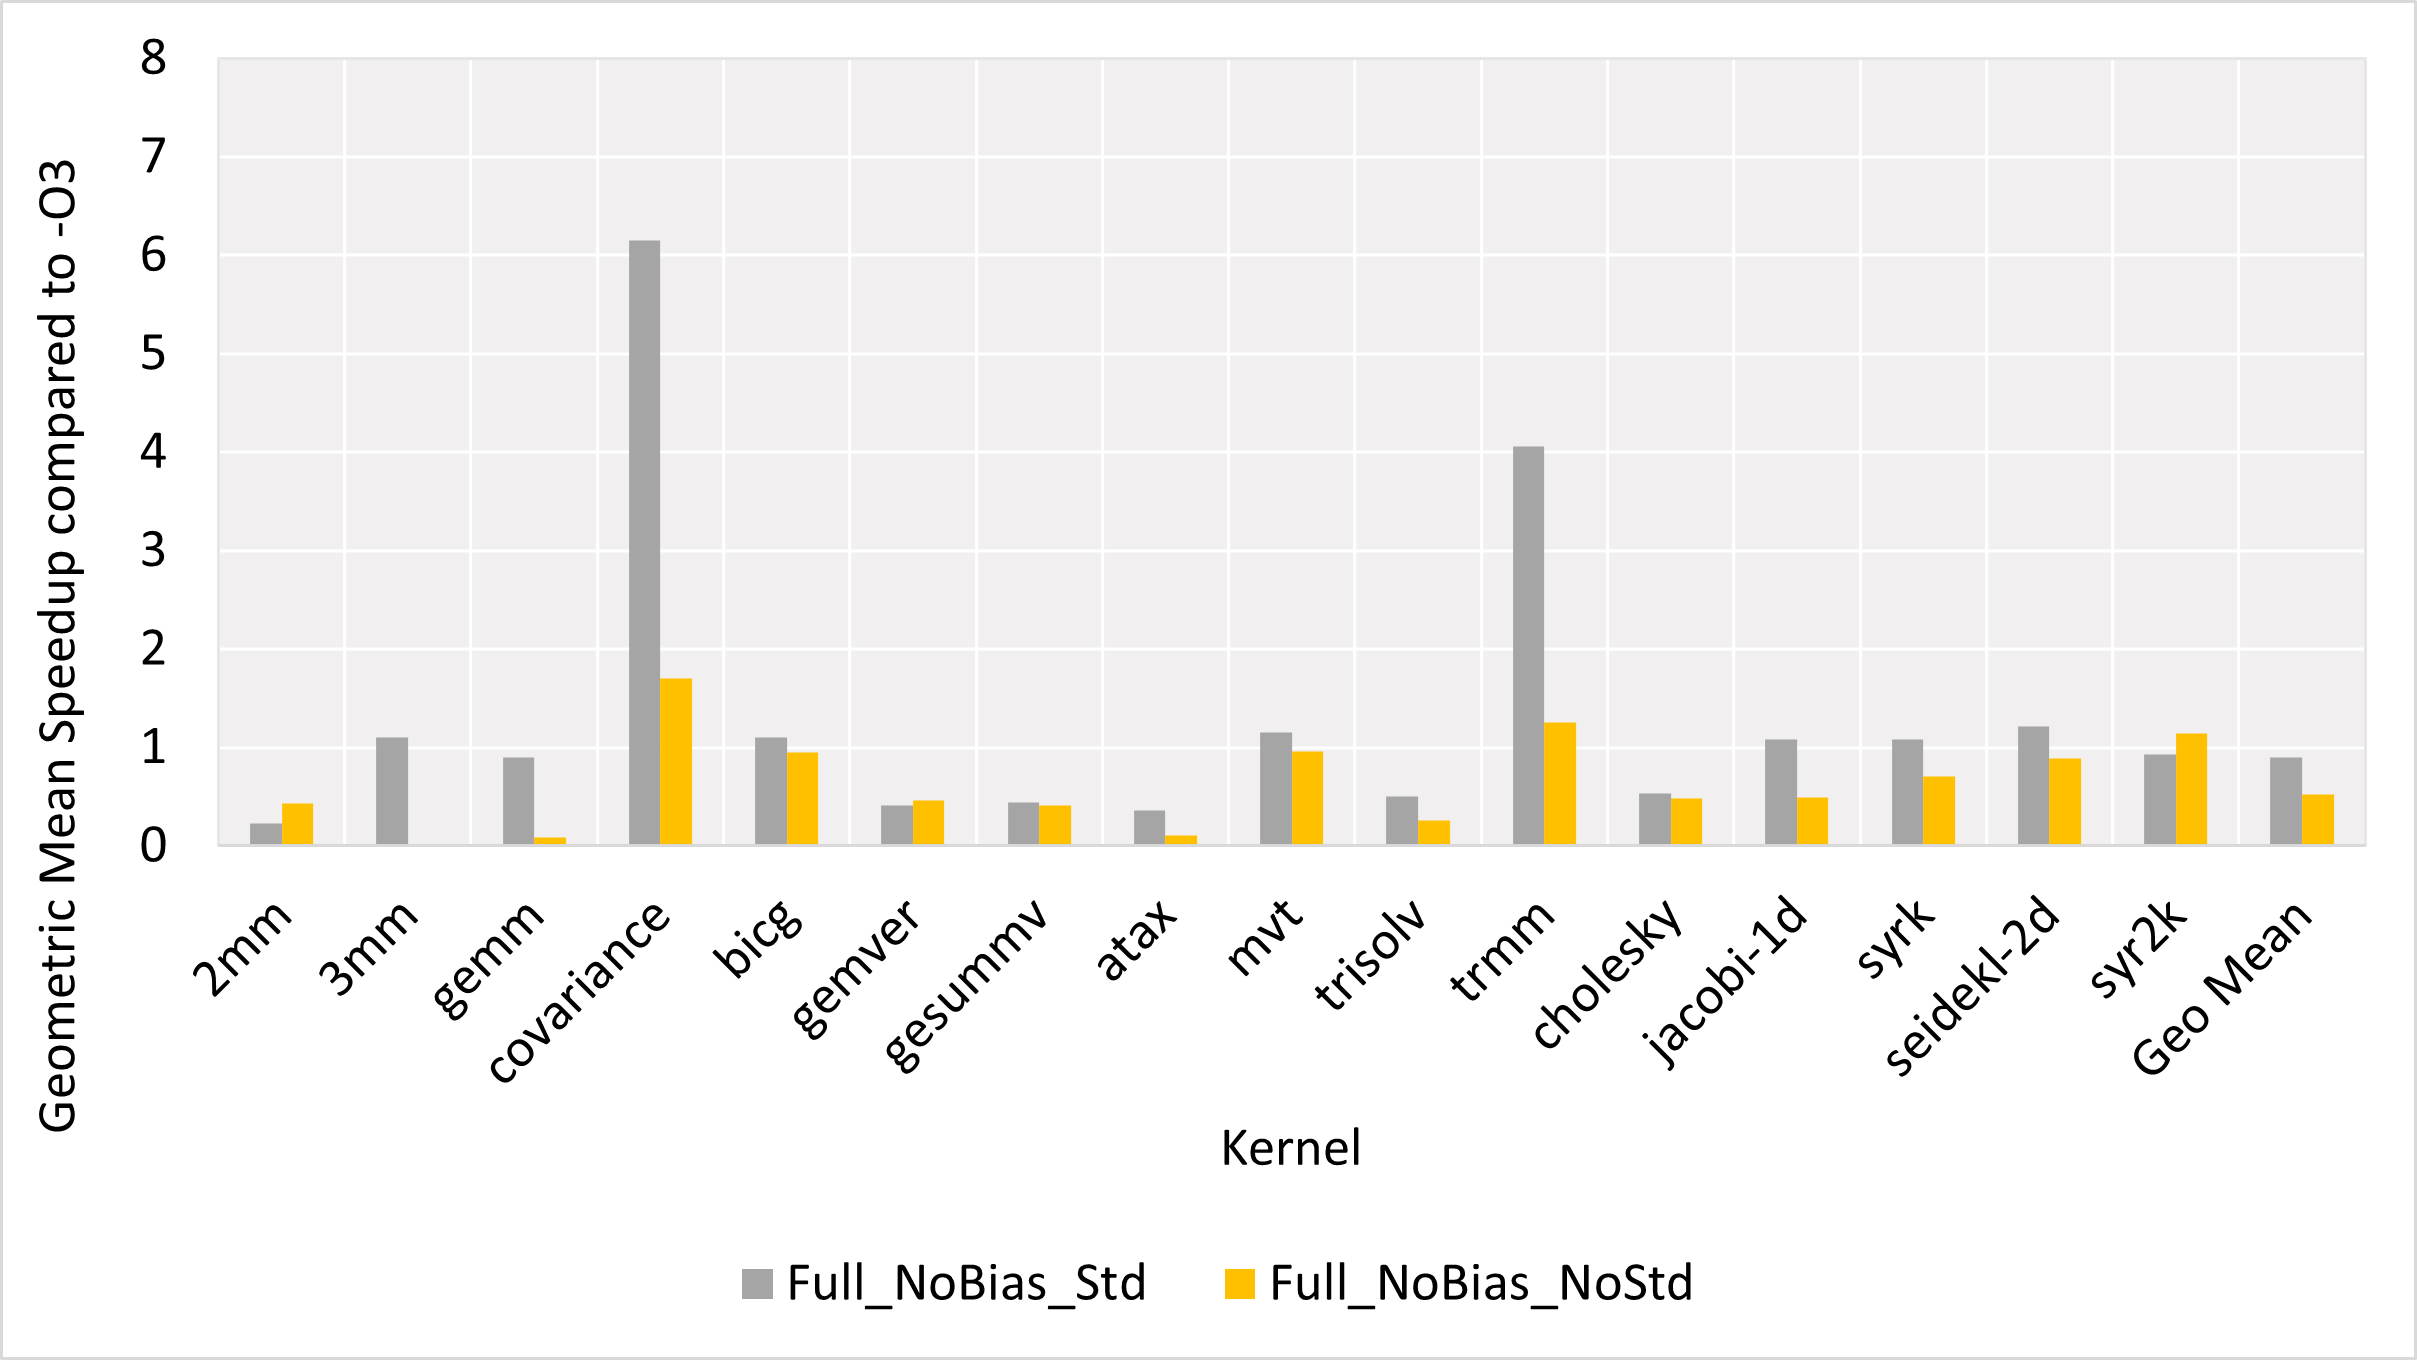
\includegraphics[width=0.8\textwidth]{Images/Compare_Std.png}   
  \caption{Analysis of standardisation approach}
  \label{fig:Compare_Std} 
\end{figure}

\begin{figure}[htbp]
  \centering
  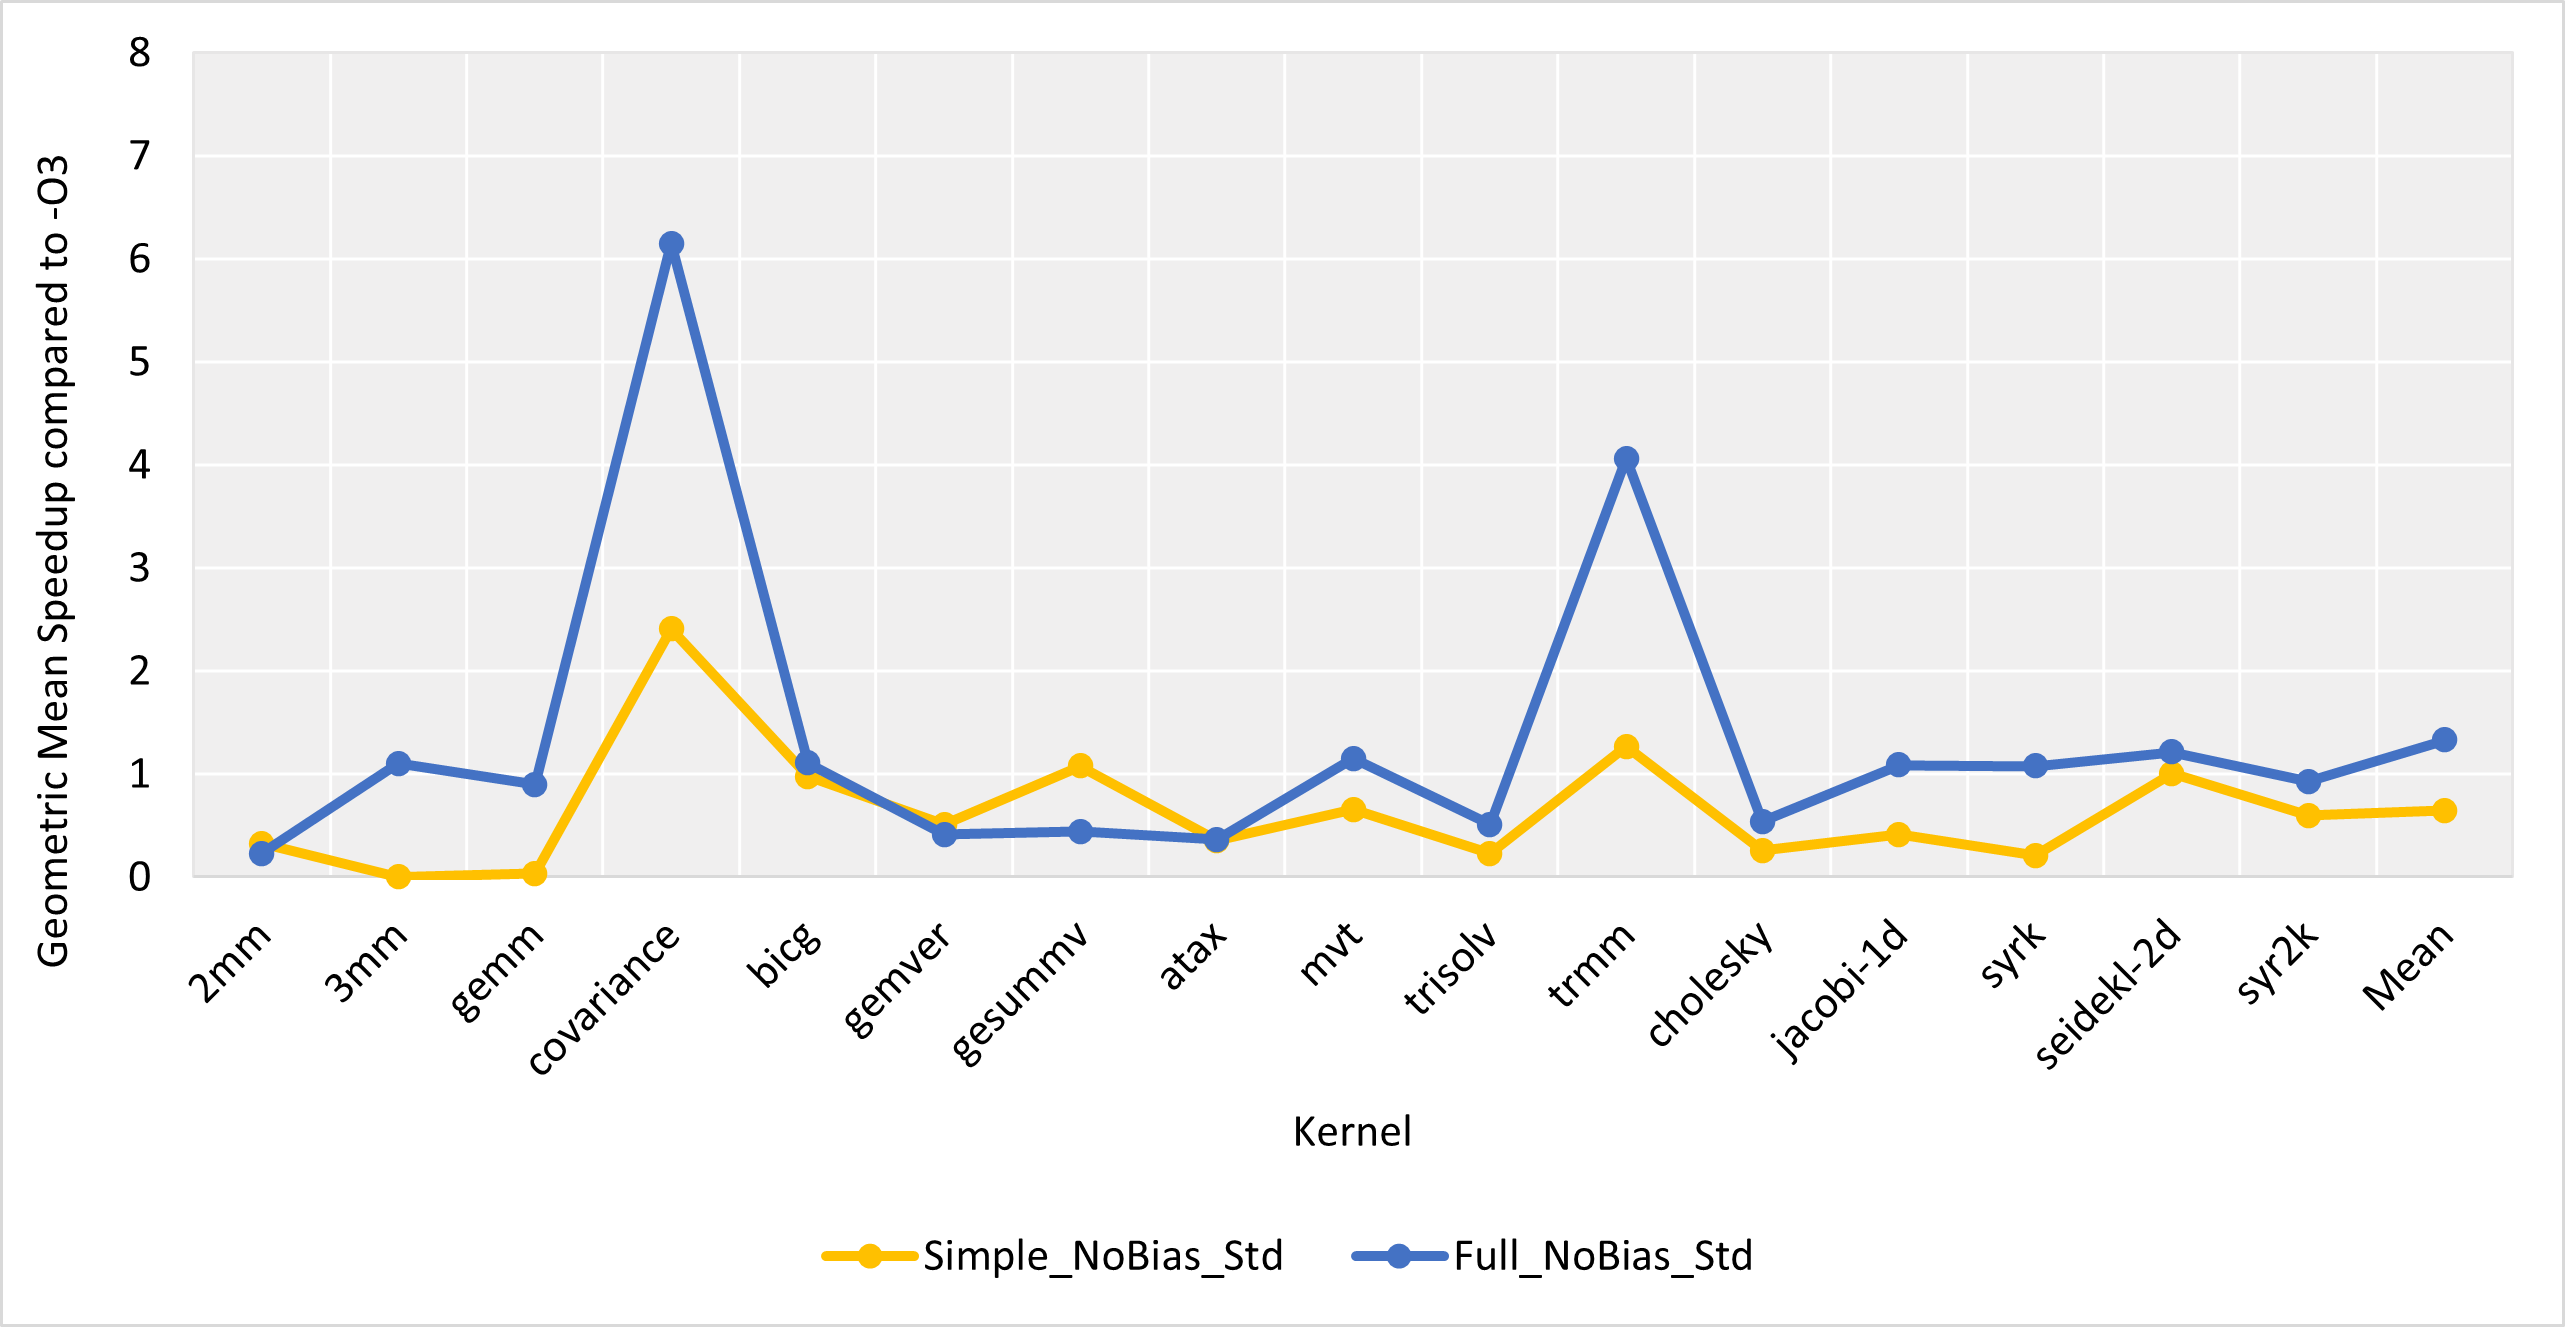
\includegraphics[width=0.8\textwidth]{Images/Compare_Rep.png}   
  \caption{Analysis of representation approach}
  \label{fig:Compare_Rep} 
\end{figure}

\begin{figure}[htbp]
  \centering
  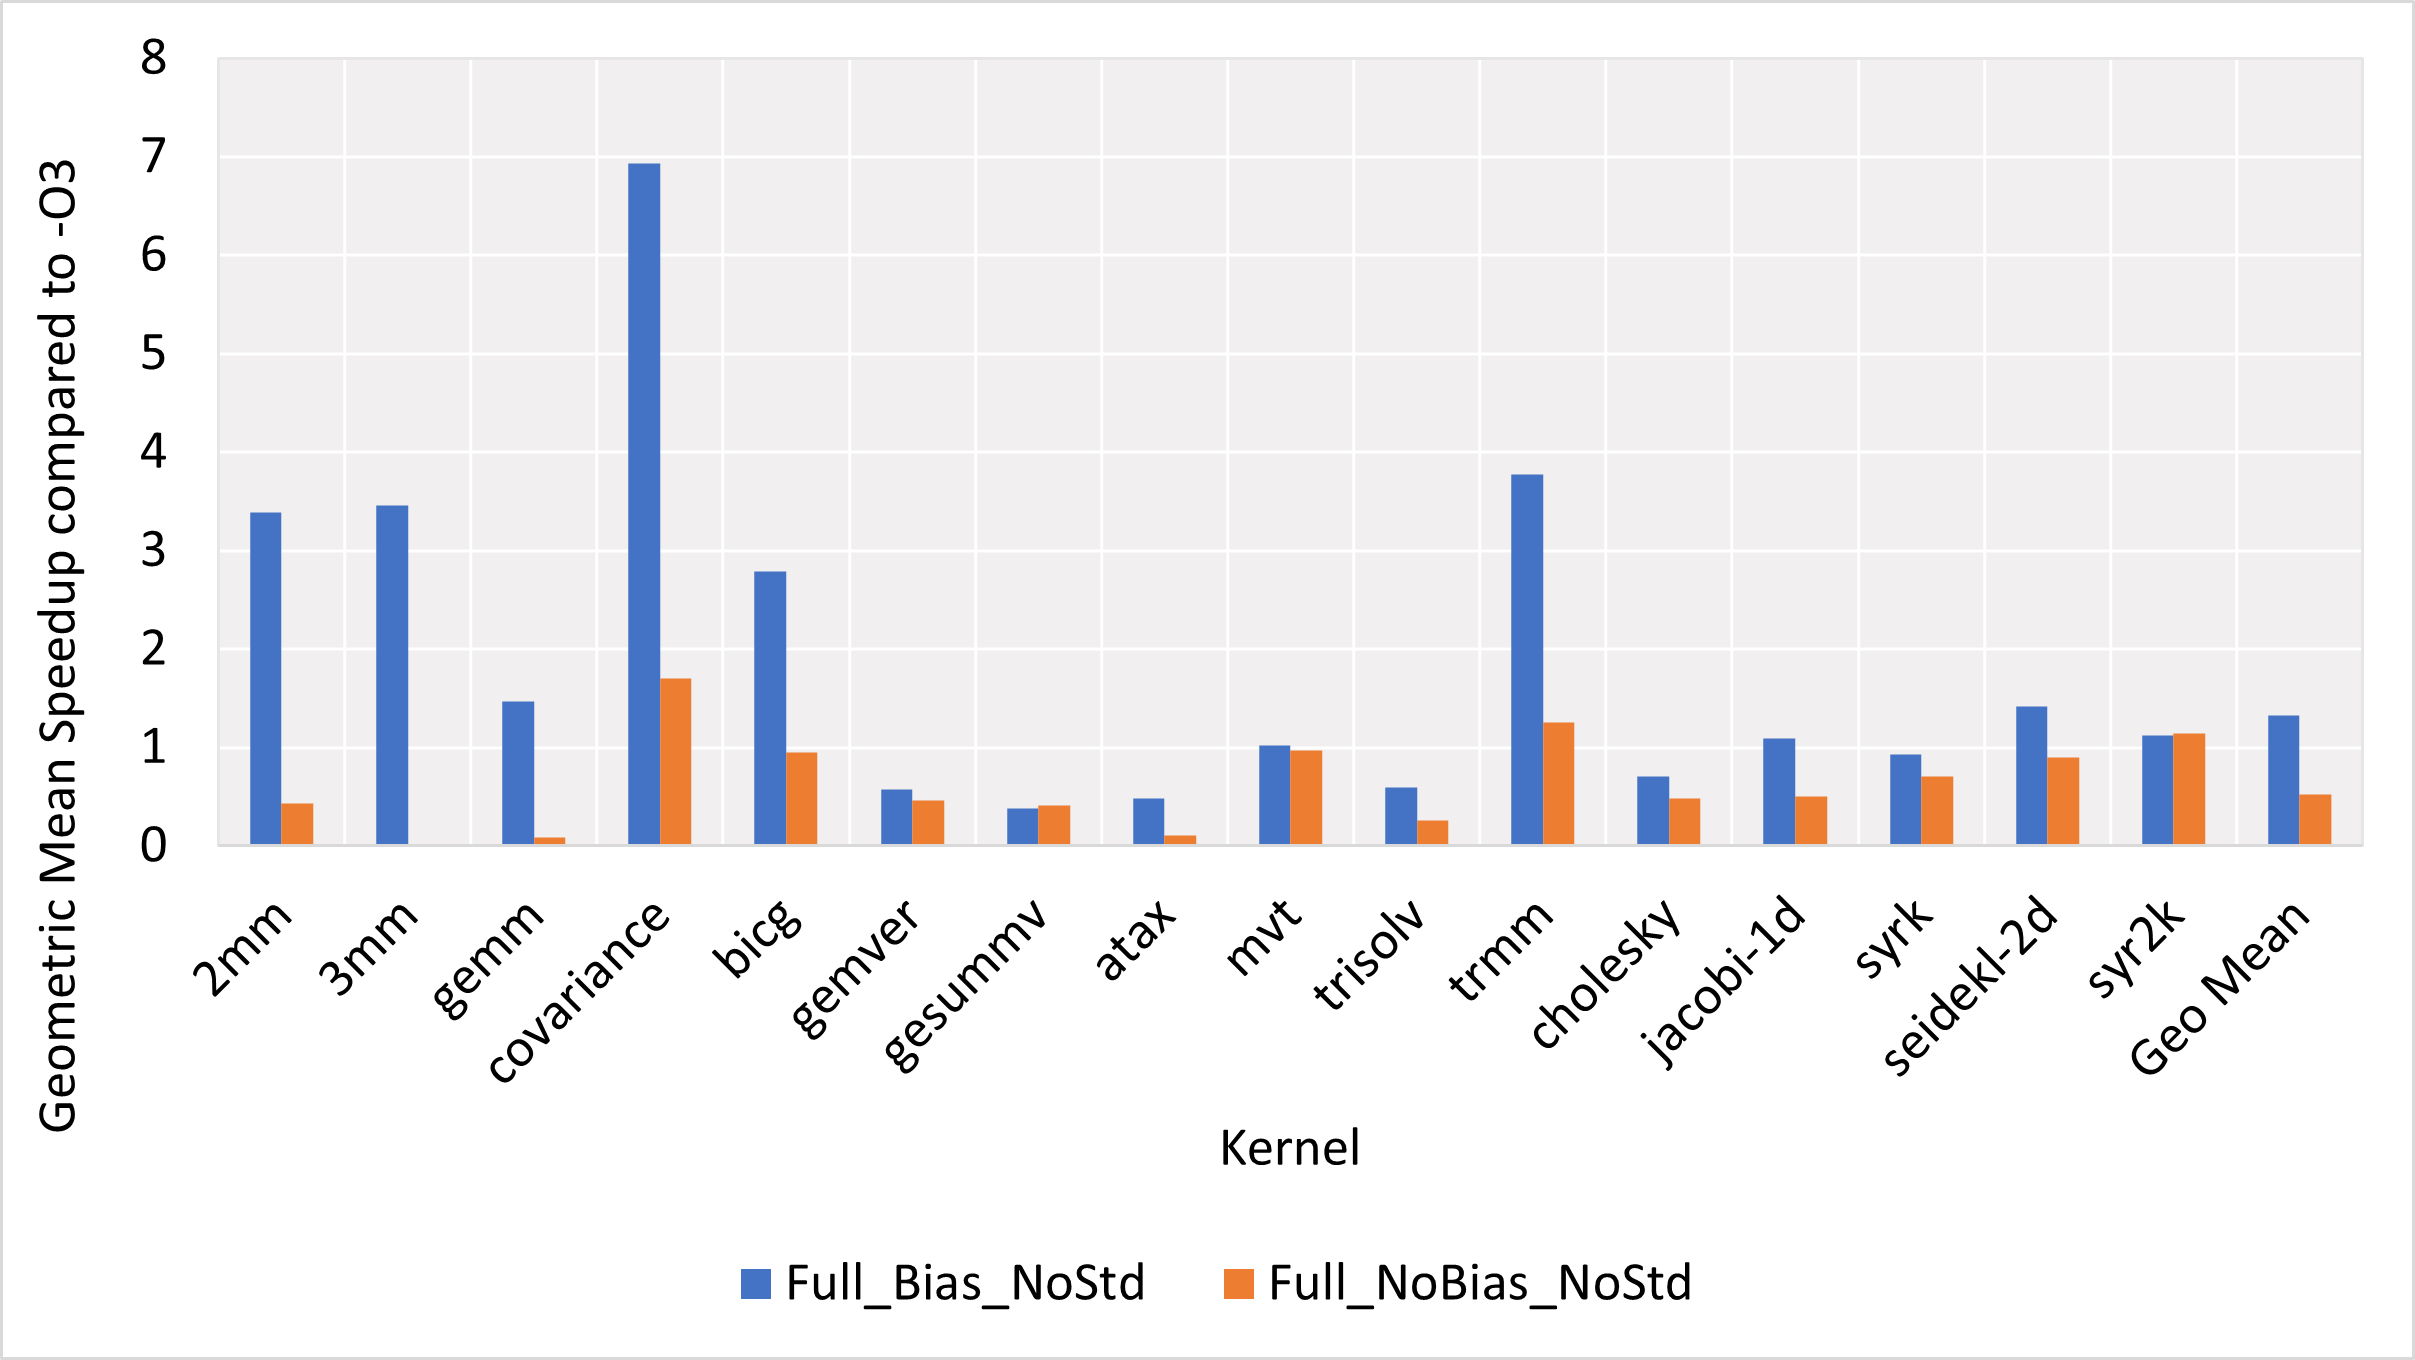
\includegraphics[width=0.8\textwidth]{Images/Compare_Bias.png}   
  \caption{Analysis of bias approach}
  \label{fig:Compare_Bias} 
\end{figure}

\chapter{Deep Learning Implementation}

\begin{algorithm}[H]
\caption{Update Agent Weights}\label{alg:weights_update}
\SetKwData{Left}{left}\SetKwData{This}{this}\SetKwData{Up}{up}
\SetKwFunction{Union}{Union}\SetKwFunction{FindCompress}{FindCompress}
\SetKwInOut{Input}{input}\SetKwInOut{Output}{output}
\Input{batch(transitions), reward, gamma}
\Output{q\_loss}

critics\_optim.zero\_grad()

predicted\_q \gets torch.gather(critics\_net(torch.tensor(batch.states)), 1, torch.tensor(batch.actions))

torch.no\_grad():

cal\_target \gets reward + gamma * (critics\_target(torch.tensor(batch.next\_states))) * (1-batch.done)
    
q\_loss \gets torch.mean(((cal\_target - predicted\_q.squeeze())**2))

q\_loss.backward()

critics\_optim.step()

update\_counter \gets = update\_counter + 1

 \If{update\_counter == target\_update\_freq}{
        critics\_target.hard\_update(critics\_net)
        
        update\_counter \gets 0$
    }
    
return q\_loss
\end{algorithm}

\end{document}

